\documentclass{article}

% Cabecera del documento
% ======================================================================

% Paquetes extras
\usepackage{matlab-prettifier}
\usepackage{ragged2e} % for \justifying
\usepackage[square, numbers, sort]{natbib}
% \usepackage{cite}
\usepackage{graphicx}
\usepackage[utf8]{inputenc}
\usepackage[T1]{fontenc}
\usepackage{amsmath,amssymb,amsfonts}
\usepackage{algorithmic}
\usepackage{textcomp}
\usepackage{subfig}
\usepackage{float}
\usepackage{mathtools}
\usepackage[spanish]{babel}
\usepackage[paper=a4paper,margin=2.75cm]{geometry}
\usepackage{booktabs} % for tables
\usepackage[colorlinks = true,
            linkcolor = blue,
            urlcolor  = blue,
            citecolor = orange,
            anchorcolor = blue]{hyperref} % for hyperlinks
\usepackage{makecell}
\usepackage{tikz}
\usetikzlibrary{positioning,arrows.meta}
\usepackage{appendix}
\usepackage{fancyhdr}
\usepackage{gensymb}
\usepackage{minted}
\usepackage{listings}
\usepackage[table]{xcolor}
% Soporte de caracteres acentuados del español dentro de lstlisting
\lstset{
  literate=
    {á}{{\'{a}}}1 {é}{{\'{e}}}1 {í}{{\'{i}}}1 {ó}{{\'{o}}}1 {ú}{{\'{u}}}1
    {Á}{{\'{A}}}1 {É}{{\'{E}}}1 {Í}{{\'{I}}}1 {Ó}{{\'{O}}}1 {Ú}{{\'{U}}}1
    {ñ}{{\~{n}}}1 {Ñ}{{\~{N}}}1
    {ü}{{\”u}}1 {Ü}{{\”U}}1
    {¿}{{?`}}1 {¡}{{!`}}1
}

\setlength{\headheight}{26pt} % ajusta si sale el warning “\headheight too small”
\definecolor{L-BLUE-1}{HTML}{5082CF}  

% tamaño de fuente para el header
\newcommand{\headerfont}{\fontsize{7pt}{8.5pt}\selectfont}


\fancypagestyle{fancyheader}{%
  \fancyhf{}            % limpia todo cabecera y pie

  % ---------- Encabezado ----------
  \fancyhead[C]{%
    \headerfont
    \makebox[\textwidth][c]{%
      % ----- minipage izquierda -----
      \begin{minipage}[b]{0.30\textwidth}
        \raggedright
        UNCUYO ---Ing.\ Mecatrónica\\
        Mendoza - Argentina
      \end{minipage}
      \hfill
      % ----- minipage central -----
      \begin{minipage}[b]{0.40\textwidth}
        \centering
        441 - PROYECTO FINAL DE ESTUDIOS\\
        Año 2026
      \end{minipage}
      \hfill
      % ----- minipage derecha -----
      \begin{minipage}[b]{0.25\textwidth}
        \raggedleft
        Martín Duci, Ignacio\\
        Legajo: 13560
      \end{minipage}
    }%
  }

  % línea horizontal bajo el encabezado
  \renewcommand{\headrulewidth}{0.8pt}

  % ---------- Pie ----------
  \fancyfoot[R]{\scriptsize \thepage}   % número pequeño, esquina derecha
  \renewcommand{\footrulewidth}{0pt}    % sin línea en el pie
}


% Directorio con imagenes
\graphicspath{{src/}}

% Titulo
\title{Diseño y simulación de un robot manipulador serial de seis grados de libertad para automatización logística.}

% Autores
\author{Ignacio Martín Duci \\ ignacio8martin@gmail.com \\ \\ Proyecto Final de Estudios (00441),\\ Facultad de Ingeniería, \\ Universidad Nacional de Cuyo, \\ \,\\Mendoza, Argentina \\ \\ Director: Ing. Eric Sánchez}

% Fecha
\date{Junio 2026}


% Cuerpo del documento
% ======================================================================
\begin{document}
\thispagestyle{empty}
\pagestyle{fancyheader}
\justifying

\maketitle
% ======================================================================
\newpage
\section*{Resumen}

Se presenta el diseño y la simulación de un robot manipulador serial de seis grados de libertad orientado a la automatización de procesos logísticos, específicamente a la transferencia de objetos entre contenedores (\textit{bin-to-bin transfer}). La motivación surge del crecimiento sostenido del mercado de robótica para depósitos, con tasas de expansión proyectadas entre el 17\,\% y el 22\,\% anual para Latinoamérica, región que presenta las mayores oportunidades relativas de automatización.

El desarrollo cubre el ciclo completo desde el modelado hasta la integración en software de robótica: se formula la cinemática directa mediante la convención Denavit-Hartenberg, se obtiene una solución analítica cerrada de la cinemática inversa con hasta 512 configuraciones articulares válidas, y se caracteriza el espacio de trabajo y las singularidades geométricas del manipulador (hombro, codo y muñeca). Sobre esta base se implementa un módulo de generación de trayectorias con interpolación en espacio articular y cartesiano, y escalado automático de velocidades y aceleraciones para respetar los límites cinemáticos. Los modelos CAD de cada eslabón se diseñaron en \textit{Fusion 360} y se integraron como mallas STL al entorno de simulación en MATLAB con la \textit{Robotics Toolbox} de Peter Corke. Finalmente, la cinemática y la generación de trayectorias se portaron a \textit{Robot Operating System 2} (ROS~2), construyendo una arquitectura de nodos con interfaces personalizadas, modelo URDF, visualización en RViz2 e interfaz gráfica de usuario desarrollada en PyQt5.

La simulación de la tarea completa de \textit{bin-to-bin transfer} confirma el cumplimiento de los límites cinemáticos impuestos y la coherencia entre los modelos MATLAB y ROS~2.

\medskip
\noindent\textbf{Palabras clave:} robot manipulador serial, seis grados de libertad, Denavit-Hartenberg, cinemática inversa analítica, planificación de trayectorias, Jacobiano geométrico, singularidades, MATLAB, Robotics Toolbox, Peter Corke, Fusion~360, ROS~2, URDF, RViz2, PyQt5, automatización logística, simulación robótica.

% ======================================================================
\newpage
\section*{Agradecimientos}

A la Facultad de Ingeniería de la Universidad Nacional de Cuyo, por los espacios de estudio y formación brindados. A sus docentes, por transmitir no solo conocimientos técnicos, sino también la pasión por la ingeniería.

\bigskip

A mi director, el Ing. Eric Sánchez, por acompañarme a lo largo de todo este proyecto con dedicación y generosidad. Por guiarme cuando el camino no era claro, por motivarme en los momentos difíciles, por confiar en el proyecto incluso antes de que tomara forma, y por el tiempo que destinó con genuino interés.

\bigskip

A mi familia y amigos, por estar presentes en cada etapa de esta carrera y en mi vida. Por el sostén incondicional, por celebrar cada logro como propio y por las horas compartidas dentro y fuera de la facultad. Su compañía fue, y es, indispensable.

\bigskip

A Dios.

% ======================================================================
\newpage
% INDICE
\tableofcontents

% ======================================================================
\newpage
\section{Introducción}

\subsection{Motivación y mercado}
La automatización e informatización de procesos de servicios es una trayectoria que, con el pasar de los años, aumenta su presencia en los diferentes mercados, brindando un aumento de la eficiencia, precisión, seguridad, operatividad y trazabilidad. Estos beneficios que brinda la implementación de tecnologías también quitan competitividad a aquellas entidades que, por disponibilidad, costo o falta de personal capacitado, no pueden implementar. 

Al revisar datos aportados por la consultora \href{https://www.grandviewresearch.com}{\textit{Grand View Research}},
 para analizar las proyecciones de mercado 2023-2030 para la robótica aplicada a depósitos logísticos o su traducción al ingles \textit{warehouses} para el mundo \cite{gvrGlobal2024}, Estados Unidos \cite{gvrUS2024}, China \cite{gvrChina2024}, Latinoamérica \cite{gvrLatAm2024} y Brasil \cite{gvrBrazil2024} pueden elaborarse las siguientes conclusiones.

\begin{enumerate}
    \item Todos los mercados proyectan un crecimiento anual compuesto de entre 17\% y 22.1\% lo cual se considera por encima de un escenario favorable.
    \item Comparativamente, Latinoamérica proyecta un escenario de crecimiento mayor al de Estados Unidos, China y al mundo en totalidad.
    \item Al analizar un país limítrofe que reporte datos como Brasil, puede verse que proyecta un crecimiento similar al de China en el período de tiempo analizado.
\end{enumerate}

Bajo estas conclusiones, puede entenderse que el mercado continuará creciendo, y que países con menores niveles de automatización e informatización serán los que presentarán mejores oportunidades para este campo. Si se considera la situación actual de Argentina, orientada a un modelo productivo con menor carga impositiva, puede posicionarse como plataforma estratégica para fabricar y exportar robótica de servicio.

En el contexto de la automatización de los procesos logísticos, la implementación de robots manipuladores es esencial para lograr movimientos en el espacio con alto grado de flexibilidad que permitan la reorganización de paquetes con alta precisión y eficiencia.

El desarrollo desde cero de un robot tipo serie de seis grados de libertad presenta una excelente oportunidad para integrar los conocimientos adquiridos en la carrera. También se presentarán desafíos que requerirán expandir conocimientos y aplicar nuevos conceptos y técnicas con criterio. La robótica serie es un campo profundamente estudiado, por lo que podrá accederse a una gran cantidad de información ya existente.

\subsection{Propuesta}
\label{sec:propuesta}

En el presente trabajo se desarrolla el diseño y la simulación de un robot manipulador serial de seis grados de libertad orientado a una aplicación específica: la transferencia de objetos entre contenedores (\textit{bin-to-bin transfer}).

Esta aplicación se plantea como un caso representativo dentro de procesos de manipulación en depósitos logísticos automatizados (\textit{micro-fulfillment warehouses}), permitiendo validar el desempeño del sistema en tareas típicas de pick-and-place.

La selección del caso de estudio se inspira en desarrollos industriales existentes, como el presentado en \href{https://www.youtube.com/watch?v=U2AGLeJBFNg\&t=172s}{YouTube}. No obstante, la solución propuesta en este trabajo es de desarrollo propio, enfocada en el modelado cinemático, la generación de trayectorias y la simulación del comportamiento del manipulador.

En la figura \ref{fig:aplicacion-vista-superior} puede verse un esquema de la aplicación descrita. 

\begin{figure}[H]
    \centering
    \includegraphics[width=0.85\linewidth]{vista_superior.png}
    \caption{Esquema de la aplicación - vista superior.}
    \label{fig:aplicacion-vista-superior}
\end{figure}

Mínimamente, se propone que el robot tenga un alcance de 500 mm, similar a las características del robot comercial \href{https://www.universal-robots.com/products/ur3e?utm_source=chatgpt.com}{UR3e}. En la figura \ref{fig:robot} se puede ver un esquema general de la morfología del robot.

\begin{figure}[H]
    \centering
    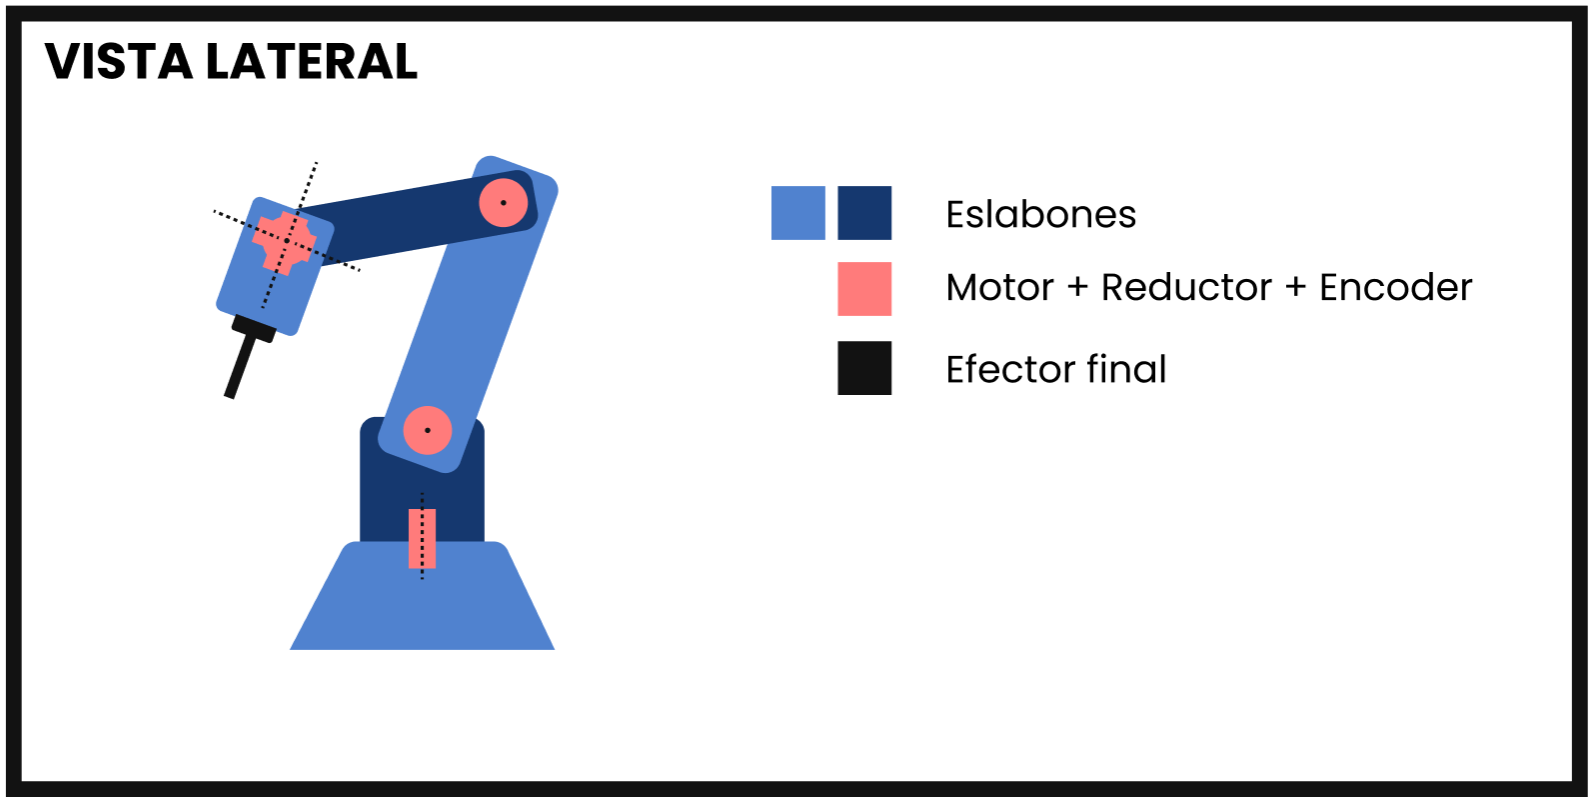
\includegraphics[width=0.85\linewidth]{robot.png}
    \caption{Esquema del robot tipo serie de 6 GDL propuesto.}
    \label{fig:robot}
\end{figure}


La tarea del robot consiste cronológicamente en lo siguiente:

\begin{enumerate}
    \item Roto-traslación a postura de espera de forma rápida.
    \item Roto-traslación a postura sobre caja origen a alta velocidad.
    \item Roto-traslación para \textit{picking} a baja velocidad.
    \item Roto-traslación hacia postura sobre caja origen a baja velocidad.
    \item Roto-traslación hacia postura sobre caja destino a alta velocidad.
    \item Roto-traslación para \textit{placing} a baja velocidad.
    \item Roto-traslación hacia postura sobre caja destino a baja velocidad.
    \item Repetir.
\end{enumerate}










% ======================================================================
\newpage
% INTRODUCCIÓN
\section{Objetivos y beneficiarios}
\label{sec:objetivos}

\,\\
\textbf{Objetivo mínimo:} Diseñar y simular un robot manipulador de seis ejes tipo serie con 500 mm de alcance destinado a tareas de \textit{bin-to-bin transfer} capaz de mover 300 elementos por hora.

Los siguientes objetivos se desarrollan en dos etapas: los ítems 1 a 6 corresponden a la implementación y validación en entorno MATLAB, mientras que los ítems subsiguientes se desarrollan en el entorno ROS 2.

\begin{enumerate}

    \item Definir las especificaciones del robot y su tarea.
    \item Realizar un diseño conceptual preliminar.
    \item Analizar y validar el espacio de trabajo. 
    \item Resolver analíticamente y validar la cinemática inversa.
    \item Implementar y validar un programa de generación de trayectorias que incorpore distintas funcionalidades, permitiendo la selección de modos de interpolación (cartesiana y articular) y la gestión de singularidades.
    \item Implementar, simular y validar la ejecución de la tarea definida, asegurando su correcto desempeño y cumplimiento de los objetivos planteados.
    \item Desarrollar un modelo CAD para simulaciones cinemáticas, asegurando la correspondencia entre los sistemas de referencia de cada componente y los marcos definidos mediante la convención Denavit–Hartenberg, a fin de garantizar consistencia geométrica y fidelidad en la representación del sistema en entornos de simulación.
    \item Desarrollar el modelo del robot en formato URDF a partir de la parametrización cinemática definida (DH), asegurando la correcta correspondencia entre eslabones y articulaciones.
    \item Integrar y verificar la coherencia de las geometrías CAD como representaciones visuales del modelo.
    \item Implementar el desarrollo de cinemática inversa, cinemática directa y generación de trayectorias en ROS 2.
    \item Desarrollar nodos de \textit{teaching} y gestión de trayectorias en ROS 2.
    \item Desarrollar nodo de interfaz de usuario gráfica que permita el movimiento manual, enseñanza y gestión de trayectorias del robot, así como análisis de variables cinemáticas en ROS 2.
    \item Implementar formato de descripción universal del robot (URDF) para simular con mayor estética el robot en entorno RViz.
\end{enumerate}


\medskip
\textbf{Posibles beneficiarios: }
\begin{enumerate}
    \item \textbf{Bodegas y agro-industria mendocina} que requieren automatizar el empaque y la manipulación de insumos sin invertir en robots industriales de alto costo.
    \item \textbf{Centros de \textit{micro-fulfillment} y PYMES logísticas} donde el brazo puede aumentar el \textit{pick-rate} y reducir tiempos de entrega.
    \item \textbf{Institutos y universidades locales} (UNCuyo, ITU, UTN) que obtendrán una plataforma didáctica \textit{open-source} para prácticas de mecatrónica y control.   
\end{enumerate}


% ======================================================================
\newpage
\section{Descripción de la tarea y especificaciones del robot}
\label{sec:tarea_especificaciones_robot}

La tarea del manipulador consiste en la transferencia de objetos entre dos contenedores de dimensiones y posiciones predefinidas. Esto puede verse en las figuras \ref{fig:tarea_superior} y \ref{fig:tarea_lateral} donde también quedan definidos puntos clave de la trayectoria que deberá seguir el robot conforme a lo definido en la sección \ref{sec:propuesta}.

\begin{figure}[H]
    \centering
    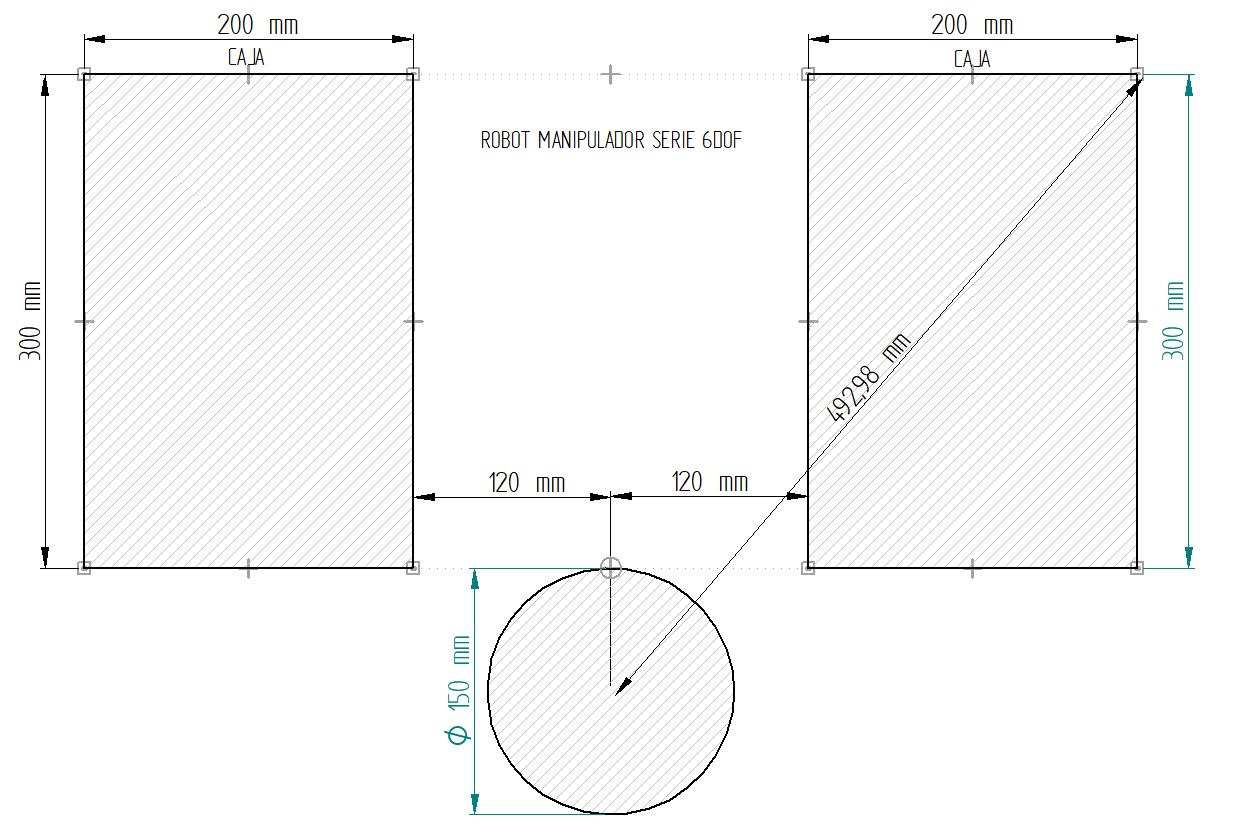
\includegraphics[width=0.85\linewidth]{VISTA_SUPERIOR.png}
    \caption{Vista superior del robot y la tarea}
    \label{fig:tarea_superior}
\end{figure}

\begin{figure}[H]
    \centering
    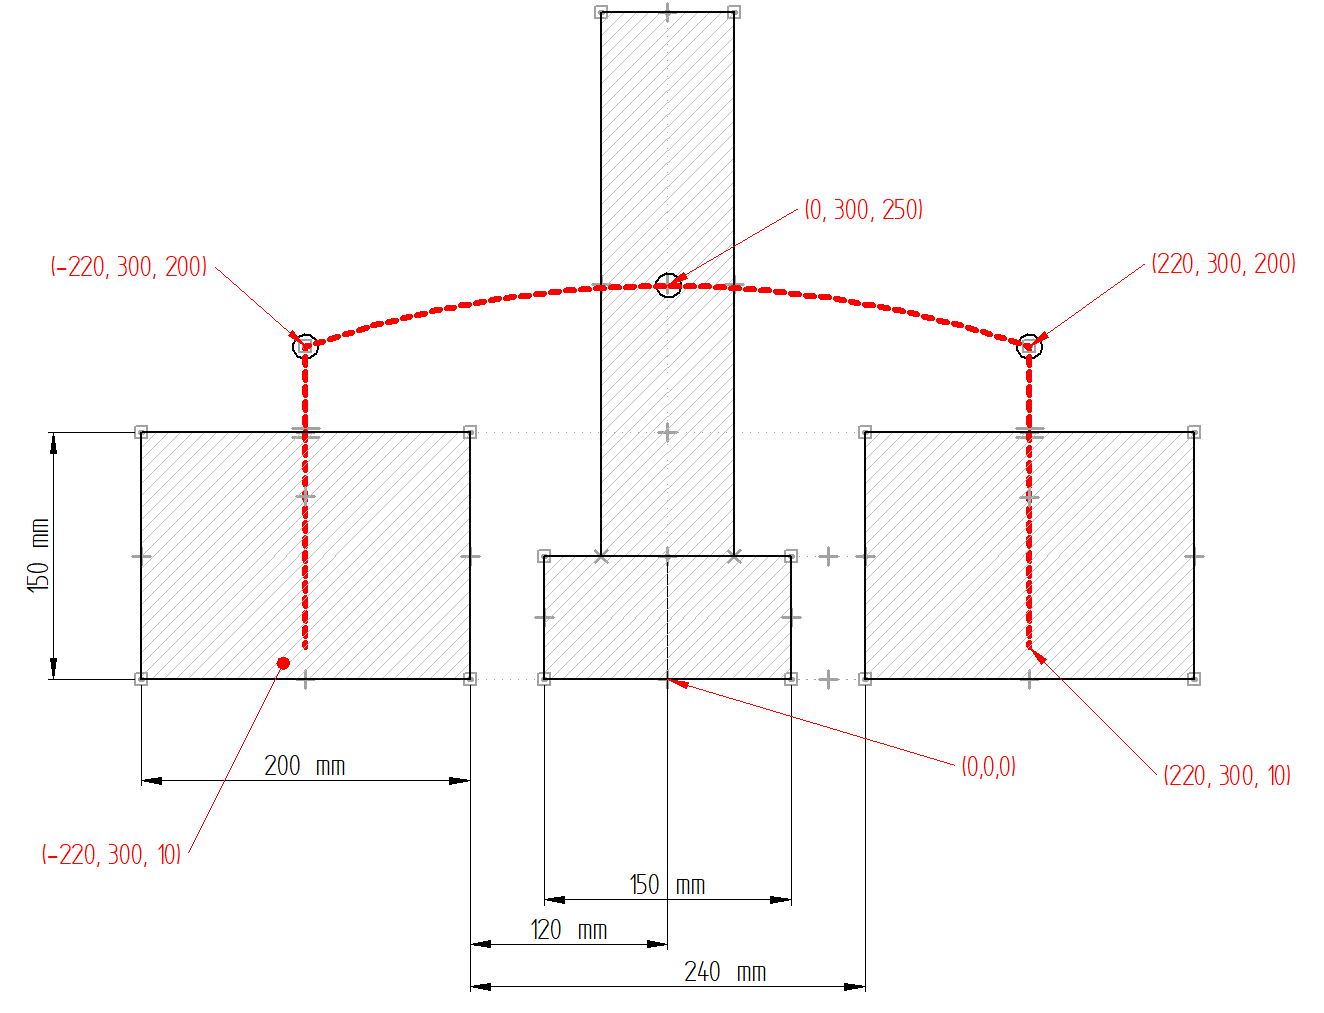
\includegraphics[width=0.85\linewidth]{VISTA_LATERAL.png}
    \caption{Vista lateral del robot y la tarea}
    \label{fig:tarea_lateral}
\end{figure}

Los objetos serán tomados mediante un sistema de sujeción por vacío (ventosa - \textit{vacuum gripper}) y depositados mediante la liberación del mismo, esto permite relajar los requerimientos de precisión y repetibilidad del manipulador.

\subsection*{Especificaciones del proyecto}

Quedan definidas las especificaciones del manipulador que son objeto del presente trabajo:

\begin{itemize}
    \item Grados de libertad (GDL - \textit{DOF}): 6.
    \item Alcance: 500.00 mm
    \item Rango articulaciones 1 a 5: $\pm2\pi$
    \item Rango articulación final: \textit{libre}
\end{itemize}

\subsection*{Especificaciones para posible extensión del proyecto}

Las siguientes especificaciones quedan definidas como referencia para desarrollos posteriores que aborden el diseño mecánico, el control de fuerza y la integración con el entorno físico:

\begin{itemize}
    \item Capacidad de carga útil: 3.00 kg
    \item Precisión: 0.5 mm
    \item Repetibilidad: 0.5 mm
    \item Temperatura ambiente entre 5 y 35 ºC.
    \item Humedad relativa $\leq 70\%$.
    \item Bajo nivel de polvo ambiental.
    \item Iluminación 100-150 lx.
    \item Entorno sin vibraciones.
    \item Protección IP54
\end{itemize}


% ======================================================================
\newpage
\section{Diseño conceptual preliminar}
\label{sec:diseno_conceptual_preliminar}

Con el objetivo de tener un punto de partida en cuanto a la morfología y dimensiones del robot, tomando como referencia al robot \href{https://www.universal-robots.com/products/ur3e?utm_source=chatgpt.com}{UR3e}, se define la siguiente estructura, morfología y dimensiones:

\begin{figure}[H]
    \centering
    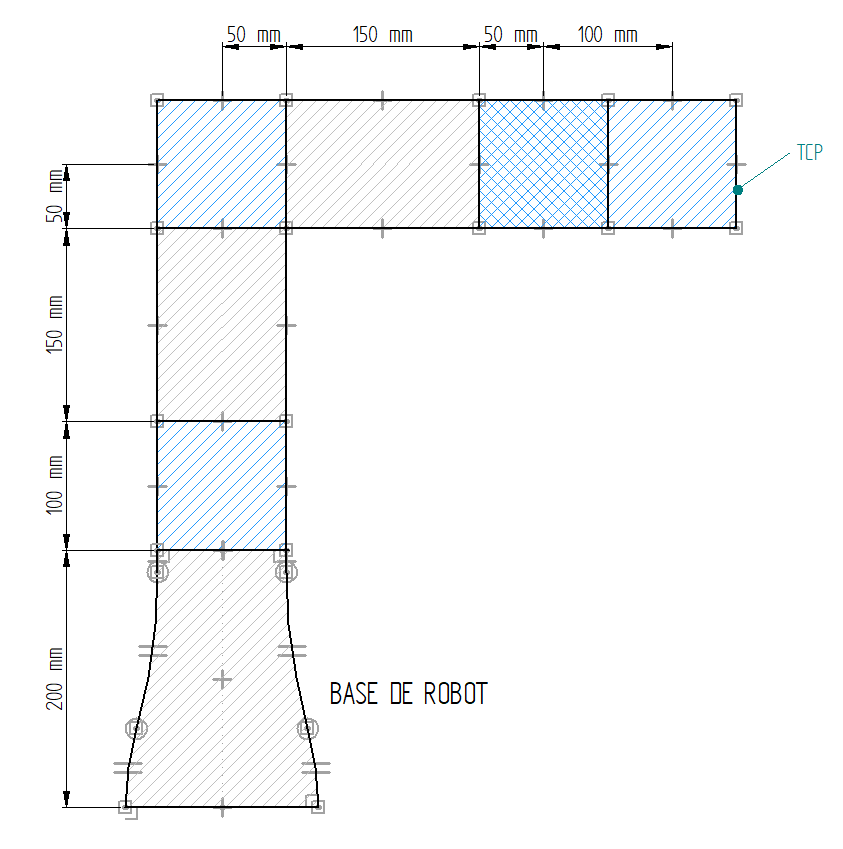
\includegraphics[width=0.75\linewidth]{DIM_ROBOT_1.png}
    \caption{Vista lateral 1 de un esquema del robot}
    \label{fig:dim_robot_1}
\end{figure}

\begin{figure}[H]
    \centering
    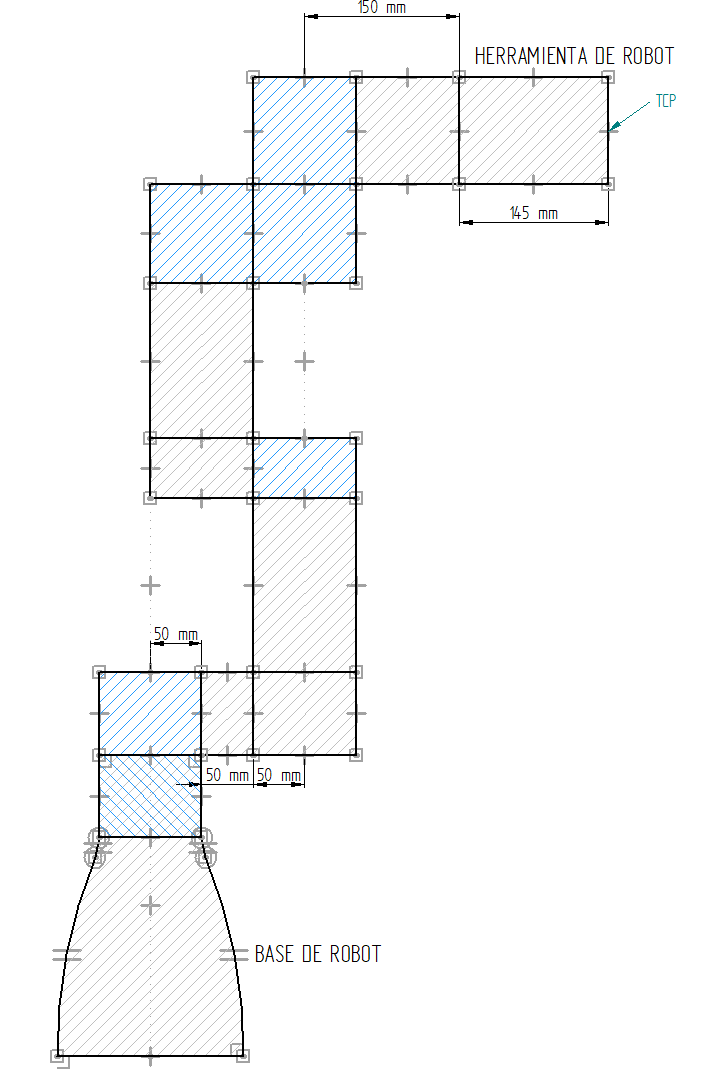
\includegraphics[width=0.75\linewidth]{DIM_ROBOT_2.png}
    \caption{Vista lateral 2 del un esquema del robot}
    \label{fig:dim_robot_2}
\end{figure}

A partir de estas imágenes se obtiene la información necesaria para la elaboración del modelo cinemático. Se ha incorporado una base para permitir que el robot opere de forma segura por encima de las cajas y una herramienta final tipo ventosa (\textit{vacuum-gripper}), para esta última se toma como referencia el modelo \textit{EPick with one suction cup 145x83 mm} del fabricante \href{https://robotiq.com/es/productos/pinzas-vacuum}{\textit{Robotiq}}.





% ======================================================================
\newpage
\section{Modelado cinemático}
\label{sec:cinematica}

En esta sección se aborda el modelado cinemático del manipulador, así como la resolución de la cinemática inversa y la planificación de trayectorias necesarias para su operación.

El modelado cinemático permite establecer la relación entre las variables articulares del robot y la posición y orientación de su efector final. A partir de este modelo, se plantea la resolución de la cinemática inversa, con el objetivo de determinar las configuraciones articulares requeridas para alcanzar posiciones específicas dentro del espacio de trabajo.

Finalmente, se desarrolla la planificación de trayectorias, mediante la cual se define la evolución temporal del movimiento del manipulador entre distintas configuraciones, garantizando continuidad, suavidad y seguridad en su ejecución.

%
% ============
%
\subsection{Modelado cinemático}
\label{sec:modelado_cinematico}

Para obtener el modelo cinemático se aplica el algoritmo Denavit-Hartenberg estándar el cual consiste en lo siguiente:

\begin{enumerate}
    \item Enumerar los n+1 eslabones desde 0 hasta n, comenzando desde la base (eslabón fijo) y terminando en el efector final.
    \item Identificar los ejes de cada articulación. Si es rotacional, será el eje de giro; si es prismática, será el eje a lo largo del cual se produce el desplazamiento.
    \item Enumerar los ejes de 1 a n, comenzando desde el que une el eslabón base con el eslabón 1.
    \item Para i de 0 a n-1, situar el eje $Z_1$ en el eje de la articulación i+1.
    \item El eje $Z_n$ se colocará en el extremo del último eslabón en la misma dirección que el eje $Z_{n-1}$.
    \item Situar el origen del sistema de la base $\{S_0\}$ en cualquier punto del eje $Z_0$.
    \item Para $i = 1$ a $n$, ubicar el sistema $\{S_i\}$ en la intersección entre el eje $Z_i$ y la recta perpendicular común a los ejes $Z_i$ y $Z_{i-1}$. En caso de que los ejes $Z_i$ y $Z_{i-1}$ se intersecten, el sistema $\{S_i\}$ se posiciona en dicho punto de intersección.
    \item Para $i = 1$ a $n$, definir el eje $X_i$ a partir del punto donde se estableció el sistema $\{S_i\}$, sobre la recta perpendicular común a los ejes $Z_i$ y $Z_{i-1}$. Si los ejes $Z_i$ y $Z_{i-1}$ se intersectan, el eje $X_i$ debe ser perpendicular a ambos. Su orientación puede elegirse de forma arbitraria.
    \item El eje $X_0$ puede definirse libremente, siendo conveniente alinearlo con el eje $X_1$.
    \item Para $i = 0$ a $n$, definir el eje $Y_i$ de manera que, junto con los ejes $X_i$ y $Z_i$, forme un sistema de referencia dextrógiro.
    
\end{enumerate}

Luego se determinan los parámetros que permitirán elaborar una matriz que define al robot en cuestión de la siguiente forma:

Para $i = 1$ a $n$:

\begin{enumerate}
    \item $\theta_i$: Ángulo alrededor del eje $Z_{i-1}$, desde el eje $X_{i-1}$ hasta el eje $X_i$.
    
    \item $d_i$: Distancia a lo largo del eje $Z_{i-1}$, desde el origen del sistema $i-1$ hasta el eje $X_i$.
    
    \item $a_i$: Distancia a lo largo del eje $X_i$, desde el eje $Z_{i-1}$ hasta el eje $Z_i$.
    
    \item $\alpha_i$: Ángulo alrededor del eje $X_i$, desde el eje $Z_{i-1}$ hasta el eje $Z_i$.
\end{enumerate}

\medskip

Donde:

\begin{itemize}
    \item $a_i$: Longitud del eslabón.
    \item $\alpha_i$: Ángulo de torsión del eslabón.
    \item $d_i$: Longitud articular.
    \item $\theta_i$: Ángulo articular.
\end{itemize}

Utilizando esta información, los parámetros de Denavit-Hartenberg pueden organizarse en la siguiente forma general:

\begin{equation}
\begin{array}{c|cccc}
i & \theta_i & d_i & a_i & \alpha_i \\
\hline
1 & \theta_1 & d_1 & a_1 & \alpha_1 \\
2 & \theta_2 & d_2 & a_2 & \alpha_2 \\
\vdots & \vdots & \vdots & \vdots & \vdots \\
n & \theta_n & d_n & a_n & \alpha_n \\
\end{array}
\end{equation}

Finalmente, se ha conseguido describir la geometría del robot y la interrelación entre sus eslabones mediante un algoritmo. El beneficio de esta representación radica en que permite determinar la posición y orientación de cada sistema de referencia a partir del anterior y, por consiguiente, obtener la posición y orientación del efector final en función de las variables articulares. A continuación, se presenta de forma general la matriz de transformación homogénea que relaciona cada sistema de referencia con el anterior.

\begin{equation}
{}^{i-1}T_i =
\begin{bmatrix}
\cos\theta_i & -\sin\theta_i \cos\alpha_i & \sin\theta_i \sin\alpha_i & a_i \cos\theta_i \\
\sin\theta_i & \cos\theta_i \cos\alpha_i  & -\cos\theta_i \sin\alpha_i & a_i \sin\theta_i \\
0            & \sin\alpha_i               & \cos\alpha_i               & d_i \\
0            & 0                          & 0                          & 1
\end{bmatrix}
\end{equation}

Puede entonces determinarse, para un robot de 6 grados de libertad, la posición y orientación del efector final en función de las variables articulares mediante la transformación sucesiva del sistema base hasta el sistema herramienta.

\begin{equation}
    {}^{base}T_{tcp} = {}^{b}T_0 {}^{0}T_1 \,\,\,\,...\,\,\,\, {}^{5}T_6 {}^{6}T_tcp
\end{equation}

De esta forma quedará definida \textbf{el modelo cinemático directo}.

Se obtiene información sobre las dimensiones del robot de la figura \ref{fig:dim_robot_1} y \ref{fig:dim_robot_2} y se elabora el siguiente esquema simplificado con información solo esencial al aplicar el algoritmo DH:

\begin{figure}[H]
    \centering
    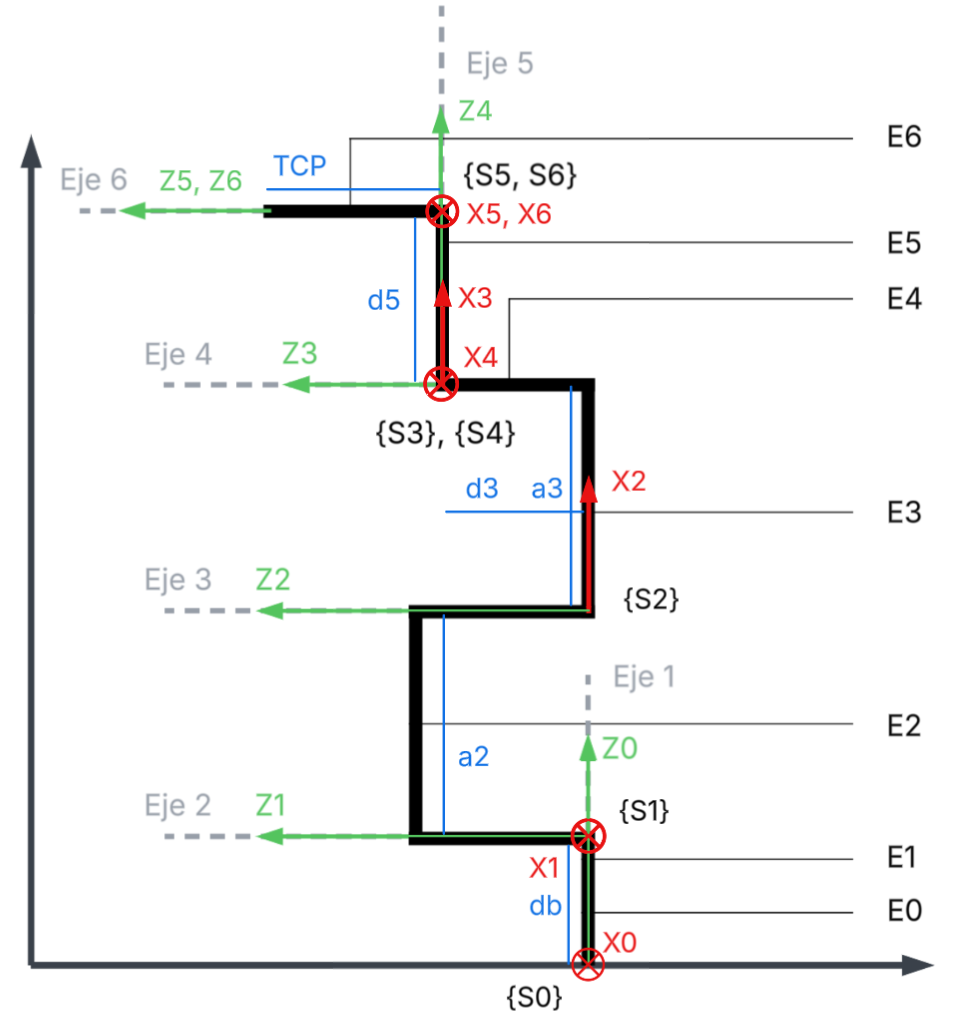
\includegraphics[width=0.55\linewidth]{DH.png}
    \caption{Algoritmo DH aplicado a un esquema simplificado del robot}
    \label{fig:DH}
\end{figure}

Teniendo en cuenta que las articulaciones son de tipo rotacional, la variable articular será $\theta$ para todos los casos. Se define la matriz Denavit-Hartenberg a partir de la información de la figura \ref{fig:DH} y del procedimiento definido en la explicación del algoritmo:

\begin{equation}
\begin{array}{c|llll}
i & \theta_i [rad] & d_i [m]& a_i [m]& \alpha_i [rad]\\
\hline
1 & q_1                 & 0.25     & 0     & \frac{-pi}{2}\\
2 & q_2-\frac{pi}{2}    & 0     & 0.25  & 0 \\
3 & q_3                 & 0.295  & 0.25  & 0 \\
4 & q_4+\frac{pi}{2}    & 0     & 0     & \frac{pi}{2} \\
5 & q_5                 & 0.1   & 0     & \frac{-pi}{2} \\
6 & q_6                 & 0     & 0     & 0 \\
\end{array}
\end{equation}

Notas:
\begin{itemize}
    \item Mediante la letra \textit{"q"} se simboliza el parámetro variable.
    \item La suma o resta a valores de \textit{q}, como lo es en los casos 2 y 4, dan un offset de posición que modifica el punto cero del robot.
\end{itemize}


%
% ============
%
\subsection{Análisis y verificación de espacio de trabajo }
\label{sec:espacio_trabajo}

Para verificar el alcance máximo y la tarea de nuestro robot, simplemente buscamos una posición de alto estiramiento ($q=[variable,\frac{pi}{2},0,-\frac{pi}{2},-\frac{pi}{2},0]$) y se ingresan valores progresivos completando el giro de la primera articulación. Luego, esto produce el siguiente resultado (script \colorbox{gray!20}{\texttt{test\_workspace.m}}):

\begin{figure}[H]
    \centering
    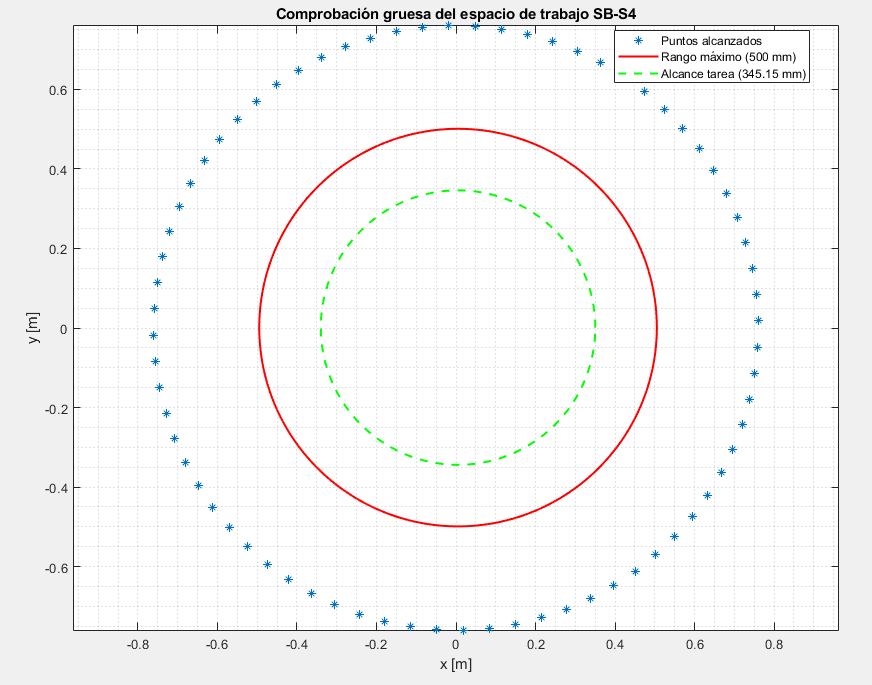
\includegraphics[width=0.85\linewidth]{test_workspace_1.png}
    \caption{Verificación de espacio de trabajo en plano XY}
    \label{fig:workspace_1}
\end{figure}

%
% ============
%
\subsection{Cinemática inversa}
\label{sec:cinemática_inversa}

En el desarrollo cinemático de todo robot es fundamental elaborar el modelo de cinemática inversa, el cual permite determinar las variables articulares necesarias para alcanzar una posición y orientación deseadas del efector final. En este trabajo, la resolución se aborda mediante un enfoque analítico, obteniendo expresiones en forma cerrada que relacionan directamente las variables del espacio cartesiano con las variables articulares, evitando el uso de métodos numéricos iterativos.

Se parte de la observación de que el manipulador no cuenta con una muñeca esférica; es decir, los tres ejes correspondientes a la muñeca no se intersectan en un mismo punto, lo que no nos permite hacer uso del método de Pieper.

En esta resolución, se implementan métodos algebraicos para separar incógnitas y determinarlas en función de parámetros conocidos y variables ya determinadas.

Dado que se ha definido el modelo cinemático directo al haber elaborado la matriz Denavit-Hartenberg se conocen todas las matrices de transformación homogénea, particularmente:
\begin{equation}
    T^{base}_{tcp}, T^{base}_0, T^6_{tcp}
\end{equation}
Al desacoplar la base y la herramienta final se puede conocer:

\begin{equation}
\label{eq:ci_desacople}
    T^0_6=[T^{base}_0]^{-1}T^{base}_{tcp}[T^6_{tcp}]^{-1}
\end{equation}

También se sabe que:

\begin{equation}
    T^0_6=T^0_1T^1_2T^2_3T^3_4T^4_5T^5_6
\end{equation}

En esta ecuación hay una alta complejidad en el lado derecho (RHS) y una baja complejidad en el lado izquierdo (LSH) por lo que se equilibra de la siguiente manera:

\begin{equation}
    \label{eq:ci_1}
    [T^0_1]^{-1}T^0_6[T^5_6]^{-1} = T^1_2T^2_3T^3_4T^4_5
\end{equation}

De forma genérica la matriz de transformación homogénea que vincula al sistema $i-1$ con el sistema $i$ es:

\begin{equation}
T^{i-1}_i =
\begin{bmatrix}
c_i & -s_i c_j & s_i s_j & a_i 
c_i \\
s_i & c_i c_j  & -s_i s_j & a_i
s_i \\
0            & s_j               & c_j               & d_i \\
0            & 0                          & 0                          & 1
\end{bmatrix}
\label{eq:ci_2}
\end{equation}

Donde:

\begin{equation}
\begin{aligned}
    s_i &:= \sin(\theta_i) \\
    c_i &:= \cos(\theta_i) \\
    s_j &:= \sin(\alpha_i) \\
    c_j &:= \cos(\alpha_i) 
\end{aligned}
\end{equation}

\textbf{NOTA:} El subíndice i y j no indican sistemas diferentes sino que i hace referencia al ángulo $\theta$ y j al ángulo $\alpha$ para simplificar la nomenclatura de las funciones.

Cada matriz de transformación homogénea esta compuesta por cuatro partes:

\[
\left[T_i^{\,i-1}\right]
=
\begin{bmatrix}
R_{3x3} & p_{3x1} \\
0\ 0\ 0 & 1
\end{bmatrix}
\]

Se puede obtener la matriz de transformación homogénea inversa mediante la siguiente expresión:

\[
\left[T_i^{\,i-1}\right]^{-1}
=
\begin{bmatrix}
R^T & -R^T T \\
0\ 0\ 0 & 1
\end{bmatrix}
\]

\[
R^T =
\begin{bmatrix}
c_i & s_i & 0 \\
- s_i c_j & c_i c_j & s_j \\
s_i s_j & -c_i s_j & c_j
\end{bmatrix}
\]

\[
p =
\begin{bmatrix}
a_i c_i \\
a_i s_i \\
d_i
\end{bmatrix}
\]

\[
- R^T p =
\begin{bmatrix}
- c_i & - s_i & 0 \\
+ s_i c_j & - c_i c_j & - s_j \\
- s_i s_j & + c_i s_j & - c_j
\end{bmatrix}
\begin{bmatrix}
a_i c_i \\
a_i s_i \\
d_i
\end{bmatrix}
=
\begin{bmatrix}
- a_i \\
- d_i s_j \\
- d_i c_j
\end{bmatrix}
\]

Y se obtiene la matriz de transformación homogénea inversa:

\[
\left[T_i^{\,i-1}\right]^{-1}
=
\begin{bmatrix}
c_i & s_i & 0 & -a_i \\
- s_i c_j & c_i c_j & s_j & -d_i s_j \\
s_i s_j & -c_i s_j & c_j & -d_i c_j \\
0 & 0 & 0 & 1
\end{bmatrix}
\]

Se toma esta plantilla de matriz y la plantilla de la matriz \ref{eq:ci_2}, se reemplazan valores y se simplifican para formar las matrices de transformación homogéneas presentes en la ecuación \ref{eq:ci_1}.

\[
\left[T_1^{\,0}\right]^{-1} =
\begin{bmatrix}
c_1 & s_1 & 0 & 0 \\
0 & 0 & -1 & d_1 \\
- s_1 & c_1 & 0 & 0 \\
0 & 0 & 0 & 1
\end{bmatrix}
\]

\[
\left[T_6^{\,5}\right]^{-1} =
\begin{bmatrix}
c_6 & s_6 & 0 & 0 \\
- s_6 & c_6 & 0 & 0 \\
0 & 0 & 1 & 0 \\
0 & 0 & 0 & 1
\end{bmatrix}
\]

\[
\left[T_2^{\,1}\right] =
\begin{bmatrix}
s_2 & c_2 & 0 & a_2 s_2 \\
- c_2 & s_2 & 0 & -a_2 c_2 \\
0 & 0 & 1 & 0 \\
0 & 0 & 0 & 1
\end{bmatrix}
\]

\[
\left[T_3^{\,2}\right] =
\begin{bmatrix}
c_3 & -s_3 & 0 & a_3 c_3 \\
s_3 & c_3 & 0 & a_3 s_3 \\
0 & 0 & 1 & d_3 \\
0 & 0 & 0 & 1
\end{bmatrix}
\]

\[
\left[T_4^{\,3}\right] =
\begin{bmatrix}
- s_4 & 0 & c_4 & 0 \\
c_4 & 0 & s_4 & 0 \\
0 & 1 & 0 & 0 \\
0 & 0 & 0 & 1
\end{bmatrix}
\]

\[
\left[T_5^{\,4}\right] =
\begin{bmatrix}
c_5 & 0 & -s_5 & 0 \\
s_5 & 0 & c_5 & 0 \\
0 & -1 & 0 & d_5 \\
0 & 0 & 0 & 1
\end{bmatrix}
\]

\[
\left[T_6^{\,0}\right] =
\begin{bmatrix}
r_{11} & r_{12} & r_{13} & x \\
r_{21} & r_{22} & r_{23} & y \\
r_{31} & r_{32} & r_{33} & z \\
0 & 0 & 0 & 1
\end{bmatrix}
\]

La ecuación \ref{eq:ci_1}, con sus matrices ya determinadas, se carga a un script de MATLAB \colorbox{gray!20}{\texttt{sym\_1.m}} para, mediante trabajo simbólico, determinar la expresión final simplificada de cada lado de la ecuación; se obtiene:

\[
\text{LHS} =
\begin{bmatrix}
c_6 (r_{11}c_1 + r_{21}s_1) - s_6 (r_{12}c_1 + r_{22}s_1) &
c_6 (r_{12}c_1 + r_{22}s_1) + s_6 (r_{11}c_1 + r_{21}s_1) &
r_{13}c_1 + r_{23}s_1 &
x c_1 + y s_1 \\

r_{32}s_6 - r_{31}c_6 &
- r_{32}c_6 - r_{31}s_6 &
- r_{33} &
d_1- z \\

c_6 (r_{21}c_1 - r_{11}s_1) - s_6 (r_{22}c_1 - r_{12}s_1) &
c_6 (r_{22}c_1 - r_{12}s_1) + s_6 (r_{21}c_1 - r_{11}s_1) &
r_{23}c_1 - r_{13}s_1 &
y c_1 - x s_1 \\

0 & 0 & 0 & 1
\end{bmatrix}
\]

\[
\text{RHS} =
\begin{bmatrix}
c_5 c_{234} & - s_{234} & - s_5 c_{234} & a_3 s_{23} + a_2 s_2 + d_5 s_{234} \\

c_5 s_{234} & c_{234} & - s_5 s_{234} & - a_3 c_{23} - a_2 c_2 - d_5 c_{234} \\

s_5 & 0 & c_5 & d_3 \\

0 & 0 & 0 & 1
\end{bmatrix}
\]

Es importante resaltar que los valores $r_{ij}$, $x$, $y$ y $z$, son valores conocidos; son la información de entrada al cálculo de la cinemática inversa. También es necesario aclarar que $c_{abc}=\cos(a+b+c)$ y $s_{abc}=\sin(a+b+c)$.\\

Las ecuaciones formadas por los elementos de las matrices LHS y RHS son los siguientes:

\begin{equation}
c_6 (r_{11}c_1 + r_{21}s_1) - s_6 (r_{12}c_1 + r_{22}s_1) = c_5 c_{234}
\label{LHS_RHS_1}
\end{equation}

\begin{equation}
c_6 (r_{12}c_1 + r_{22}s_1) + s_6 (r_{11}c_1 + r_{21}s_1) = - s_{234}
\label{LHS_RHS_2}
\end{equation}

\begin{equation}
r_{13}c_1 + r_{23}s_1 = - s_5 c_{234}
\label{LHS_RHS_3}
\end{equation}

\begin{equation}
x c_1 + y s_1 = a_3 s_{23} + a_2 s_2 + d_5 s_{234}
\label{LHS_RHS_4}
\end{equation}

\begin{equation}
r_{32}s_6 - r_{31}c_6 = c_5 s_{234}
\label{LHS_RHS_5}
\end{equation}

\begin{equation}
- r_{32}c_6 - r_{31}s_6 = c_{234}
\label{LHS_RHS_6}
\end{equation}

\begin{equation}
- r_{33} = - s_5 s_{234}
\label{LHS_RHS_7}
\end{equation}

\begin{equation}
d_1- z = - a_3 c_{23} - a_2 c_2 - d_5 c_{234}
\label{LHS_RHS_8}
\end{equation}

\begin{equation}
c_6 (r_{21}c_1 - r_{11}s_1) - s_6 (r_{22}c_1 - r_{12}s_1) = s_5
\label{LHS_RHS_9}
\end{equation}

\begin{equation}
c_6 (r_{22}c_1 - r_{12}s_1) + s_6 (r_{21}c_1 - r_{11}s_1) = 0
\label{LHS_RHS_10}
\end{equation}

\begin{equation}
r_{23}c_1 - r_{13}s_1 = c_5
\label{LHS_RHS_11}
\end{equation}

\begin{equation}
y c_1 - x s_1 = d_3
\label{LHS_RHS_12}
\end{equation}

Se toma la ecuación formada por la posición 3:4 (fila 3, columna 4, ecuación \ref{LHS_RHS_12}): 
\begin{equation}
yc_1-xs_1=d_3
\end{equation}
\begin{equation}
yc_1-xs_1-d_3=0    
\end{equation}
\begin{equation}
A = y, B = -x, C=-d_3    
\end{equation}
\begin{equation}
    Ac_1+Bs_1+C=0
\end{equation}

Se aplica la técnica de sustitución por la tangente de medio ángulo:

\begin{equation}
\label{eq:tangente_medio_angulo}
    \begin{gathered}
        t=\tan{\frac{\theta_1}{2}}\\
        \cos(\theta_1)=\frac{1-t^2}{1+t^2}\\
        \sin(\theta_1)=\frac{2t}{1+t^2}
    \end{gathered}
\end{equation}

\begin{equation}
    A\frac{1-t^2}{1+t^2}+B\frac{2t}{1+t^2}+C=0
\end{equation}

\begin{equation}
    A(1-t^2)+B2t+C(1+t^2)=0
\end{equation}
\begin{equation}
    A-At^2+B2t+C+Ct^2=0
\end{equation}
\begin{equation}
    t^2(C-A)+t(2B)+(C+A)=0
\end{equation}

\begin{equation}
    t_{1,2}=\frac{-2B\pm\sqrt{4B^2-4(C-A)(C+A)}}{2(C-A)}
\end{equation}

De esta última ecuación se pueden determinar dos valores que conducen a dos valores de $\theta_1$ mediante:

\begin{equation}
    \theta_{1-1,2}=2\arctan(t_{1,2})
\end{equation}

La sustitución de medio ángulo \( t = \tan(\theta/2) \) establece una relación biyectiva para \( \theta \in (-\pi,\pi) \). De este modo, al recuperar el ángulo mediante \( \theta = 2\tan^{-1}(t) \), se extiende el rango de la función arco tangente y se evita la ambigüedad de cuadrante.\\

Una vez determinados ambos valores para $q_1$, se analiza la ecuación formada por los miembros de la posición 3:2 (fila 3, columna 2, ecuación \ref{LHS_RHS_10}):

\begin{equation}
    c_6(r_{22}c_1-r_{12}s_1)+s_6(r_{21}c_1-r_{11}s_1)=0
\end{equation}
\begin{equation}
    \begin{gathered}
        A=-(r_{22}c_1-r_{12}s_1)\\
        B=r_{21}c_1-r_{11}s_1
    \end{gathered}
\end{equation}
\begin{equation}
    Ac_6+Bs_6=0
\end{equation}

\begin{equation}
    \frac{s_6}{c_6}=t_6
\end{equation}

\begin{equation}
    \theta_{6} = atan2(t_6)
\end{equation}

De esta última ecuación se obtiene un $\theta_6$ por cada valor de $\theta_1$.\\

Se toma la ecuación 3:1 (fila 3, columna 1, ecuación \ref{LHS_RHS_9}) y la ecuación 3:3 (fila 3, columna 3, ecuación \ref{LHS_RHS_11}):

\begin{equation}
    \begin{gathered}
        s_5=c_6(r_{21}c_1-r_{11}s_1)-s_6(r_{22}c_1-r_{12}s_1)\\
        c_5=r_{23}c_1-r_{13}s_1
    \end{gathered}
\end{equation}
\begin{equation}
    \frac{s_5}{c_5}=t_5
\end{equation}
\begin{equation}
    \theta_5 = atan2(t_5)
\end{equation}

Para determinar correctamente los valores de $\theta_5$ es fundamental mantener trazabilidad entre los resultados obtenidos para las variables articulares que intervienen. De esta manera se obtiene un valor de $\theta_5$ por cada combinación de $\theta_1$ y $\theta_6$.

Desde las ecuaciones formadas en las posiciones 1:3 (fila 1, columna 3, ecuación \ref{LHS_RHS_3}) y 2:3 (fila 2, columna 3, ecuación \ref{LHS_RHS_7}):

\begin{equation}
     \begin{gathered}
         -s_5c_{234}=r_{13}c_1+r_{23}s_1\\
         -s5s_{234}=-r_{33}
     \end{gathered}
\end{equation}

\begin{equation}
\label{eq:theta_3}
    \begin{gathered}
        A=c_{234}=\frac{r_{13}c_1+r_{23}s_1}{-s_5}\\
        B=s_{234}=\frac{r_{33}}{s_5}
    \end{gathered}
\end{equation}

Se continúa tomando las ecuaciones de las posiciones 1:4 (fila 1, columna 4, ecuación \ref{LHS_RHS_4}) y 2:4 (fila 2, columna 4, ecuación \ref{LHS_RHS_8}):

\begin{equation}
    \begin{gathered}
        xc_1+ys_1=a_3s_{23}+a_2s_2+d_5s_{234}\\
        d_1-z=-a_3c_{23}-a_2c_2-d_5c_{234}
    \end{gathered}
\end{equation}

Se reemplaza lo obtenido previamente en estas ecuaciones:

\begin{equation}
    \begin{gathered}
        xc_1+ys_1=a_3s_{23}+a_2s_2+d_5B\\
        d_1-z=-a_3c_{23}-a_2c_2-d_5A
    \end{gathered}
\end{equation}

Para simplificar, se define:

\begin{equation}
    \begin{gathered}
        a=-d_5A+z-d_1\\
        b=d_5B-xc_1-ys_1
    \end{gathered}
\end{equation}

Y queda de la siguiente forma:

\begin{equation}
    \label{eq:theta_2}
    \begin{gathered}
        a_3c_{23}=-a_2c_2+a\\
        a_3s_{23}=-a_2s_2-b
    \end{gathered}
\end{equation}

Al observar el lado izquierdo de cada ecuación, puede notarse que son las componentes de un vector, por lo tanto, podemos simplificar al elevar al sumar el cuadrado de cada lado entre sí.

\begin{equation}
        (a_3c_{23})^2+(a_3s_{23})^2=(-a_2c_2+a)^2+(-a_2s_2-b)^2
\end{equation}

\begin{equation}
    a_3^2=a_2^2c_2^2-2a_2c_2a+a^2+a_2^2s_2^2+2a_2s_2b+b^2
\end{equation}

\begin{equation}
    a_3^2=a_2^2+a^2+b^2+2a_2s_2b-2a_2c_2a
\end{equation}

Se define:

\begin{equation}
    \begin{gathered}
        C=a_2^2+a^2+b^2-a_3^2\\
        D=2a_2b\\
        E=-2a_2a\\
    \end{gathered}
\end{equation}

\begin{equation}
    Ds_2+Ec_2+C=0
\end{equation}

Se aplica la sustitución por la tangente de medio ángulo, de forma análoga a lo realizado en el primer ángulo y se obtiene:

\begin{equation}
    t^2(C-E)+t(2D)+(C+E)=0
\end{equation}
\begin{equation}
    t_{1,2}=\frac{-2D\pm \sqrt{4D^2-4(C-E)(C+E)}}{2(C-E)}
\end{equation}

\begin{equation}
    \theta_{2-1,2} = 2arctan(t_{1,2})
\end{equation}

Se reutilizan las ecuaciones de \ref{eq:theta_2} para formar:

\begin{equation}
    t_{23}=\frac{s_{23}}{c_{23}}=\frac{-a_2s_2-b}{-a_2c_2+a}
\end{equation}

\begin{equation}
    theta_{23}=atan2(t_{23})
\end{equation}

\begin{equation}
    \theta_3=\theta_{23}-\theta_2
\end{equation}

Se recuerda que debe mantenerse la trazabilidad de resultados para evitar cruzar soluciones.

Finalmente, se reutilizan las ecuaciones de \ref{eq:theta_3}:

\begin{equation}
    \begin{gathered}
        c_{234}=\frac{r_{13}c_1+r_{23}s_1}{-s_5}\\
        s_{234}=\frac{-r_{33}}{s_5}
    \end{gathered}
\end{equation}

\begin{equation}
    t_{234} = \frac{r_{33}}{-(r_{13}c_1+r_{23}s_1)}
\end{equation}

\begin{equation}
    \theta_{234} = atan2(t_{234})
\end{equation}

\begin{equation}
    \theta_4 = \theta_{234}-\theta_2-\theta_3
\end{equation}

Se deben tener en cuenta las mismas consideraciones sobre la trazabilidad de soluciones que se ha mencionado previamente.

Se han obtenido todas las soluciones geométricas posibles (8) desde las cuales puede elaborarse un cuadro de referencia para seguir la traza de cada solución más claramente:


\renewcommand{\arraystretch}{2}
\setlength{\tabcolsep}{15pt}

\[
\begin{array}{c|cccccc}
 & q_1 & q_2 & q_3 & q_4 & q_5 & q_6 \\ \hline

\text{Solución 1} & q_1 & q_2 & q_3 & q_4 & q_5 & q_6 \\
\text{Solución 2} & q_1 & q_2^{I} & q_3^{I} & q_4^{I} & q_5 & q_6 \\
\text{Solución 3} & q_1 & q_2^{II} & q_3^{II} & q_4^{II} & q_5^{I} & q_6^{I} \\
\text{Solución 4} & q_1 & q_2^{III} & q_3^{III} & q_4^{III} & q_5^{I} & q_6^{I} \\
\text{Solución 5} & q_1^{I} & q_2^{IV} & q_3^{IV} & q_4^{IV} & q_5^{II} & q_6^{II} \\
\text{Solución 6} & q_1^{I} & q_2^{V} & q_3^{V} & q_4^{V} & q_5^{II} & q_6^{II} \\
\text{Solución 7} & q_1^{I} & q_2^{VI} & q_3^{VI} & q_4^{VI} & q_5^{III} & q_6^{III} \\
\text{Solución 8} & q_1^{I} & q_2^{VII} & q_3^{VII} & q_4^{VII} & q_5^{III} & q_6^{III} \\
\end{array}
\]

El robot a desarrollar cuenta con articulaciones rotativas con rango $[-2\pi,2\pi]$, lo que permite realizar un giro completo en cada sentido. Esto permite una mayor flexibilidad en la planificación de trayectorias, ya que existen múltiples configuraciones articulares equivalentes para alcanzar una misma pose del efector final. Esto provoca una \textit{periodicidad en las soluciones}, es decir, se puede alcanzar el mismo punto de un circulo al girar $15\degree$ o $-345\degree$.\\

En primer lugar deben conocerse la cantidad de soluciones totales considerando periodicidad en articulaciones, dado que el rango total es, $\pm k\pi$ donde $k=2$, se duplicarán las soluciones por cada articulación que tenga periodicidad. En este caso, se consideran 6 articulaciones con periodicidad igual a 2 (NOTA: se considera que el rango de la última articulación es $\pm2\pi$, en realidad es una articulación libre por lo que conduciría a infinitas soluciones), así:

\begin{equation}
    \text{Cantidad total de soluciones = Cantidad de soluciones geométricas}\times2^6=8\times2^6 = 512
\end{equation}


La metodología elegida para formar soluciones coherentes es:

\begin{enumerate}
    \item Se define una matriz vacía cuyo tamaño corresponde al número total de soluciones, dado por: \textit{Cantidad de soluciones geométricas} $\times 2^6$.
    
    \item Se construye una matriz máscara binaria de tamaño $64x6$, cuyas filas codifican la selección entre el valor original de cada articulación (0) y su equivalente periódico (1), garantizando así la generación de todas las combinaciones posibles. Esto se itera para cada solución geométrica encontrada.
    
    \item Para cada solución geométrica, se calcula un vector auxiliar que contiene las variantes periódicas de las articulaciones, sumando o restando $2\pi$ según lo permitan los límites articulares, evitando desbordes.
    
    \item Finalmente, utilizando la matriz máscara, se completa la matriz de soluciones combinando los valores originales y periódicos correspondientes.
\end{enumerate}

A continuación, se presentan imágenes de la forma genérica de cada matriz.

\begin{figure}[H]
    \centering
    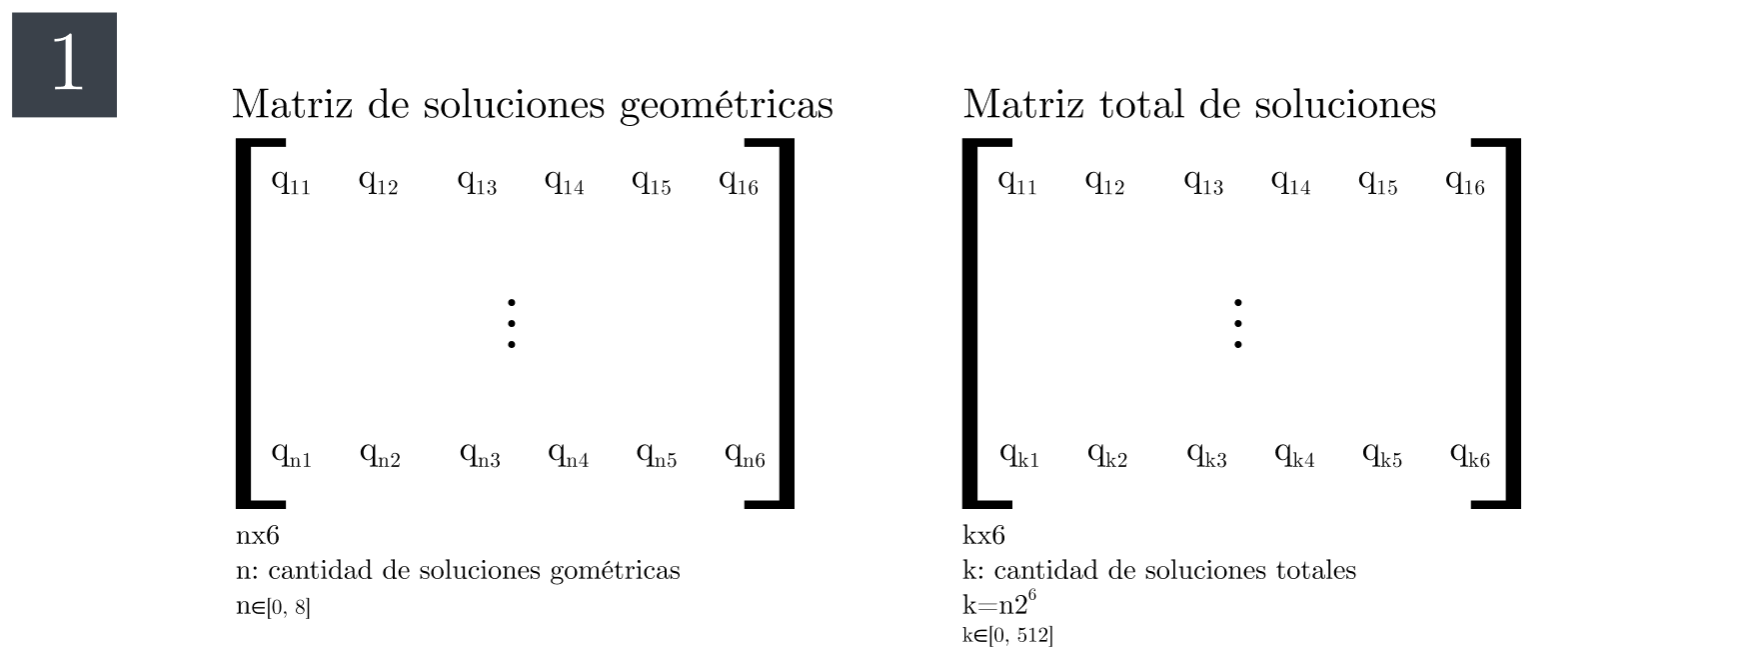
\includegraphics[width=0.85\linewidth]{AMPL_1.png}
    \caption{Matriz de soluciones geométricas y matriz total de soluciones}
    \label{fig:ampl_1}
\end{figure}

\begin{figure}[H]
    \centering
    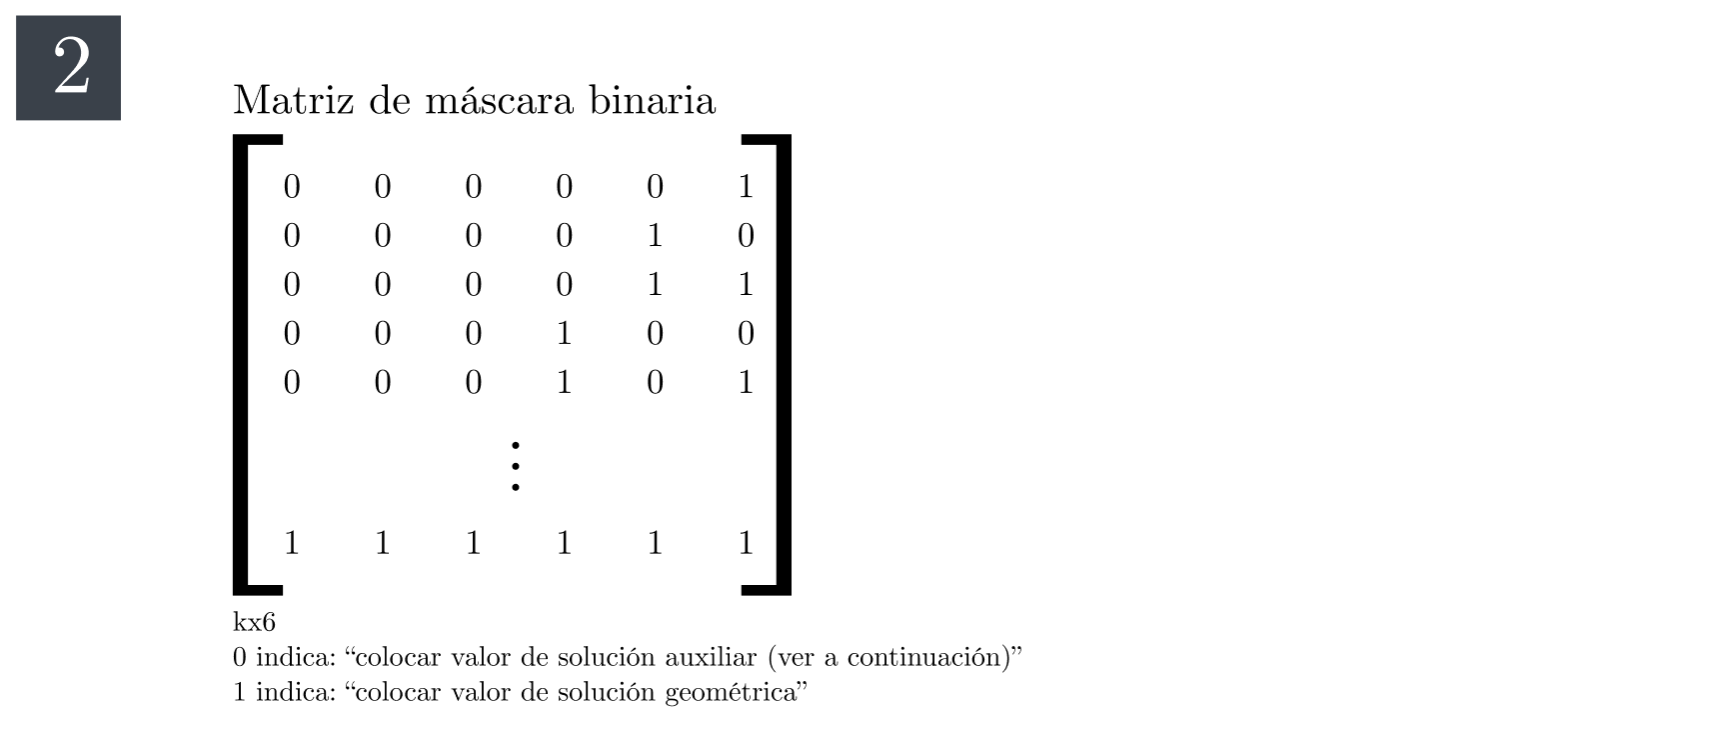
\includegraphics[width=0.85\linewidth]{AMPL_2.png}
    \caption{Matriz de máscara binaria}
    \label{fig:ampl_2}
\end{figure}

\begin{figure}[H]
    \centering
    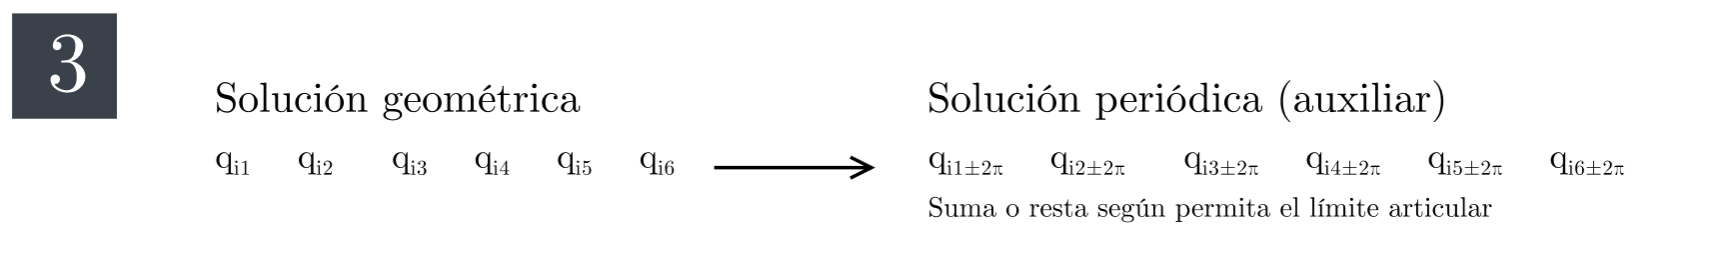
\includegraphics[width=0.85\linewidth]{AMPL_3.png}
    \caption{Solución geométrica genérica y cálculo de solución periódica correspondiente }
    \label{fig:ampl_3}
\end{figure}

La verificación de funcionamiento de la cinemática inversa se explica en \ref{ap:IK}.

% ======================================================================
\subsection{Análisis de singularidades}
\label{sec:analisis_singularidades}

Las singularidades representan configuraciones en las que un manipulador robótico pierde uno o más grados de libertad en el espacio cartesiano, independientemente del movimiento que se imponga en el espacio articular. 
En un robot de seis grados de libertad, estas configuraciones se identifican a partir del análisis del Jacobiano geométrico $\mathbf{J}(\mathbf{q})$, cuya pérdida de rango completo indica la presencia de una singularidad. Formalmente, una configuración $\mathbf{q} \in \mathbb{R}^6$ es singular si y solo si

\begin{equation}
    \det\bigl(\mathbf{J}(\mathbf{q})\bigr) = 0.
\end{equation}

En estas configuraciones, el robot exhibe dos consecuencias prácticas críticas: la imposibilidad de generar velocidades cartesianas en determinadas direcciones y la amplificación teóricamente ilimitada de velocidades articulares ante pequeñas velocidades cartesianas en las direcciones próximas al espacio nulo del Jacobiano. Por este motivo, la detección y el tratamiento de singularidades son requisitos indispensables en la planificación de trayectorias y en el control de manipuladores industriales.


Al realizar un análisis geométrico, se identifican tres tipos de 
singularidades: de hombro, de codo y de muñeca. Matemáticamente, 
cada una corresponde a una condición específica sobre las variables 
articulares del robot.

\begin{itemize}
    \item \textbf{Singularidad de muñeca:} ocurre cuando el eje de la 
    articulación 4 y el eje de la articulación 6 se alinean, colapsando 
    un grado de libertad en la orientación del efector final. La condición 
    que la define es
    \begin{equation}
        q_5 = k\pi, \qquad k \in \mathbb{Z}.
    \end{equation}

    \item \textbf{Singularidad de codo:} ocurre cuando los ejes de las 
    articulaciones 2 y 4 se alinean, de modo que ambas articulaciones 
    producen el mismo efecto rotacional y el Jacobiano pierde rango. 
    La condición que la define es
    \begin{equation}
        q_3 = k\pi, \qquad k \in \mathbb{Z}.
    \end{equation}

    \item \textbf{Singularidad de hombro:} ocurre cuando el punto de intersección de los ejes articulares 5 y 6 se encuentra sobre el plano que forman los ejes articulares 1 y 2. La forma analítica de esta explicación es hacer que la proyección vertical total de \textit{a2, a3 y d5} sea nula:
    \begin{equation}
        a_2\sin(q_2)+a_3\sin(q_2+q_3)+d_5\sin(q_2+q_3+q_4)=0
    \end{equation}
    
\end{itemize}

La verificación de las singularidades se explica en \ref{ap:SINGULARIDADES}

% ======================================================================
\newpage
\section{Planificación de trayectorias}
\label{sec:planificacion_trayectorias}

%
% ============
%
\subsection{Generación de trayectorias}
\label{sec:generacion_trayectorias}

La generación de trayectorias constituye una etapa fundamental en el control de manipuladores robóticos, ya que permite definir la evolución temporal de las variables articulares o del efector final entre configuraciones iniciales y finales previamente establecidas. Este proceso no solo implica determinar el camino geométrico a seguir, sino también garantizar que el movimiento cumpla con restricciones físicas del sistema, tales como límites de velocidad, aceleración y suavidad.

El cálculo de la trayectoria se realiza dentro del script \colorbox{gray!20}{\texttt{gen\_traj.m}} el cual recibe los siguientes argumentos:
\begin{itemize}
    \item \textbf{R}: definición del robot.
    \item \textbf{cpoints\_input}: matriz de puntos vía en coordenadas cartesianas, uno por fila, con una séptima columna que indica el modo de interpolación para llegar a ese punto (0: espacio articular, 1: espacio cartesiano).
    \item \textbf{q0}: coordenada articular inicial del robot.
    \item \textbf{qdmax, qddmax}: velocidades y aceleraciones máximas articulares.
    \item \textbf{verbose}: controla la verbosidad de la cinemática inversa interna.
    \item \textbf{vmax, amax, wmax, alphamax}: velocidades y aceleraciones lineales y angulares máximas del efector final.
\end{itemize}

El trabajo comienza por analizar la séptima columna de cada fila (punto vía) del argumento \textbf{cpoints\_input}, para determinar en qué modo de interpolación llegar a ese punto: 0 para interpolación en espacio articular y 1 para interpolación en espacio cartesiano.

Si el modo es 0, el primer paso es empaquetar todos los puntos vías consecutivos dentro de la matriz de \textit{waypoints} para obtener una trayectoria suave y continua sin detención en cada punto vía dado originalmente. En segundo lugar, estos puntos se transforman al espacio articular mediante la aplicación del cálculo analítico de la cinemática inversa provisto en el script \colorbox{gray!20}{\texttt{inv\_kinematics.m}}. Los puntos vía en el espacio articular son enviados al interpolador de espacio articular provisto por el toolbox \textbf{mstraj}. 

En el otro caso, cuando el modo es 1, la interpolación se da en el espacio cartesiano por lo que simplemente se envía el punto objetivo al interpolador en espacio cartesiano provisto en el toolbox \textit{ctraj} en conjunto con la ley de movimiento definida en \textit{s}. La ley de movimiento se calcula de modo que el tiempo total del movimiento quede definido por el parámetro más comprometido (vmax, amax, wmax, alphamax). 

En ambos casos, al calcular la trayectoria, esta se acopla a continuación de la trayectoria ya definida en una matriz. El último elemento de esta matriz se utiliza punto inicial de la siguiente interpolación, en el caso de que esté vacía, es decir, que sea la primera interpolación, se utilizará el argumento \textbf{q0}.

La validación del funcionamiento del módulo de generación de trayectorias se presenta en el Apéndice~\ref{ap:generacion_trayectorias}.

%
% ============
%
\subsection{Escalamiento de velocidades y aceleraciones}
\label{sec:escalamiento_velocidades}

Una vez generada una trayectoria preliminar, es necesario verificar que el perfil de velocidades y aceleraciones resultante respeta los límites cinemáticos del robot, tanto en el espacio articular como en el espacio cartesiano. Para esto se realiza el siguiente procedimiento de dos etapas.

\subsubsection*{Primera etapa: generación preliminar y cómputo del factor de escala}

Se genera la trayectoria con los parámetros nominales. A continuación, la función auxiliar \colorbox{gray!20}{\texttt{compute\_scale}} calcula numéricamente las velocidades y aceleraciones articulares mediante diferencias finitas y, a través del Jacobiano del robot $\mathbf{J}(\mathbf{q})$, obtiene las velocidades y aceleraciones cartesianas:
\begin{equation}
    \mathbf{v} = \mathbf{J}(\mathbf{q})\,\dot{\mathbf{q}}, \qquad
    \mathbf{a} = \mathbf{J}(\mathbf{q})\,\ddot{\mathbf{q}}.
\end{equation}

Con estos valores se determina si algún límite es superado y en qué medida. La clave del método reside en la relación entre el factor de escala temporal $k$ y sus efectos sobre la cinemática: si se ejecuta el mismo recorrido en $k$ veces más tiempo, las velocidades se reducen en un factor $1/k$ y las aceleraciones en $1/k^2$. Por esto, los factores de escala individuales se calculan de forma diferente según se trate de una restricción de velocidad o de aceleración:
\begin{equation}
    k_{\dot{q}} = \max_{i}\frac{|\dot{q}_i|_{\max}}{\dot{q}_{i,\max}}, \qquad
    k_{\ddot{q}} = \sqrt{\max_{i}\frac{|\ddot{q}_i|_{\max}}{\ddot{q}_{i,\max}}},
\end{equation}
y de manera análoga para las magnitudes cartesianas:
\begin{equation}
    k_v = \frac{\|\mathbf{v}\|_{\max}}{v_{\max}}, \quad
    k_\omega = \frac{\|\boldsymbol{\omega}\|_{\max}}{\omega_{\max}}, \quad
    k_a = \sqrt{\frac{\|\mathbf{a}\|_{\max}}{a_{\max}}}, \quad
    k_\alpha = \sqrt{\frac{\|\boldsymbol{\alpha}\|_{\max}}{\alpha_{\max}}}.
\end{equation}

La raíz cuadrada en los factores de aceleración refleja que, al estirar el tiempo por $k$, la aceleración se reduce en $k^2$, por lo que para cancelar una violación de factor $r$ en aceleración basta con $k = \sqrt{r}$. El factor de escala final del segmento es:
\begin{equation}
    k = \max\bigl(1,\; k_{\dot{q}},\; k_{\ddot{q}},\; k_v,\; k_\omega,\; k_a,\; k_\alpha\bigr).
\end{equation}

Si $k = 1$ no existe ninguna violación y la trayectoria preliminar es válida.

\subsubsection*{Segunda etapa: regeneración de la trayectoria}

Si $k > 1$, se regenera la trayectoria con el tiempo extendido. En el caso de interpolación articular (\texttt{mstraj}), esto equivale a reducir los límites de velocidad articular a $\dot{\mathbf{q}}_{\max}/k$ y extender el tiempo de rampa a $t_{\mathrm{acc}} \cdot k$, con lo que la trayectoria resultante cumple todos los límites. En el caso de interpolación cartesiana, simplemente se extiende el tiempo total a $t_f$ a $k \cdot t_f$ y se regenera la ley de movimiento quintic. En este modo existe además una estimación inicial de $t_f$ basada en las propiedades analíticas del perfil quintic empleado, que sirve como punto de partida para la verificación posterior.


El resultado del escalamiento aplicado, incluyendo la comparativa entre los perfiles de velocidad antes y después del proceso tanto en el espacio articular como en el cartesiano, se presenta en el Apéndice~\ref{ap:generacion_trayectorias} (figuras~\ref{fig:verif_gen_traj_vel} y \ref{fig:verif_gen_traj_vel_cart}).





% ======================================================================
\newpage
\section{Diseño y adaptación de CAD}
\label{sec:CAD}

El diseño tridimensional del robot constituye una etapa fundamental para la visualización y validación del modelo cinemático desarrollado. Con este objetivo, se elaboraron los modelos CAD de cada eslabón en el entorno \textit{Fusion 360}, exportándolos posteriormente en formato STL para su integración en el entorno de simulación. Dado que las dimensiones y unidades de los archivos exportados no coinciden directamente con los parámetros del modelo DH, se desarrolló el script \colorbox{gray!20}{\texttt{scale.m}}, que se encarga de escalar cada STL de forma que las dimensiones coincidan con las definidas modelo DH. Adicionalmente, durante el proceso de diseño se buscó maximizar el aprovechamiento del rango articular de cada articulación, procurando que la configuración mecánica permita explotar al máximo las capacidades de movimiento del robot sin incurrir en interferencias geométricas entre sus componentes.

\subsection{Visualización del modelo en MATLAB}

La figura~\ref{fig:robot_matlab_completo} muestra el ensamblaje completo del robot
renderizado en \textit{MATLAB} mediante la toolbox de \textit{Peter Corke}, con los
marcos de referencia DH superpuestos sobre cada eslabón y con transparencia aplicada
sobre las mallas STL, lo que permite verificar visualmente la alineación entre los ejes articulares y la geometría de cada pieza. Se incluyen también los sistemas del modelo Dh.

\begin{figure}[H]
    \centering
    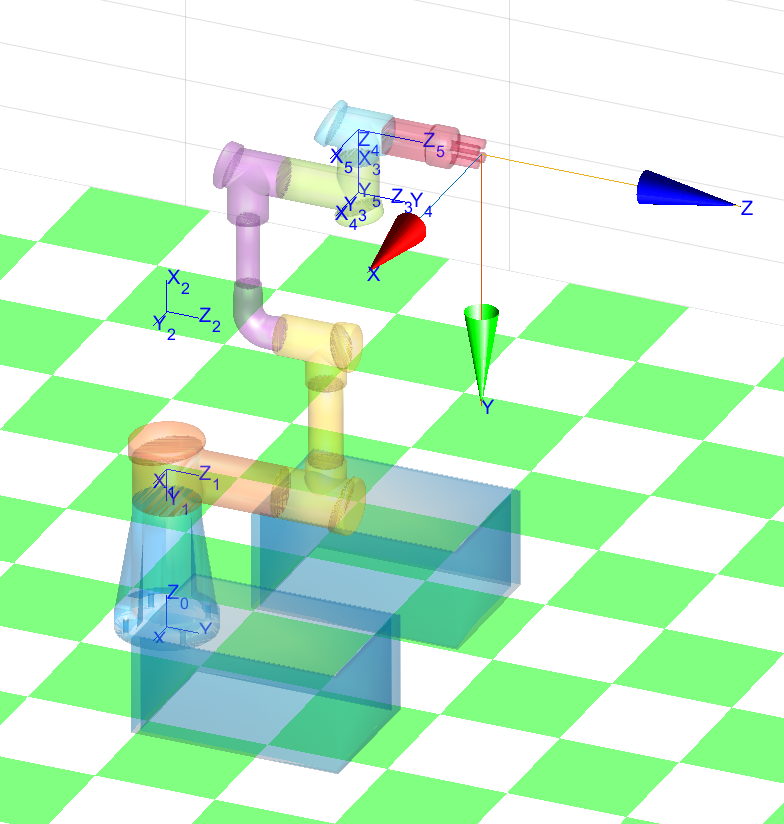
\includegraphics[width=0.75\linewidth]{CAD_ROBOT.png}  
    \caption{Modelo del robot renderizado en \textit{MATLAB} con marcos de referencia DH.}
    \label{fig:robot_matlab_completo}
\end{figure}

\subsection{Diseño de piezas en \textit{Fusion 360}}

A continuación se presentan los modelos de cada pieza diseñada en \textit{Fusion 360}. Para cada componente se detallan las decisiones de diseño adoptadas en relación al aprovechamiento del rango articular y la evitación de interferencias geométricas. En todos los casos, el sistema de referencia de cada cuerpo se adapta de forma que resulte correlativo con el modelo DH, garantizando la coincidencia entre el eje de giro definido en la parametrización cinemática y el cuerpo sobre el cual dicho giro se produce.

\subsubsection{Base}

Para el diseño de la base se tienen en cuenta dos premisas. En primer lugar, se incrementa el grosor en la zona de apoyo con el objetivo de aumentar la estabilidad del conjunto. En segundo lugar, se incorpora una altura suficiente para posicionar al robot por encima de las cajas, tal como lo requiere la tarea descrita en la sección \ref{sec:tarea_especificaciones_robot}.

\begin{figure}[H]
    \centering
    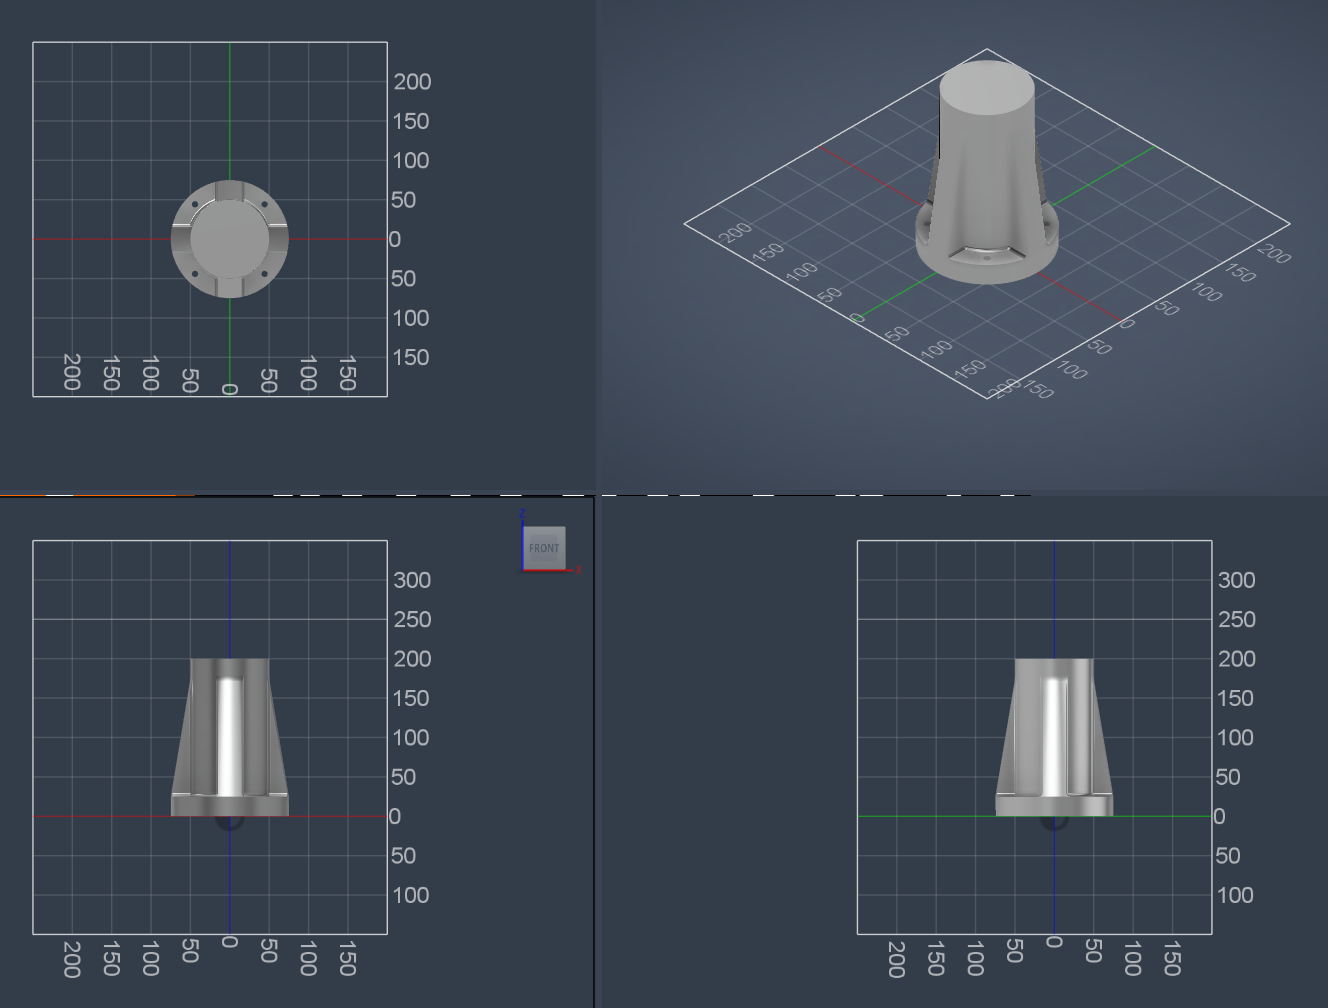
\includegraphics[width=0.75\linewidth]{ESLABON_BASE.png}
    \caption{Diseño de la base en \textit{Fusion 360}.}
    \label{fig:cad_base}
\end{figure}

\subsubsection{Eslabón 1}

El eslabón 1 tiene como objetivo principal proveer una separación del eje central definido por la base, de forma que los eslabones posteriores cuenten con espacio suficiente para aprovechar su rango articular sin incurrir en interferencias geométricas.

\begin{figure}[H]
    \centering
    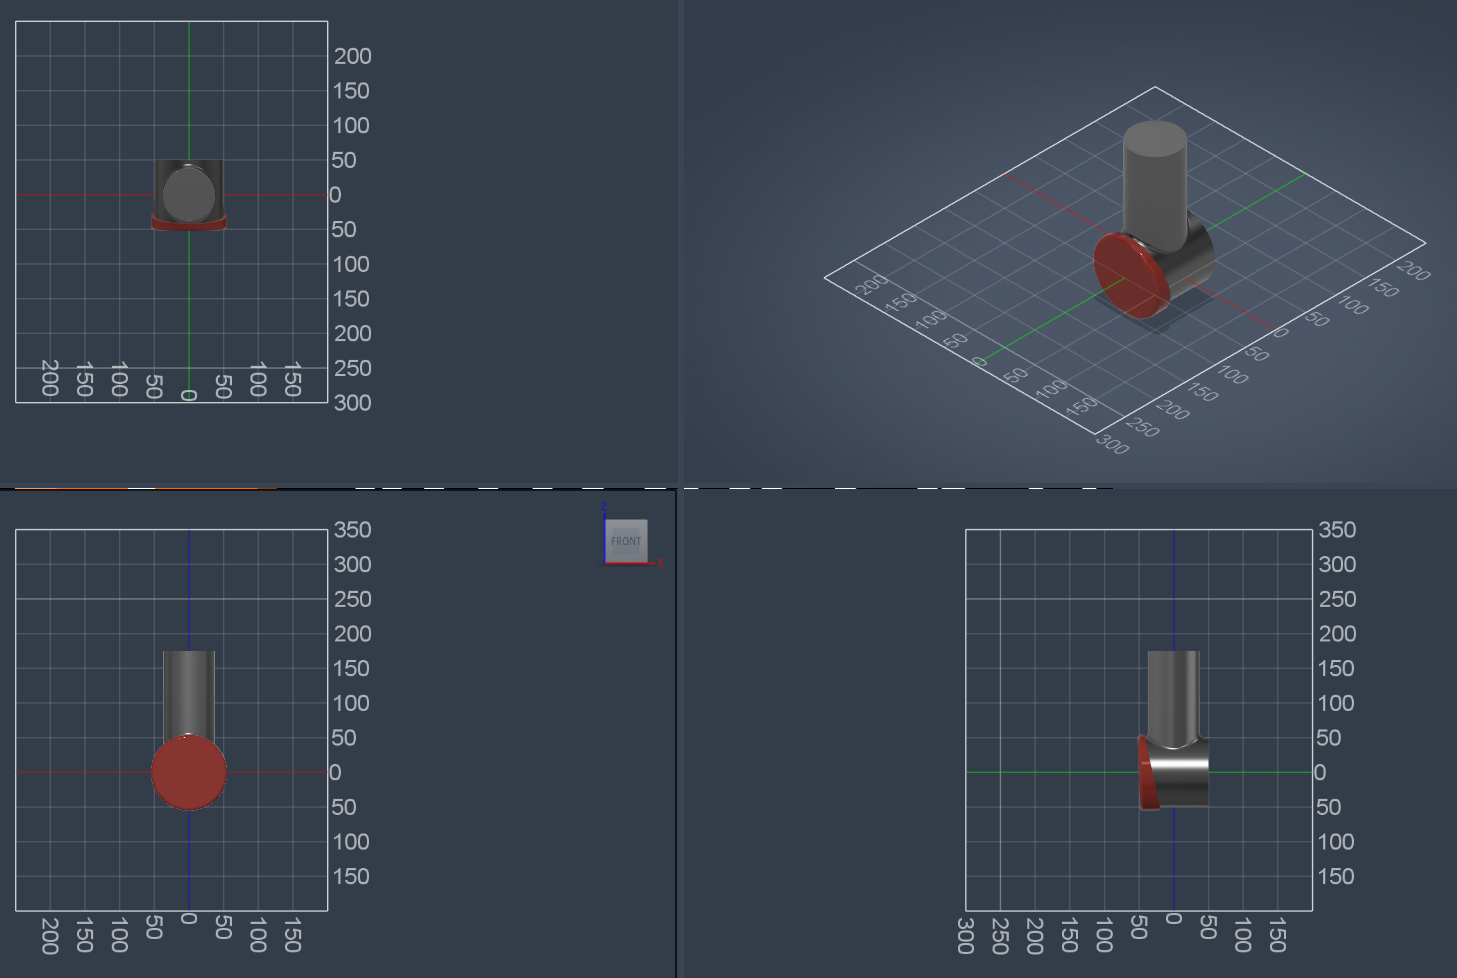
\includegraphics[width=0.75\linewidth]{ESLABON_1.png}
    \caption{Diseño del eslabón 1 en \textit{Fusion 360}.}
    \label{fig:cad_eslabon1}
\end{figure}

\subsubsection{Eslabón 2}

El eslabón 2 cumple la misma función que el eslabón 1. La separación total requerida se distribuye entre ambos eslabones, logrando un equilibrio en la geometría del robot.

\begin{figure}[H]
    \centering
    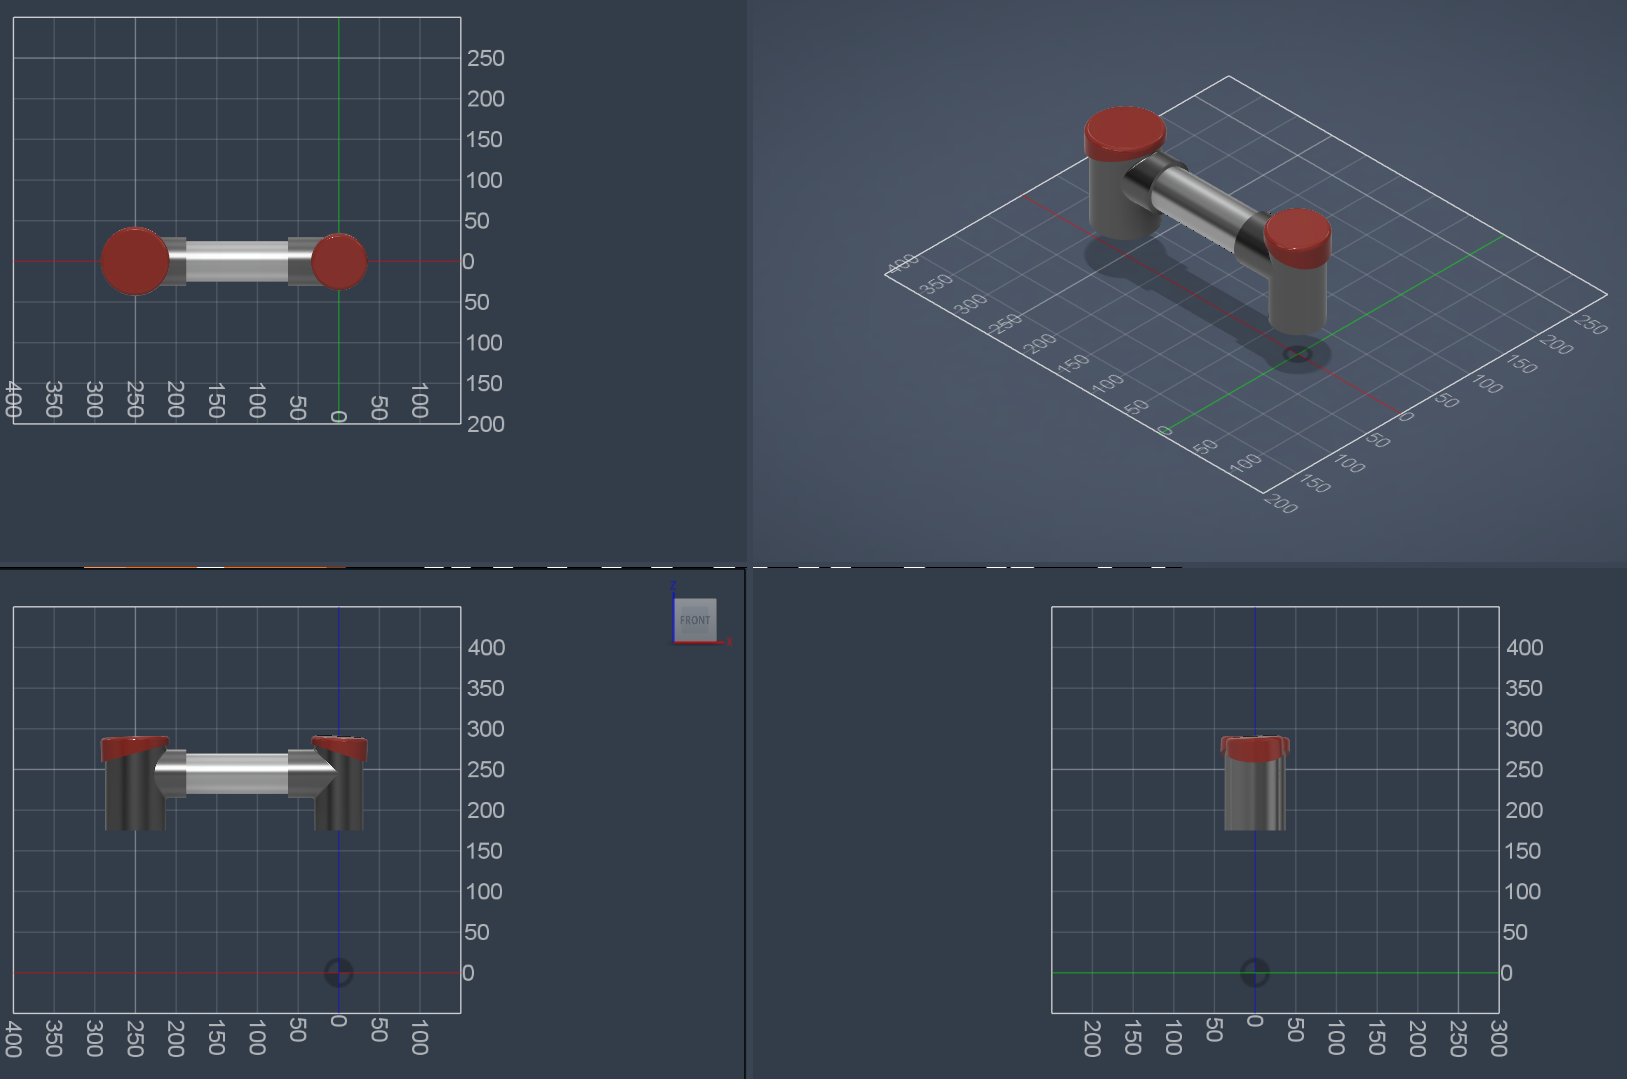
\includegraphics[width=0.75\linewidth]{ESLABON_2.png}
    \caption{Diseño del eslabón 2 en \textit{Fusion 360}.}
    \label{fig:cad_eslabon2}
\end{figure}

\subsubsection{Eslabón 3}

El eslabón 3 no presenta decisiones de diseño particulares más allá de las consideraciones generales de la sección.

\begin{figure}[H]
    \centering
    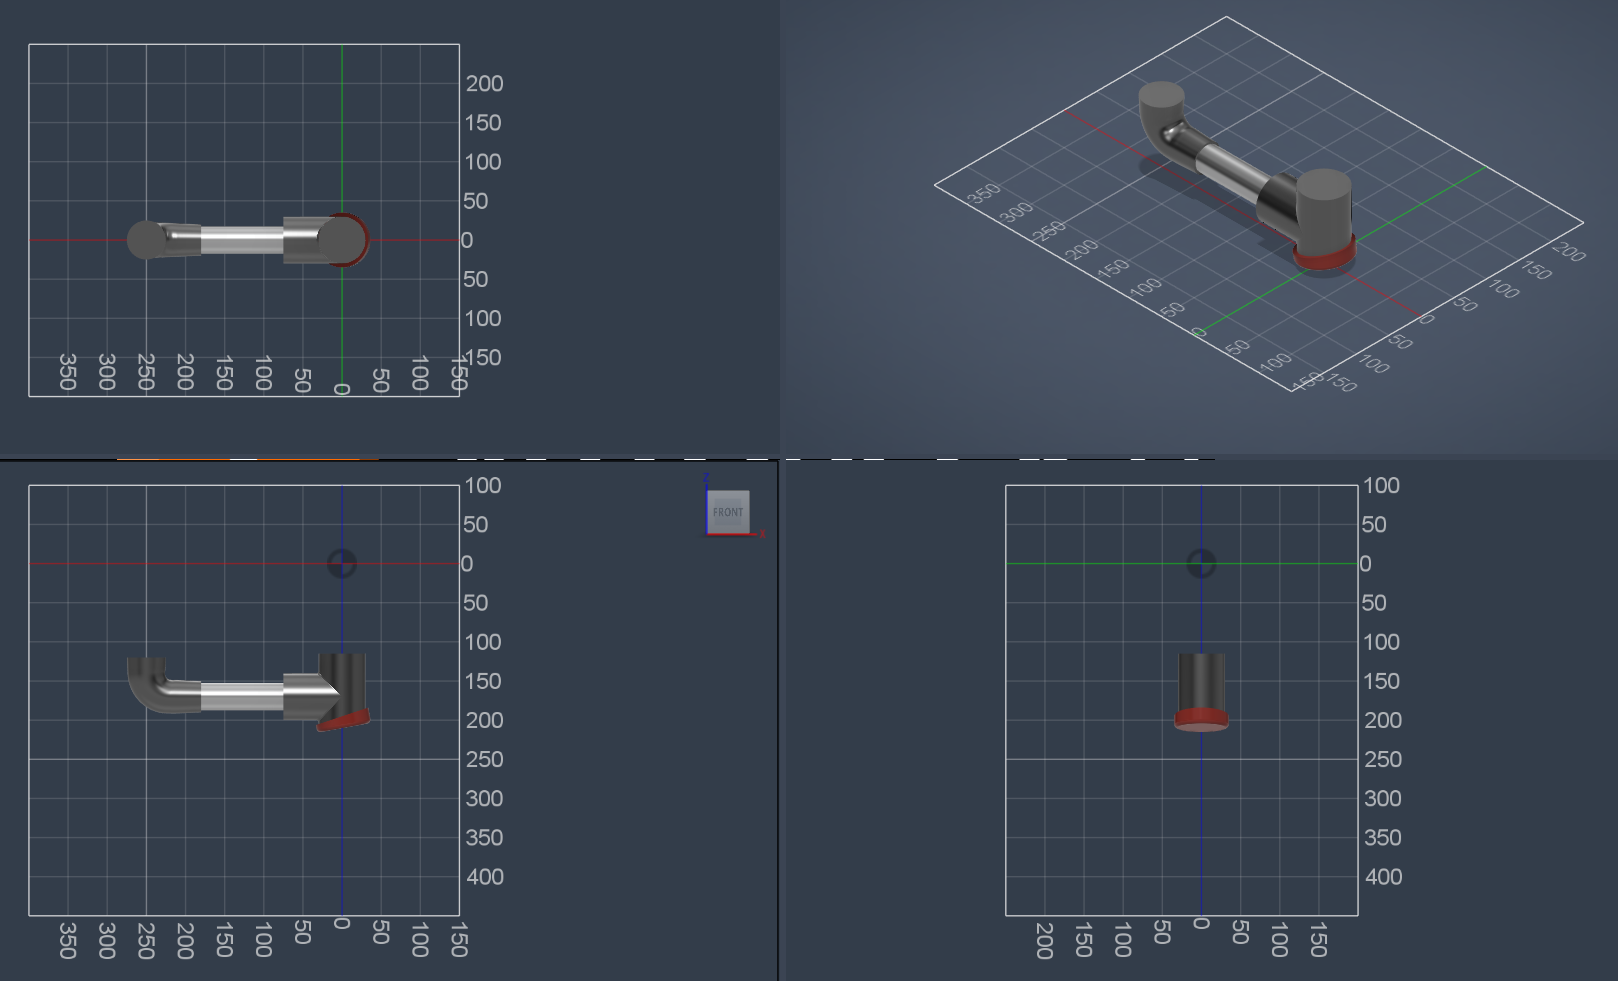
\includegraphics[width=0.75\linewidth]{ESLABON_3.png}
    \caption{Diseño del eslabón 3 en \textit{Fusion 360}.}
    \label{fig:cad_eslabon3}
\end{figure}

\subsubsection{Eslabón 4}

El eslabón 4 no presenta decisiones de diseño particulares más allá de las consideraciones generales de la sección.

\begin{figure}[H]
    \centering
    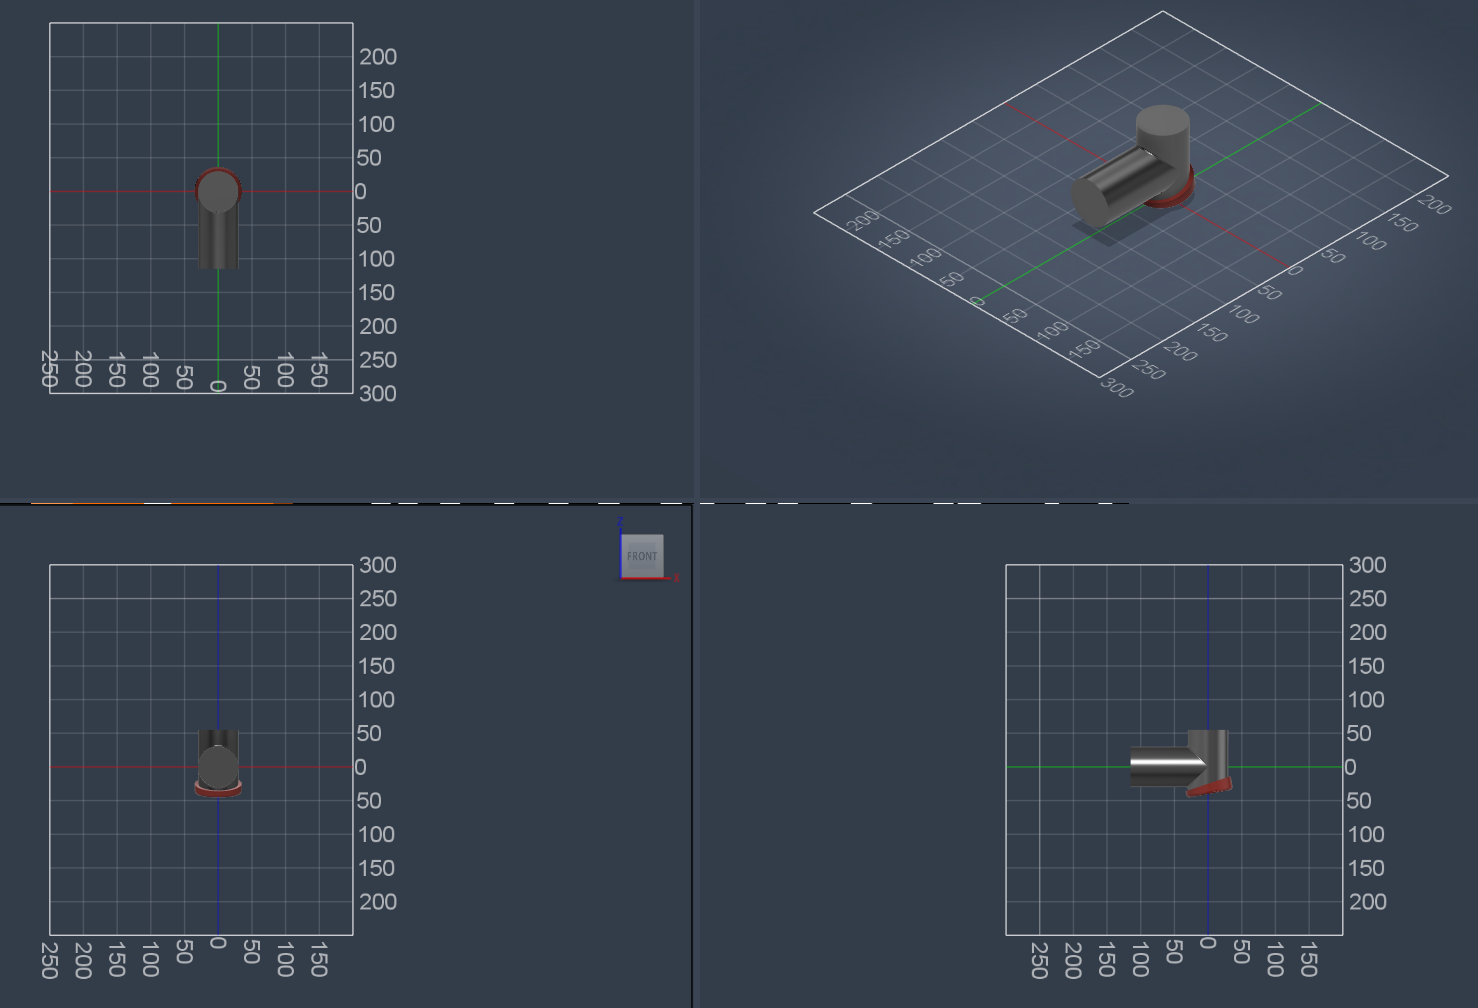
\includegraphics[width=0.75\linewidth]{ESLABON_4.png}
    \caption{Diseño del eslabón 4 en \textit{Fusion 360}.}
    \label{fig:cad_eslabon4}
\end{figure}

\subsubsection{Eslabón 5}

El eslabón 5 no presenta decisiones de diseño particulares más allá de las consideraciones generales de la sección.

\begin{figure}[H]
    \centering
    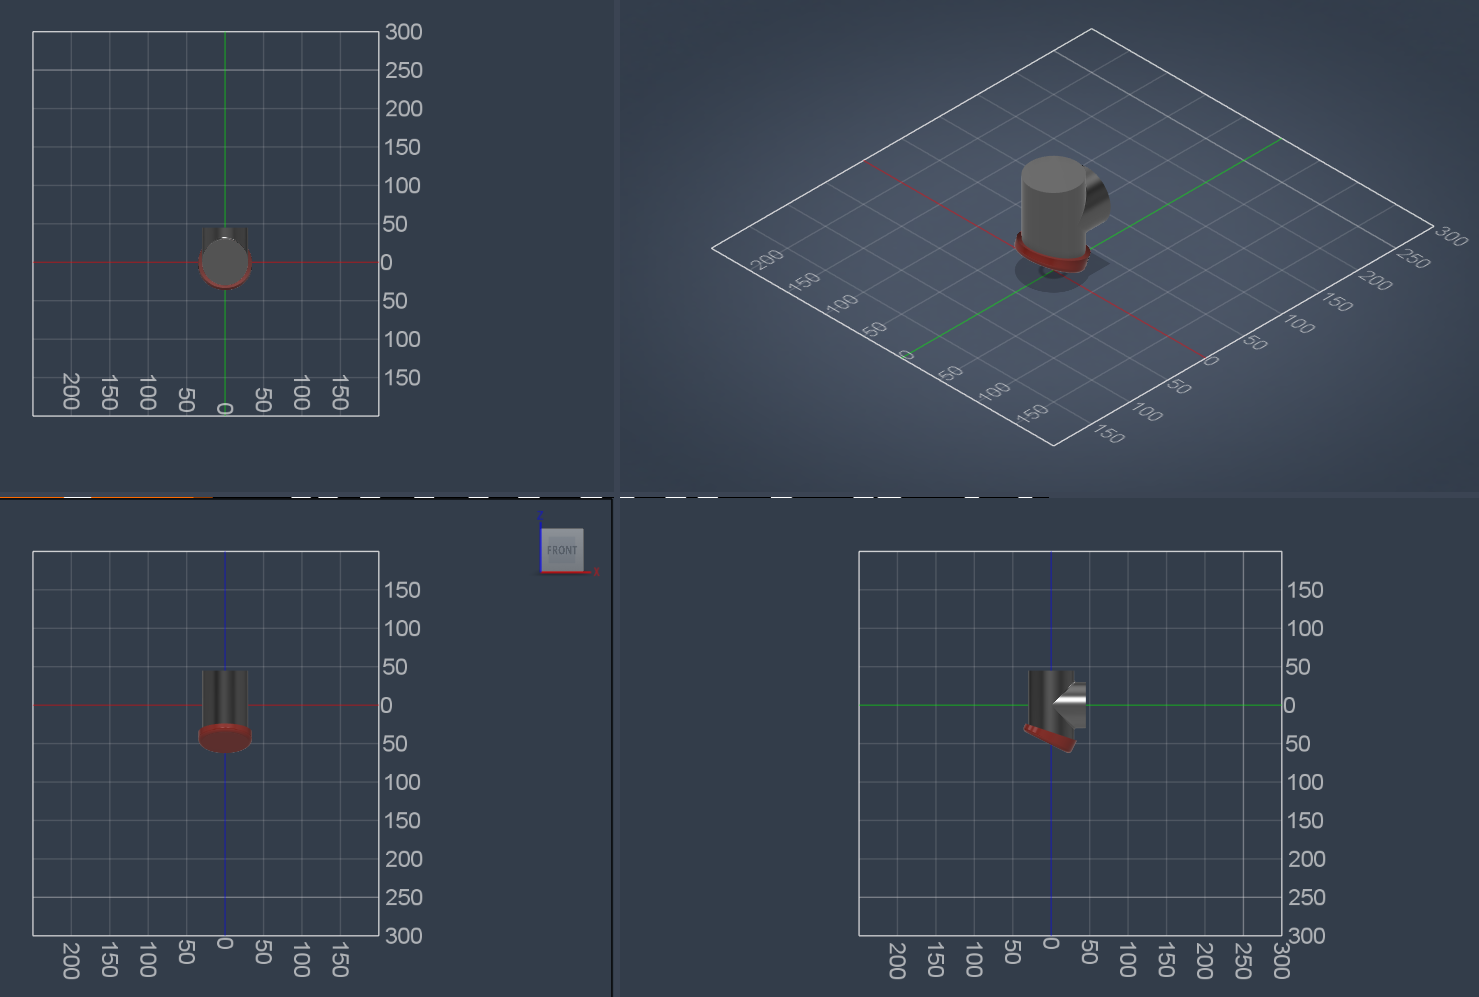
\includegraphics[width=0.75\linewidth]{ESLABON_5.png}
    \caption{Diseño del eslabón 5 en \textit{Fusion 360}.}
    \label{fig:cad_eslabon5}
\end{figure}

\subsubsection{Eslabón 6 ---Herramienta}

El eslabón 6 corresponde a la herramienta del sistema y no presenta decisiones de diseño particulares más allá de las consideraciones generales de la sección.

\begin{figure}[H]
    \centering
    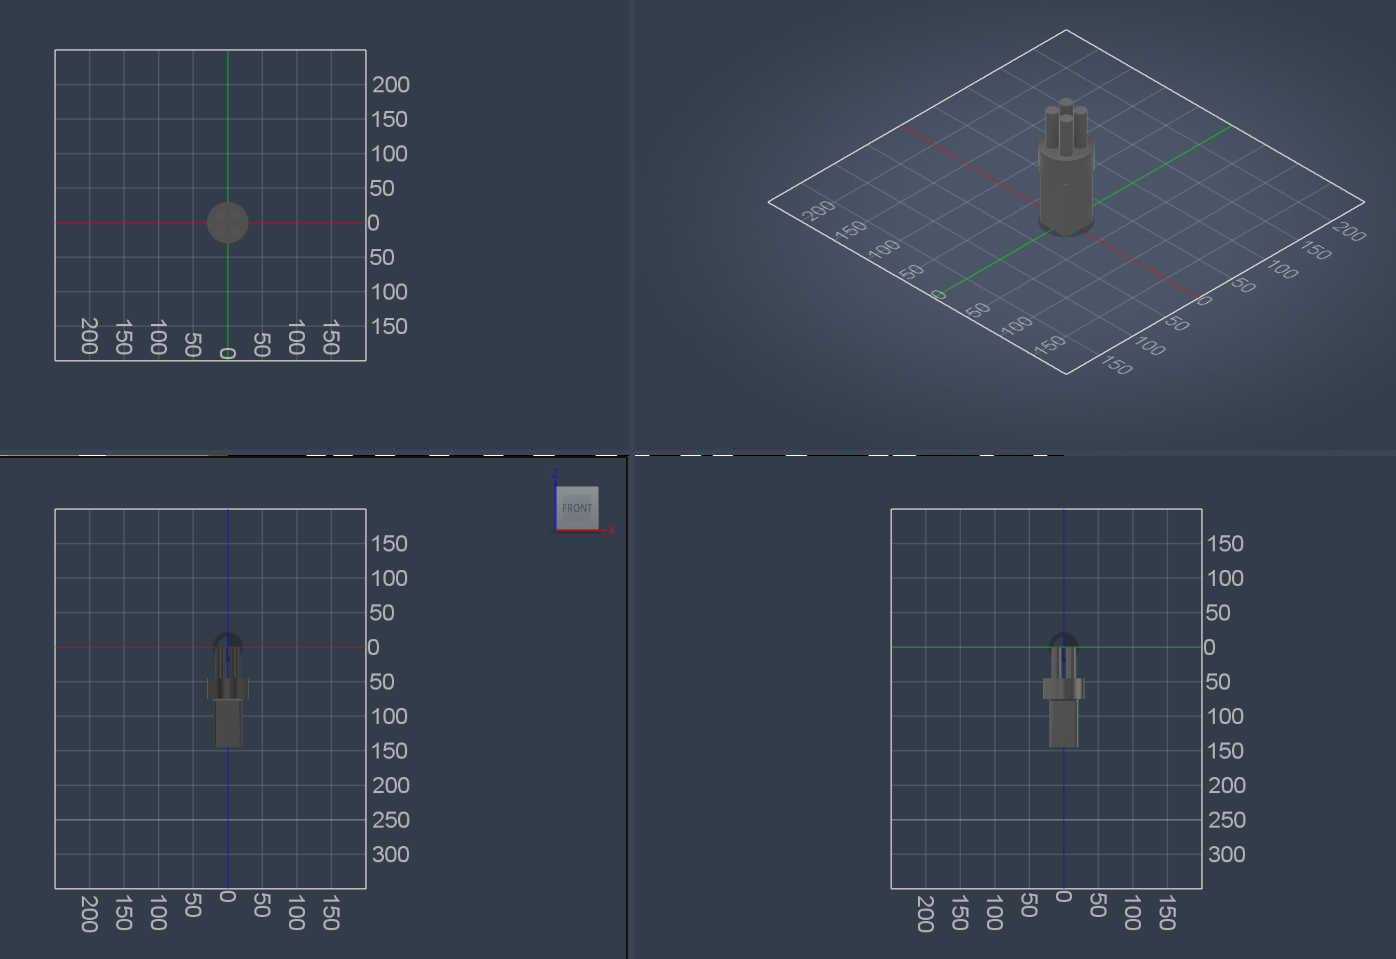
\includegraphics[width=0.75\linewidth]{ESLABON_6.png}
    \caption{Diseño del eslabón 6 (herramienta) en \textit{Fusion 360}.}
    \label{fig:cad_eslabon6}
\end{figure}

\subsection{Diseño alternativo: apertura unidireccional de eslabones}

En robots de morfología similar al \href{https://www.universal-robots.com/products/ur3e?utm_source=chatgpt.com}{UR3e}, los eslabones se disponen de manera tal que, visto desde el plano lateral, el brazo adopta una forma en \textit{Z}: el eslabón 2 se extiende en un sentido y el eslabón 3 se pliega en sentido opuesto, de forma que los giros de ambas articulaciones se compensan parcialmente entre sí. Esto implica que el aprovechamiento del rango articular de cada junta no es aditivo en la dirección de extensión del brazo.

Como alternativa, se diseñó una segunda versión del robot en la que todos los eslabones se abren en el mismo sentido de giro, adoptando una morfología en \textit{C} vista desde el plano lateral. De este modo, el aporte de cada articulación al alcance del efector final es aditivo, lo que permite un mejor aprovechamiento del rango articular disponible.

Cabe destacar que esta modificación es estrictamente geométrica: la parametrización cinemática del robot no varía, dado que la definición del modelo Denavit-Hartenberg depende de la disposición de los ejes articulares y no de la forma particular de los eslabones. En consecuencia, toda la cinemática directa e inversa desarrollada en la sección \ref{sec:cinematica} es igualmente válida para ambos diseños.

\begin{figure}[H]
    \centering
    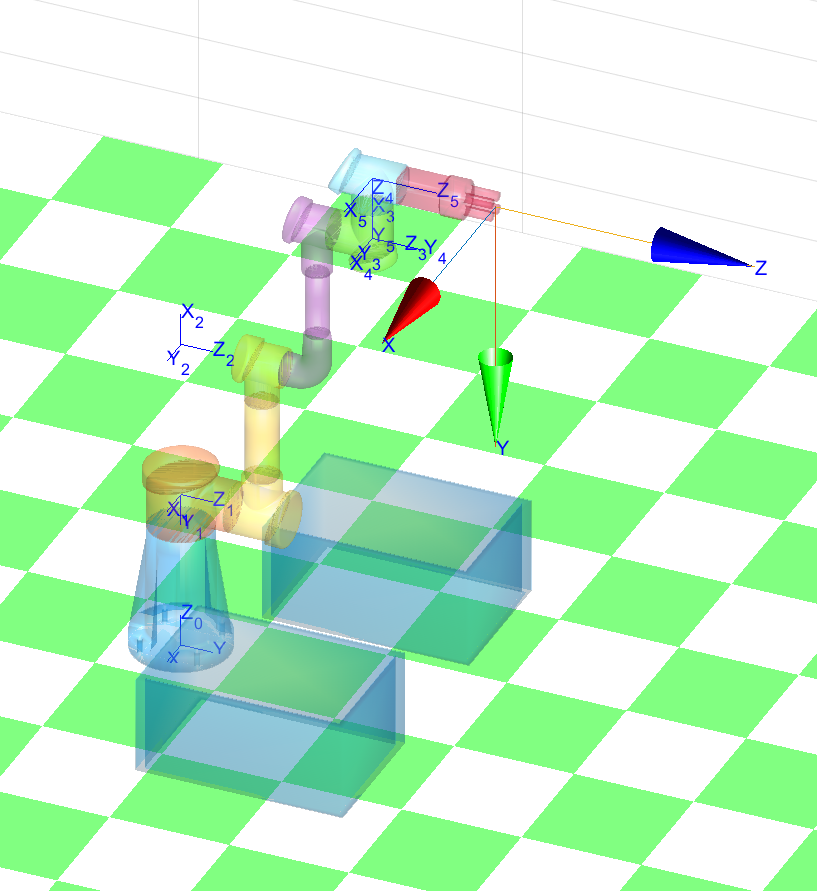
\includegraphics[width=0.75\linewidth]{CAD_ROBOT_ALT.png}
    \caption{Modelo del robot con diseño alternativo de apertura unidireccional renderizado en \textit{MATLAB}.}
    \label{fig:cad_robot_alt}
\end{figure}



% ======================================================================
\newpage
\section{Simulación y verificación de tarea}
\label{sec:sim_tarea}

Implementando, de forma conjunta el cálculo de la cinemática inversa y el algoritmo de generación de trayectorias, puede desarrollarse una trayectoria para la tarea la cual luego será simulada y analizada.

Para esto se definen los siguientes puntos vía, cuyas orientaciones corresponden a ángulos de Euler ZYX en grados (la herramienta apunta siempre hacia abajo, $\beta = 180\degree$):

\begin{table}[H]
    \centering
    \label{tab:puntos_via}
    \renewcommand{\arraystretch}{1.3}
    \begin{tabular}{lrrrrrr}
        \toprule
        \textbf{Punto} & \textbf{x [m]} & \textbf{y [m]} & \textbf{z [m]} & \boldmath$\alpha$ [\degree] & \boldmath$\beta$ [\degree] & \boldmath$\gamma$ [\degree] \\
        \midrule
        \texttt{caja\_origen\_superior}  & $-0.22$ & $0.30$ & $0.20$ & $0$ & $180$ & $0$ \\
        \texttt{caja\_origen\_inferior}  & $-0.22$ & $0.30$ & $0.01$ & $0$ & $180$ & $0$ \\
        \texttt{aux\_1}                  & $-0.10$ & $0.30$ & $0.22$ & $0$ & $180$ & $0$ \\
        \texttt{punto\_medio}            & $ 0.00$ & $0.30$ & $0.25$ & $0$ & $180$ & $0$ \\
        \texttt{aux\_2}                  & $ 0.10$ & $0.30$ & $0.22$ & $0$ & $180$ & $0$ \\
        \texttt{caja\_destino\_superior} & $ 0.22$ & $0.30$ & $0.20$ & $0$ & $180$ & $0$ \\
        \texttt{caja\_destino\_inferior} & $ 0.22$ & $0.30$ & $0.01$ & $0$ & $180$ & $0$ \\
        \bottomrule
    \end{tabular}
    \caption{Puntos vía de la tarea de \textit{bin-to-bin transfer}.}
\end{table}

\text{NOTA:} En el código se realiza la conversión de grados a radianes y, a los valores angulares, se le aplica una pequeña rotación adicional para evitar definir puntos vía que conduzcan a configuraciones singulares.

El \textit{script} permite el comienzo desde un punto aleatorio o desde un punto conocido. Se recuerda que, en conjunto con los puntos vías debe ser proporcionada la indicación del método de interpolación a utilizar, la secuencia es la siguiente:

\begin{enumerate}
    \item \textbf{Posición inicial a punto medio:} Interpolación articular
    \item \textbf{Punto medio a caja origen superior:} Interpolación articular
    \item \textbf{caja origen superior a caja origen inferior:} Interpolación cartesiana
    \item \textbf{Caja origen inferior a caja origen superior:} Interpolación cartesiana
    \item \textbf{Caja origen superior a punto medio:} Interpolación articular
    \item \textbf{Punto medio a caja destino superior:} Interpolación articular
    \item \textbf{Caja destino superior a caja destino inferior:} Interpolación cartesiana
    \item \textbf{Caja destino inferior a caja destino superior:} Interpolación cartesiana
    \item \textbf{Caja destino superior a punto medio:} Interpolación articular
\end{enumerate}

De este modo, se tendrá mayor control en el espacio cartesiano cuando se requiera ingresar y egresar de la caja de recogida y de colocación.

A continuación, se presenta una imagen luego de la simulación:

\begin{figure}[H]
    \centering
    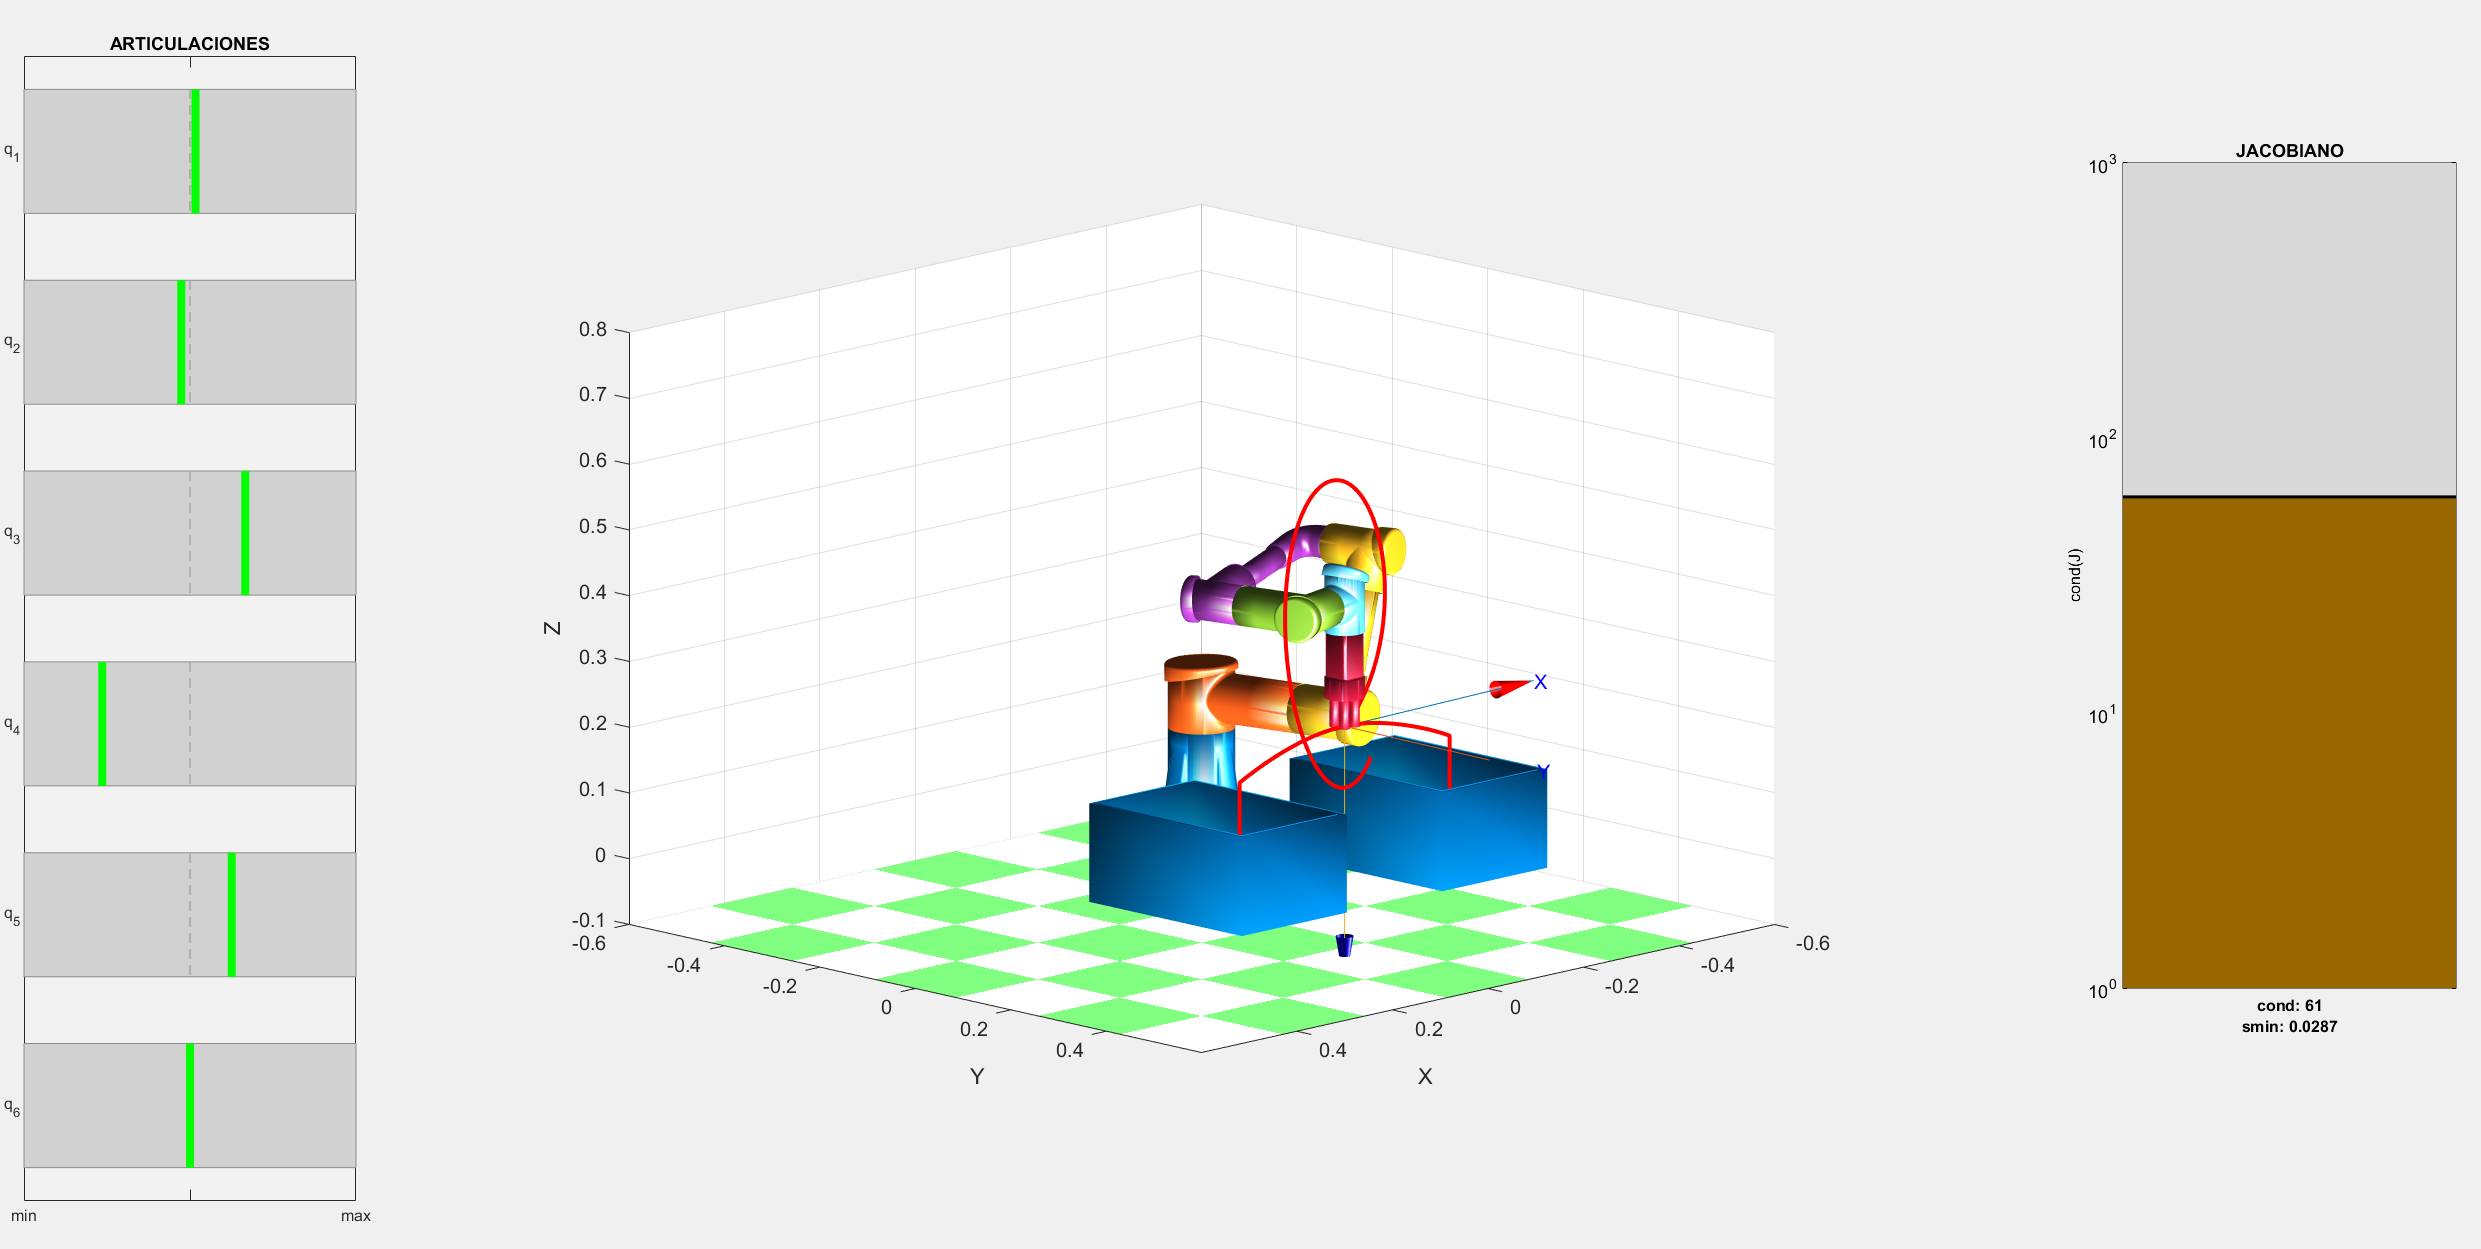
\includegraphics[width=0.85\linewidth]{simulacion_tarea.png}
    \caption{Imagen del final de la simulacion de la tarea.}
    \label{fig:simulacion_tarea}
\end{figure}

En la imagen puede verse el recorrido del robot, el cual ha dejado una traza roja de la posición del efector final. En el inicio de la trayectoria puede verse una maniobra que busca posicionar al robot en el llamado punto medio bajo una configuración articular geométrica lo que beneficiará el comportamiento posterior dado que se comenzará lejos de los límites articulares.
A los costados del robot pueden verse gráficas animadas: a la izquierda, la posición instantánea de cada articulación, y a la derecha, el valor instantáneo del jacobiano, lo que permitiría evaluar posibles mejoras en la trayectoria generada.

Luego de la simulación, se obtienen las siguientes gráficas para el análisis de las variables cinemáticas tanto del efector final como de las articulaciones, puede notarse que no se sobrepasan significativamente límites cinemáticos:

\begin{figure}[H]
    \centering
    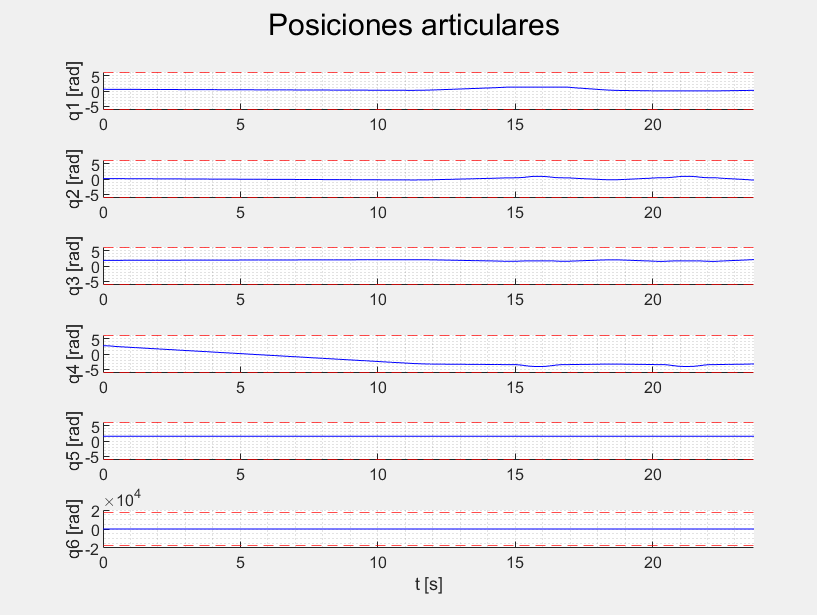
\includegraphics[width=0.85\linewidth]{tarea_pa.png}
    \caption{Evolución de posiciones articulares en la simulacion de la tarea.}
    \label{fig:tarea_pa}
\end{figure}
\begin{figure}[H]
    \centering
    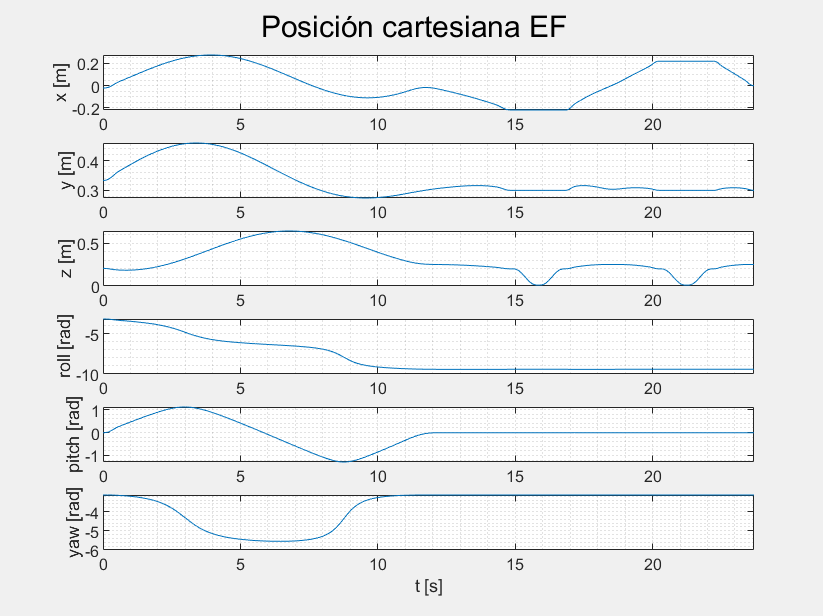
\includegraphics[width=0.85\linewidth]{tarea_pc.png}
    \caption{Evolución de la posición cartesiana del efector final en la simulacion de la tarea.}
    \label{fig:tarea_pc}
\end{figure}
\begin{figure}[H]
    \centering
    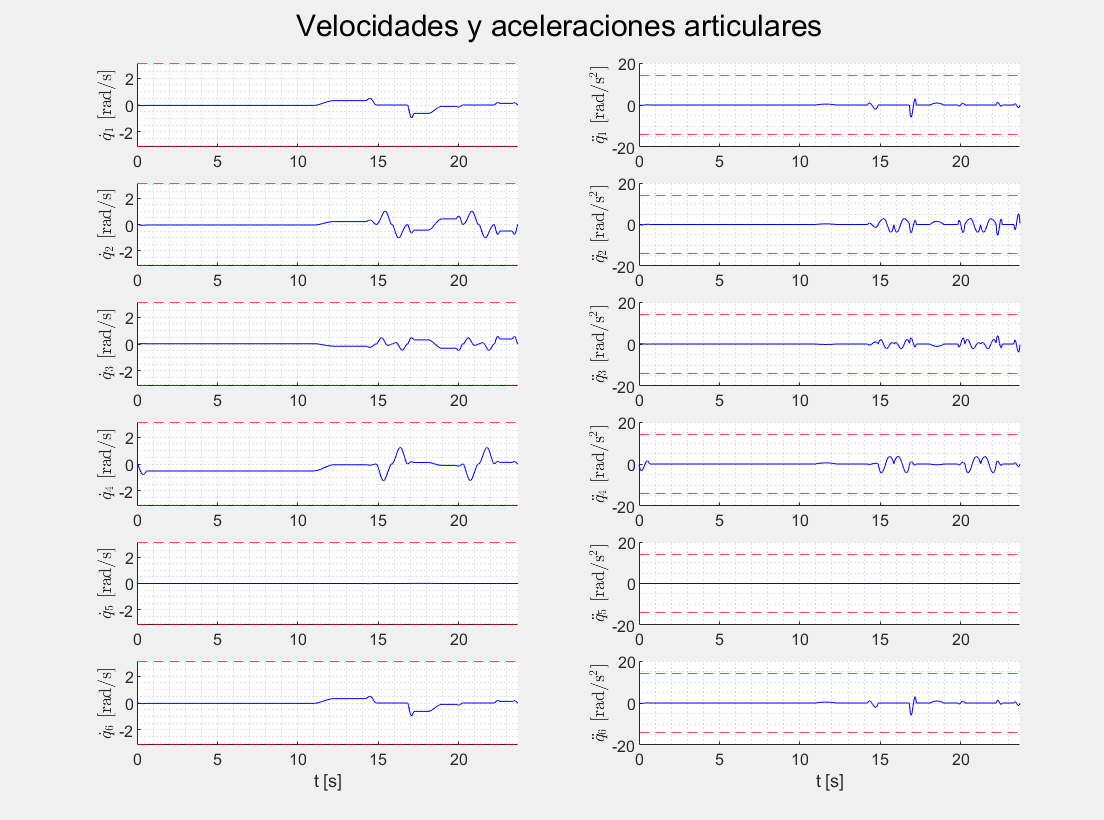
\includegraphics[width=0.85\linewidth]{tarea_va_art.png}
    \caption{Evolución de velocidades y aceleraciones articulares en la simulación de la tarea.}
    \label{fig:tarea_va_art}
\end{figure}
\begin{figure}[H]
    \centering
    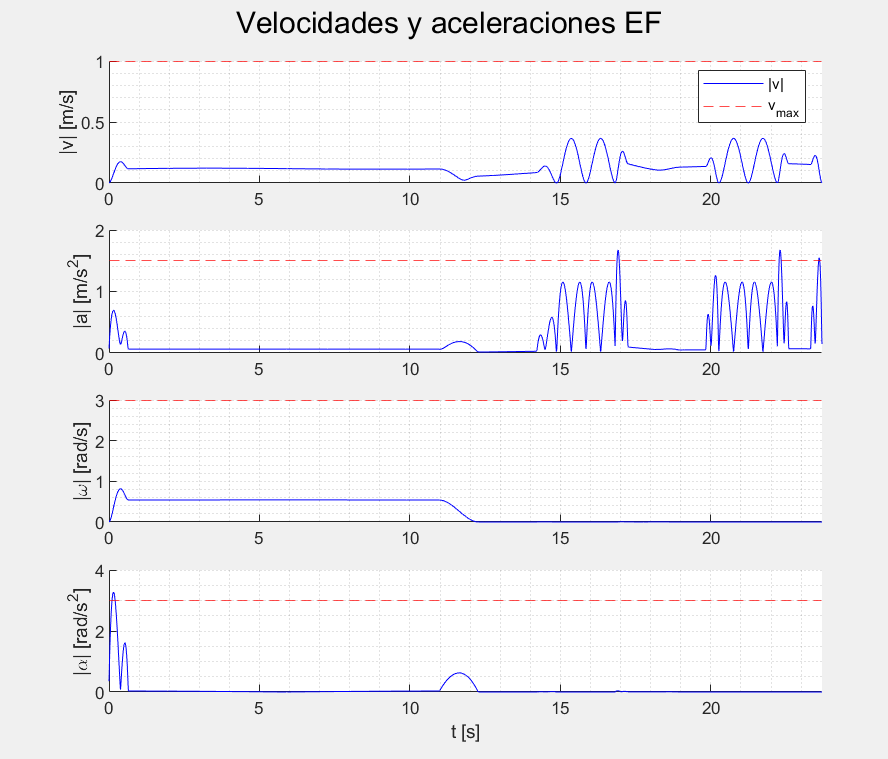
\includegraphics[width=0.85\linewidth]{tarea_va_ef.png}
    \caption{Evolución de velocidades y aceleraciones lineales y angulares del efector final en la simulación de la tarea.}
    \label{fig:tarea_va_ef}
\end{figure}





% ======================================================================
\newpage
\section{Integración en entorno ROS2}
\label{sec:ROS2}

En esta sección se describe la integración del manipulador en el entorno \textit{Robot Operating System 2} (ROS~2). El objetivo es trasladar el desarrollo realizado en MATLAB ---cinemática directa, cinemática inversa y generación de trayectorias--- a una plataforma de software orientada a sistemas robóticos reales, aportando modularidad, comunicación entre procesos y capacidad de simulación mediante RViz. La totalidad del software ha sido desarrollada de forma propia, sin recurrir a librerías de alto nivel específicas de robótica, con el objetivo de maximizar el aprendizaje obtenido y obtener la mayor flexibilidad posible en el diseño de la arquitectura.

La integración se estructura en torno a un conjunto de nodos que encapsulan responsabilidades bien definidas: cálculo cinemático, gestión de trayectorias, \textit{teaching} y visualización a través de una interfaz gráfica. Estos nodos se comunican mediante tópicos y servicios de ROS2, conformando una arquitectura distribuida que permite operar el robot de forma manual o autónoma.

El modelo del robot se describe en formato URDF (\textit{Unified Robot Description Format}), derivado directamente de la parametrización Denavit-Hartenberg definida en la sección \ref{sec:modelado_cinematico}, lo que garantiza consistencia geométrica entre el modelo cinemático y su representación en el entorno de simulación.

\subsection{Arquitectura del sistema}
En primer lugar, se ha desarrollado un nodo \colorbox{gray!20}{\texttt{dr.launcher.py}} que se encarga de levantar todos los nodos y enviar, en la mayoría de los casos, los parámetros del robot \colorbox{gray!20}{\texttt{robot\_params.yml}} el cual, no contiene la definición URDF del robot sino parámetros de la cadena cinemáticos, límites cinemáticos y transformaciones de base y de herramienta.

\begin{figure}[H]
    \centering
    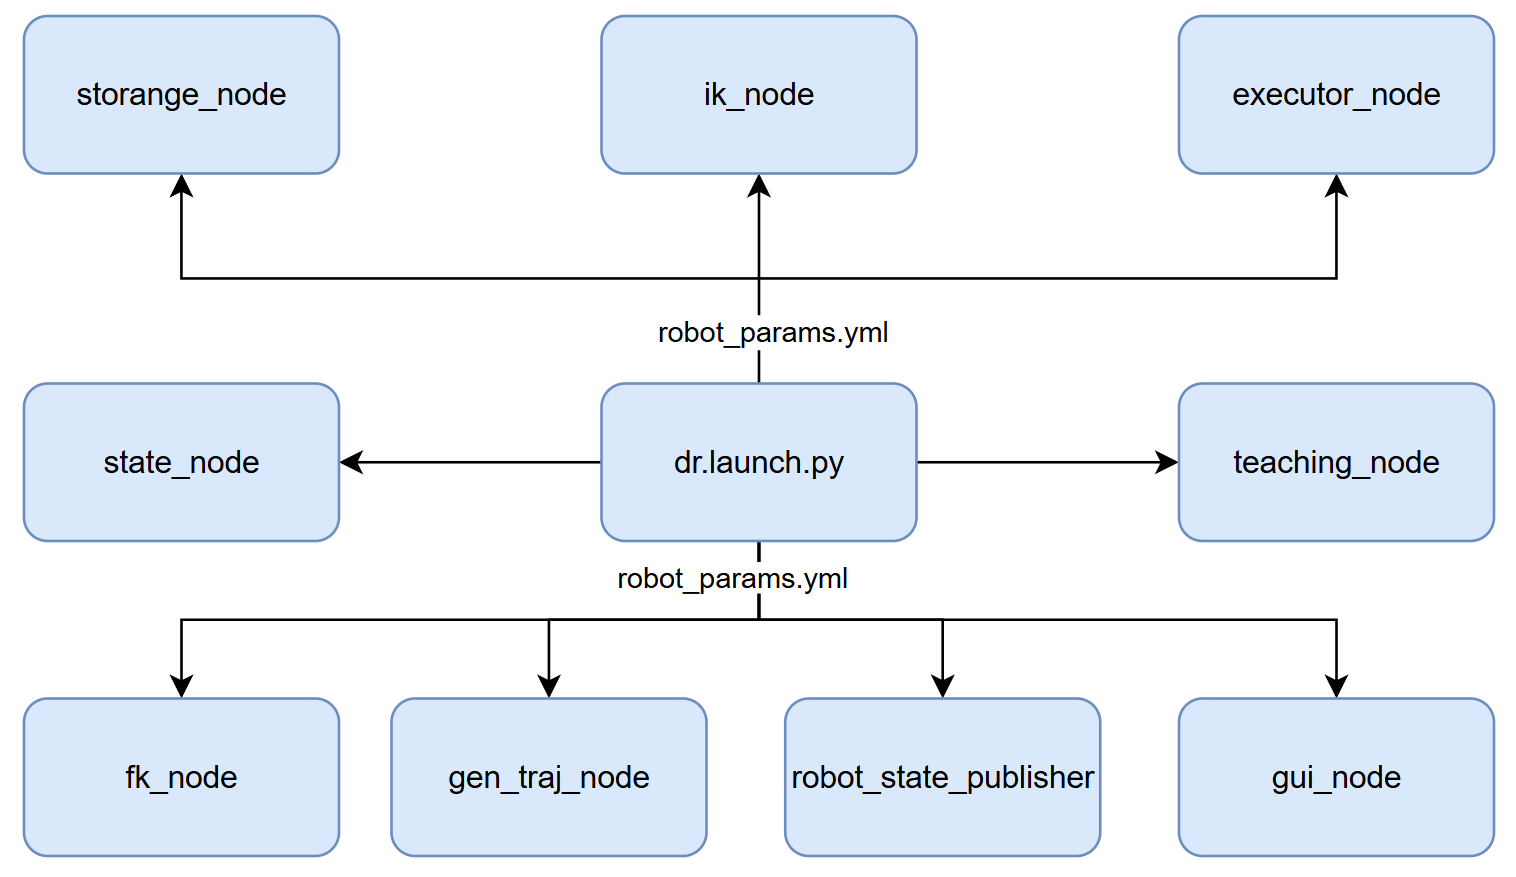
\includegraphics[width=0.85\linewidth]{ros2_arq_1.png}
    \caption{Esquema de levantamiento de nodos desde nodo launcher.}
    \label{fig:ros2_arq_1}
\end{figure}

A continuación se describe el propósito e interfaz principal de cada nodo. Los nodos de desarrollo propio se agrupan en paquetes con el prefijo \texttt{dr\_}; el nodo \texttt{robot\_state\_publisher} es el nodo estándar de ROS~2 que publica las transformaciones del árbol cinemático a partir del URDF y del tópico \texttt{/joint\_states}.

\begin{table}[H]
    \centering
    \caption{Nodos del sistema ROS~2 y sus interfaces principales.}
    \label{tab:ros2_nodos}
    \renewcommand{\arraystretch}{1.5}
    \begin{tabular}{l l p{7.5cm}}
        \toprule
        \textbf{Nodo} & \textbf{Paquete} & \textbf{Descripción e interfaz principal} \\
        \midrule

        \texttt{fk\_node} & \texttt{dr\_kinematics} &
            Resuelve la cinemática directa. Expone el servicio \texttt{/dr/solve\_fk}: recibe los ángulos articulares $\mathbf{q}$ y devuelve la pose cartesiana del efector final. \\

        \texttt{ik\_node} & \texttt{dr\_kinematics} &
            Resuelve la cinemática inversa analítica. Expone el servicio \texttt{/dr/solve\_ik}: recibe una pose cartesiana y devuelve el conjunto de soluciones articulares válidas. \\

        \texttt{gen\_traj\_node} & \texttt{dr\_trajectory} &
            Genera trayectorias en espacio articular o cartesiano con escalado de velocidades. Expone \texttt{/dr/gen\_traj}; consume internamente \texttt{/dr/solve\_ik} y \texttt{/dr/solve\_fk}. Se suscribe a \texttt{/dr/robot\_state} para obtener la configuración inicial. \\

        \texttt{state\_node} & \texttt{dr\_state} &
            Agrega el estado articular (\texttt{/dr/joint\_state}) y el estado de herramienta (\texttt{/dr/tool\_state}), calcula la pose cartesiana o configuración articular actual mediante cinemática directa o inversa según corresponda y publica el estado unificado del robot en \texttt{/dr/robot\_state}. \\

        \texttt{joint\_state\_bridge\_node} & \texttt{dr\_state} &
            Convierte \texttt{/dr/robot\_state} al mensaje estándar \texttt{sensor\_msgs\allowbreak/JointState} publicado en \texttt{/joint\_states}, necesario para la visualización en RViz y para el \texttt{robot\_state\_publisher}. \\

        \texttt{executor\_node} & \texttt{dr\_executor} &
            Ejecuta una trayectoria articular recibida como objetivo de la acción \texttt{/dr/execute}, publicando realimentación de posición en \texttt{/dr/joint\_state} a lo largo del recorrido. \\

        \texttt{storage\_node} & \texttt{dr\_storage} &
            Gestiona la persistencia de trayectorias en formato JSON. Expone los servicios \texttt{/dr/save\_traj}, \texttt{/dr/load\_traj}, \texttt{/dr/list\_trajs} y \texttt{/dr/delete\_traj}. \\

        \texttt{teaching\_node} & \texttt{dr\_teaching} &
            Convierte incrementos cartesianos recibidos en \texttt{/dr/\allowbreak teaching\_delta} en comandos de pose de herramienta publicados en \texttt{/dr/tool\_state}, habilitando el movimiento manual incremental del efector final. \\

        \texttt{gui\_node} & \texttt{dr\_gui} &
            Interfaz gráfica (PyQt5) que centraliza las funcionalidades del sistema: movimiento manual, enseñanza de puntos, generación y gestión de trayectorias, ejecución y análisis de variables cinemáticas. Se suscribe a \texttt{/dr/robot\_state}, publica en \texttt{/dr/teaching\_delta} y consume todos los servicios y la acción \texttt{/dr/execute}. \\

   \end{tabular}
\end{table}

% ======================================================================
\subsection{Interfaces personalizadas}
\label{sec:ros2_interfaces}

Todas las interfaces de comunicación fueron definidas de forma propia en el paquete \texttt{dr\_interfaces}. Se clasifican en mensajes, servicios y acciones.

En el caso de las trayectorias articulares, los mensajes de ROS~2 no admiten matrices bidimensionales de tamaño variable, por lo que se adoptó la convención de aplanarlas en vectores unidimensionales (\texttt{float64[]}). Cada grupo de seis valores consecutivos corresponde a una configuración articular $\mathbf{q} \in \mathbb{R}^6$, de modo que una trayectoria de $N$ puntos se representa como un vector de $6N$ elementos. El campo entero \texttt{points} acompaña siempre a \texttt{q\_traj} e indica el valor de $N$, necesario para reconstruir la matriz original al deserializar el mensaje.

\subsubsection*{Mensajes}

\begin{table}[H]
    \centering
    \caption{Mensajes personalizados (\texttt{dr\_interfaces/msg}).}
    \label{tab:ros2_msgs}
    \renewcommand{\arraystretch}{1.3}
    \begin{tabular}{l p{4.5cm} p{5.5cm}}
        \toprule
        \textbf{Mensaje} & \textbf{Campos} & \textbf{Descripción} \\
        \midrule
        \texttt{JointState} &
            \texttt{float64[6] q} \newline
            \texttt{float64[6] qd} \newline
            \texttt{float64[6] qdd} &
            Estado articular completo: posición, velocidad y aceleración de las seis articulaciones. \\

        \texttt{RobotState} &
            \texttt{float64[6] q} \newline
            \texttt{float64[6] qd} \newline
            \texttt{float64[6] qdd} \newline
            \texttt{float64[6] pose} &
            Estado unificado del robot: estado articular más pose cartesiana del efector final $(x,y,z,\alpha,\beta,\gamma)$. \\

        \texttt{ToolState} &
            \texttt{float64[6] pose} &
            Pose cartesiana de la herramienta $(x,y,z,\alpha,\beta,\gamma)$. Usada para comandar el movimiento del efector en modo \textit{teaching}. \\

        \texttt{TeachingDelta} &
            \texttt{float64 dx, dy, dz} \newline
            \texttt{float64 droll, dpitch, dyaw} &
            Incremento cartesiano solicitado desde la GUI para el movimiento manual del efector final. \\
        \bottomrule
    \end{tabular}
\end{table}

\subsubsection*{Servicios}

\begin{table}[H]
    \centering
    \caption{Servicios personalizados (\texttt{dr\_interfaces/srv}).}
    \label{tab:ros2_srvs}
    \renewcommand{\arraystretch}{1.3}
    \begin{tabular}{l p{3.8cm} p{3.8cm} p{2.8cm}}
        \toprule
        \textbf{Servicio} & \textbf{Request} & \textbf{Response} & \textbf{Descripción} \\
        \midrule
        \texttt{SolveFK} &
            \texttt{float64[6] q} &
            \texttt{float64[6] pose} \newline \texttt{bool success} &
            Cinemática directa. \\

        \texttt{SolveIK} &
            \texttt{float64[6] pose} \newline
            \texttt{float64[6] q0} \newline
            \texttt{bool force} &
            \texttt{float64[6] q} \newline \texttt{bool success} &
            Cinemática inversa analítica. \\

        \texttt{GenTraj} &
            \texttt{float64[] pose} \newline
            \texttt{int8 mode} \newline
            \texttt{int8 speed\_profile} &
            \texttt{float64[] q\_traj} \newline
            \texttt{int32 points} \newline
            \texttt{bool success} &
            Generación de trayectoria hacia una pose objetivo. \\

        \texttt{SaveTraj} &
            \texttt{string name} \newline
            \texttt{float64[] q\_traj} \newline
            \texttt{int32 points} &
            \texttt{bool success} &
            Persistencia de trayectoria en disco. \\

        \texttt{LoadTraj} &
            \texttt{string name} &
            \texttt{float64[] q\_traj} \newline
            \texttt{int32 points} \newline
            \texttt{bool success} &
            Carga de trayectoria desde disco. \\

        \texttt{ListTrajs} &
            --- &
            \texttt{string[] names} \newline
            \texttt{bool success} &
            Lista de trayectorias almacenadas. \\

        \texttt{DeleteTraj} &
            \texttt{string name} &
            \texttt{bool success} &
            Eliminación de trayectoria del disco. \\
        \bottomrule
    \end{tabular}
\end{table}

\subsubsection*{Acciones}

\begin{table}[H]
    \centering
    \caption{Acción personalizada (\texttt{dr\_interfaces/action}).}
    \label{tab:ros2_actions}
    \renewcommand{\arraystretch}{1.3}
    \begin{tabular}{l p{3.5cm} p{4cm} p{3.5cm}}
        \toprule
        \textbf{Acción} & \textbf{Goal} & \textbf{Feedback} & \textbf{Result} \\
        \midrule
        \texttt{Execute} &
            \texttt{float64[] q\_traj} \newline
            \texttt{int32 points} &
            \texttt{float64[6] q, qd, qdd} \newline
            \texttt{int32 point\_index} \newline
            \texttt{float64 progress} &
            \texttt{bool success} \newline
            \texttt{string message} \\
        \bottomrule
    \end{tabular}
\end{table}

% ======================================================================
\subsection{Interrelación entre nodos}
\label{sec:ros2_interrelacion}

Los nodos del sistema se interrelacionan a través de cuatro flujos funcionales que operan de forma concurrente. A continuación se describe cada uno.

\paragraph{Flujo de estado (permanente).}
El \texttt{state\_node} es el nodo central del sistema: agrega toda la información de posición del robot y la redistribuye de forma unificada. Recibe el estado articular desde \texttt{executor\_node} a través del tópico \texttt{/dr/joint\_state}, y los comandos de pose de herramienta desde \texttt{teaching\_node} a través de \texttt{/dr/tool\_state}. Con esta información, llama al servicio \texttt{/dr/solve\_fk} del \texttt{fk\_node} para calcular la pose cartesiana actual y publica el estado completo del robot en \texttt{/dr/robot\_state}. Este tópico es consumido por \texttt{gui\_node}, \texttt{teaching\_node} y \texttt{gen\_traj\_node}. Paralelamente, el \texttt{joint\_state\_bridge\_node} convierte \texttt{/dr/robot\_state} al formato estándar \texttt{sensor\_msgs/JointState} en \texttt{/joint\_states}, que es consumido por el \texttt{robot\_state\_publisher} para mantener el árbol de transformaciones TF y habilitar la visualización en RViz.

\paragraph{Flujo de movimiento manual (\textit{teaching}).}
Cuando el operador acciona los controles de movimiento manual en la GUI, el \texttt{gui\_node} publica un incremento cartesiano en \texttt{/dr/teaching\_delta}. El \texttt{teaching\_node} recibe este incremento y, a partir de la pose actual disponible en \texttt{/dr/robot\_state}, calcula la nueva pose objetivo y la publica en \texttt{/dr/tool\_state}. El \texttt{state\_node} recibe esta actualización, resuelve la cinemática inversa llamando a \texttt{/dr/solve\_ik} del \texttt{ik\_node} para obtener la configuración articular correspondiente, y publica el nuevo \texttt{/dr/robot\_state}, cerrando el ciclo de realimentación hacia la GUI.

\paragraph{Flujo de generación de trayectoria.}
Cuando el operador solicita generar una trayectoria desde la GUI, el \texttt{gui\_node} invoca el servicio \texttt{/dr/gen\_traj} del \texttt{gen\_traj\_node}. Este último consulta \texttt{/dr/robot\_state} para obtener la configuración articular inicial del robot, y luego llama iterativamente a \texttt{/dr/solve\_ik} del \texttt{ik\_node} y a \texttt{/dr/solve\_fk} del \texttt{fk\_node} para resolver las configuraciones articulares de cada punto vía y verificar la trayectoria generada. La trayectoria resultante, codificada como vector aplanado, es devuelta al \texttt{gui\_node} en la respuesta del servicio.

\paragraph{Flujo de ejecución de trayectoria.}
Una vez disponible la trayectoria, el \texttt{gui\_node} envía un objetivo (\textit{goal}) a la acción \texttt{/dr/execute} del \texttt{executor\_node}. Este recorre la trayectoria articular punto a punto, publicando en cada paso el estado articular actual en \texttt{/dr/joint\_state}. El \texttt{state\_node} procesa estos valores, actualiza \texttt{/dr/robot\_state} y lo publica, de modo que tanto la GUI como RViz reflejan el movimiento en tiempo real. Simultáneamente, el \texttt{executor\_node} envía realimentación al cliente de la acción con la posición articular actual, el índice del punto en curso y el progreso normalizado de la ejecución.

\paragraph{Flujo de gestión de trayectorias almacenadas.}
El \texttt{gui\_node} interactúa directamente con el \texttt{storage\_node} mediante los servicios \texttt{/dr/save\_traj}, \texttt{/dr/load\_traj}, \texttt{/dr/list\_trajs} y \texttt{/dr/delete\_traj} para persistir, recuperar y administrar trayectorias en disco. El \texttt{storage\_node} no tiene dependencias con ningún otro nodo del sistema, lo que garantiza su operación independiente.

% ======================================================================
\subsection{Modelo URDF}
\label{sec:ros2_urdf}

El modelo del robot se describe en formato URDF (\textit{Unified Robot Description Format}) y se aloja en el paquete \texttt{robot\_description}. Su estructura fue derivada directamente de la parametrización Denavit-Hartenberg definida en la sección~\ref{sec:modelado_cinematico}, garantizando consistencia geométrica entre ambas representaciones.

El árbol cinemático está compuesto por un eslabón raíz fijo (\texttt{world}), seis eslabones móviles (\texttt{link\_1} a \texttt{link\_6}) y un eslabón de herramienta (\texttt{tcp}), vinculados mediante seis articulaciones rotativas y una articulación fija. Cada articulación rotativa incorpora los parámetros de offset, traslación y rotación del eslabón correspondiente derivados de la tabla DH, de modo que la cadena cinemática resultante reproduce fielmente el modelo analítico. Las articulaciones 1 a 5 tienen límites de $\pm 2\pi$ rad ($\pm 360\degree$); la articulación 6 se declara de tipo \textit{continuous} en concordancia con el alcance libre definido en las especificaciones del robot.

El offset de herramienta ($T_{\text{tool}}$) se incorpora como una articulación fija entre \texttt{link\_6} y \texttt{tcp}, con una traslación de 0.190~m en el eje $Z$, valor consistente con el parámetro \texttt{T\_tool} de \texttt{robot\_params.yml}.

Cada eslabón incluye una geometría visual asociada a la malla STL correspondiente del modelo CAD desarrollado en \textit{Fusion 360} (sección~\ref{sec:CAD}). Los ejes de referencia de cada malla fueron alineados con los marcos DH durante el proceso de diseño, por lo que no fue necesario aplicar transformaciones adicionales entre el sistema de referencia cinemático y el visual.

Esto puede verse en la siguiente imagen correspondiente al entorno de simulación RViz2:

\begin{figure}[H]
    \centering
    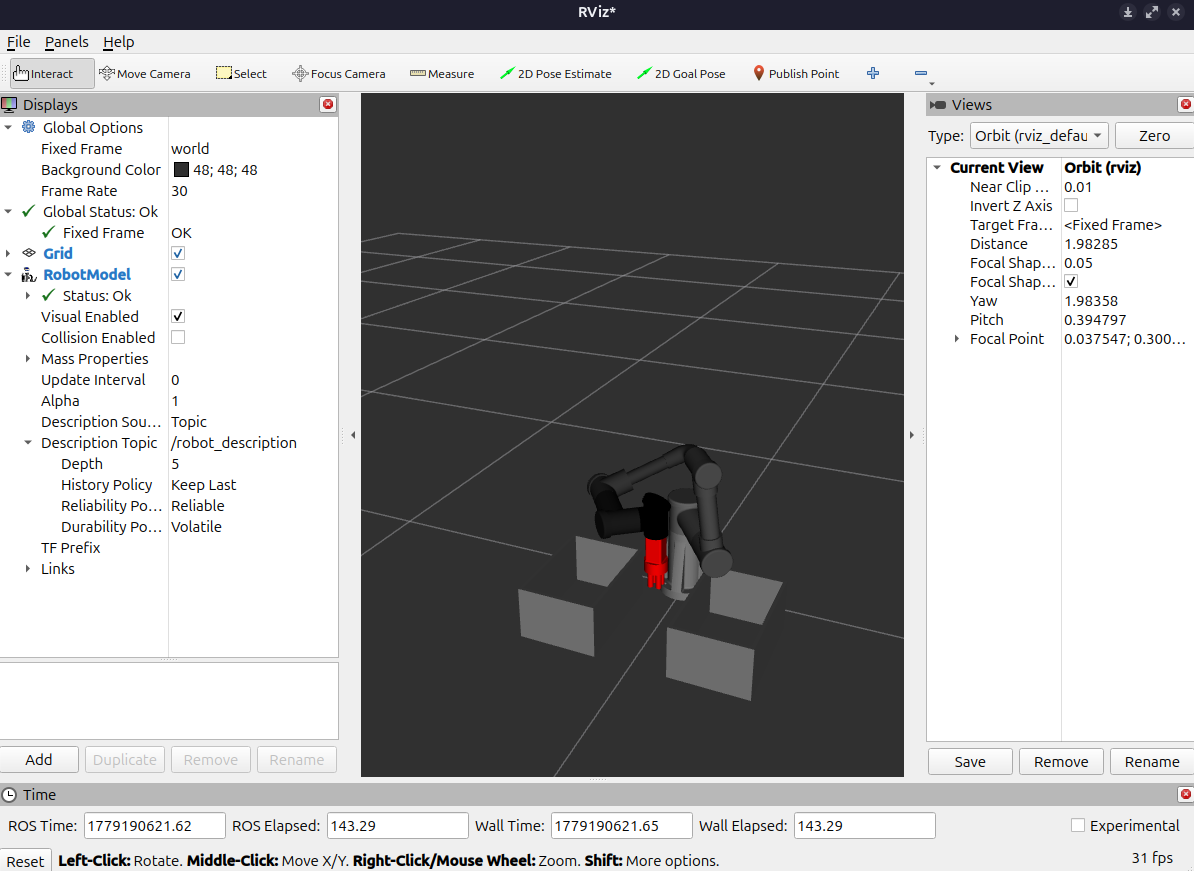
\includegraphics[width=0.85\linewidth]{rviz.png}
    \caption{Modelo URDF visualizado en simulaodr RViz2.}
    \label{fig:rviz}
\end{figure}

% ======================================================================
\subsection{Cinemática}
\label{sec:ros2_cinematica}

La cinemática directa e inversa se porta al entorno ROS~2 preservando los algoritmos analíticos desarrollados en la sección~\ref{sec:cinematica}. Sin embargo, la \textit{Robotics Toolbox} de Peter Corke, utilizada en MATLAB para operaciones de álgebra matricial homogénea y conversión de representaciones de orientación, no está disponible en el entorno Python de ROS~2.

Para resolver esta dependencia se implementó el módulo \colorbox{gray!20}{\texttt{transforms.py}}, alojado en el paquete \texttt{dr\_kinematics}. Este archivo replica las funciones del toolbox empleadas en el desarrollo, sin dependencias externas más allá de \texttt{numpy}:

\begin{itemize}
    \item \texttt{transl(x, y, z)}: matriz de transformación homogénea de traslación pura.
    \item \texttt{trotx($\theta$)}, \texttt{troty($\theta$)}, \texttt{trotz($\theta$)}: rotaciones elementales alrededor de los ejes $X$, $Y$ y $Z$.
    \item \texttt{inv\_T(T)}: inversa de una transformación homogénea, calculada eficientemente mediante $R^T$ y $-R^T\mathbf{p}$.
    \item \texttt{rot\_to\_rpy(R)}: extrae los ángulos de Euler ZYX (roll, pitch, yaw) desde una matriz de rotación, equivalente a \texttt{tr2rpy} del toolbox.
\end{itemize}

Los parámetros cinemáticos del robot (tabla DH, límites articulares, transformaciones de base y herramienta) se cargan en tiempo de ejecución desde \texttt{robot\_params.yml}, sin estar codificados en los nodos. Esto permite ajustar el modelo cinemático sin recompilar el código.

% ======================================================================
\subsection{Generación de trayectorias}
\label{sec:ros2_trayectorias}

El módulo de generación de trayectorias se porta al nodo \texttt{gen\_traj\_node}, preservando los dos modos de interpolación: espacio articular (modo 0) y espacio cartesiano (modo 1), y el mecanismo de escalado de velocidades y aceleraciones descrito en la sección~\ref{sec:escalamiento_velocidades}.

El servicio \texttt{/dr/gen\_traj} acepta \textbf{una única pose cartesiana objetivo} por solicitud, junto con el modo de interpolación y un perfil de velocidad (lento, medio o rápido). Al recibir la solicitud, el nodo obtiene la configuración articular actual desde \texttt{/dr/robot\_state} y genera la trayectoria desde esa configuración hasta el punto objetivo.

Esta decisión de diseño introduce una \textbf{limitación respecto a la implementación en MATLAB}: en \texttt{gen\_traj.m}, la función recibía la lista completa de puntos vía y generaba una única trayectoria continua a través de todos ellos, aprovechando la capacidad de \texttt{mstraj} de interpolar sin detención en los puntos intermedios. En ROS~2, dado que el servicio acepta un solo punto por solicitud, cada llamada genera una trayectoria independiente con velocidad inicial y final nula. Como consecuencia, \textbf{el robot se detiene completamente en cada punto vía} antes de recibir la siguiente solicitud, lo que impide la interpolación fluida entre segmentos consecutivos.

Esta limitación podría resolverse en el futuro rediseñando el servicio para aceptar una lista de puntos vía en una única solicitud, replicando el comportamiento de \texttt{mstraj} en el entorno ROS~2.

% ======================================================================
\subsection{Teaching}
\label{sec:ros2_teaching}

El modo \textit{teaching} permite desplazar el efector final de forma incremental desde la interfaz gráfica, capturando configuraciones intermedias que luego se encadenan para construir una trayectoria. El mecanismo se divide en dos componentes: el nodo de \textit{teaching} y la pestaña dedicada en la interfaz gráfica.

\subsubsection*{Nodo de teaching}

El \texttt{teaching\_node} actúa como un convertidor de desplazamientos relativos a poses absolutas. Al iniciarse, se suscribe a \texttt{/dr/robot\_state} para obtener y actualizar continuamente la configuración articular actual $\mathbf{q}_0$ y la pose cartesiana correspondiente $\mathbf{c}_0 = [x,\,y,\,z,\,r,\,p,\,y]^\top$.

Cuando la interfaz gráfica publica un incremento en \texttt{/dr/teaching\_delta} --- mensaje \texttt{TeachingDelta} con campos \texttt{dx, dy, dz, droll, dpitch, dyaw} --- el nodo suma dicho incremento a $\mathbf{c}_0$ y publica la pose absoluta resultante en \texttt{/dr/tool\_state}:
\[
\mathbf{c}_{\text{objetivo}} = \mathbf{c}_0 + \Delta\mathbf{c}
\]
Este enfoque garantiza que cada desplazamiento sea relativo a la pose \textit{actual} del robot, independientemente de si el robot se ha movido entre pulsos de botón.

\subsubsection*{Pestaña de teaching en la GUI}

La pestaña \textit{Teaching} de la interfaz gráfica centraliza el flujo de trabajo de enseñanza de puntos. Su estructura es la siguiente:

\begin{itemize}
    \item \textbf{Tabla de estado actual.} Muestra en tiempo real la configuración articular $\mathbf{q}$ (en radianes) y la pose cartesiana $[x,y,z,\text{roll},\text{pitch},\text{yaw}]$ del efector final. Los valores se actualizan cada vez que el nodo recibe un mensaje en \texttt{/dr/robot\_state}.

    \item \textbf{Controles de jog.} Para cada uno de los seis grados de libertad cartesianos (X, Y, Z, Roll, Pitch, Yaw) se dispone de un par de botones \texttt{+} y \texttt{--}. Al presionar cualquiera de ellos, la función \texttt{send\_delta(axis, sign)} construye un mensaje \texttt{TeachingDelta} con el incremento correspondiente al eje seleccionado y lo publica en \texttt{/dr/teaching\_delta}. El nodo de \textit{teaching} procesa el delta y publica la nueva pose objetivo en \texttt{/dr/tool\_state}, que a su vez el nodo de cinemática inversa resuelve y envía al estado del robot.

    \item \textbf{Paso de jog (\textit{step}).} Un \textit{spinbox} configurable entre $0{,}001$ y $0{,}1$\,m/rad determina el módulo del incremento aplicado en cada pulsación. Este valor se utiliza directamente en \texttt{send\_delta}.

    \item \textbf{Modo de interpolación y velocidad.} Un combo de modo (\textit{Articular} / \textit{Cartesiano}) y un combo de velocidad (\textit{Lento} / \textit{Medio} / \textit{Rápido}) acompañan cada waypoint capturado, de modo que la trayectoria resultante puede combinar segmentos con diferentes parámetros.

    \item \textbf{Captura de posición.} El botón \textit{``Capturar posición''} lee la pose actual de la tabla de estado y la almacena en la lista interna de waypoints junto con el modo y la velocidad seleccionados en ese instante.

    \item \textbf{Gestión de waypoints.} El botón \textit{``Ver lista de waypoints''} abre un diálogo (\texttt{WaypointDialog}) que muestra todos los puntos capturados. Desde este diálogo el usuario puede eliminar puntos individuales antes de confirmar la trayectoria.

    \item \textbf{Finalización.} El campo de texto de nombre y el botón \textit{``Finalizar''} desencadenan el proceso de generación completo: se itera sobre la lista de waypoints llamando al servicio \texttt{/dr/gen\_traj} para cada par de puntos consecutivos, las trayectorias parciales se concatenan y el resultado se persiste en disco llamando al servicio \texttt{/dr/save\_traj}.
\end{itemize}

% ======================================================================
\subsection{Interfaz gráfica}
\label{sec:ros2_gui}

La interfaz gráfica fue desarrollada con \textit{PyQt5} e integra en un único proceso tanto la lógica de comunicación con ROS~2 como la presentación visual. Para mantener la responsividad de la interfaz, el \textit{spin} de ROS~2 se ejecuta en un hilo demonio (\texttt{threading.Thread}), mientras que todas las actualizaciones de widgets se realizan mediante señales Qt (\texttt{pyqtSignal}), evitando accesos al hilo principal desde el hilo de ROS~2. Las llamadas a servicios, que son bloqueantes, se realizan también en hilos separados sincronizados mediante \texttt{threading.Event}.

La ventana principal (\texttt{MainWindow}) se organiza en dos pestañas: \textit{Teaching} (descrita en la sección~\ref{sec:ros2_teaching}) y \textit{Ejecutar}.

\subsubsection*{Pestaña de ejecución}

La pestaña \textit{Ejecutar} permite cargar, recorrer y analizar trayectorias almacenadas. Sus componentes principales son:

\begin{itemize}
    \item \textbf{Tabla de estado actual.} Idéntica a la de la pestaña \textit{Teaching}: muestra $\mathbf{q}$ y la pose cartesiana en tiempo real.

    \item \textbf{Tabla de trayectorias disponibles.} Cada fila corresponde a una trayectoria almacenada e incluye columnas de nombre, fecha de creación, número de puntos y dos acciones:
        \begin{itemize}
            \item \textit{Recorrer}: carga la trayectoria llamando a \texttt{/dr/load\_traj} y envía una solicitud a la acción \texttt{/dr/execute}. Durante la ejecución, la pestaña \textit{Teaching} se deshabilita para evitar conflictos.
            \item \textit{Eliminar}: solicita confirmación al usuario y, de confirmarse, llama a \texttt{/dr/delete\_traj} y refresca la tabla.
            \item \textit{Analizar}: habilitado únicamente tras ejecutar la trayectoria correspondiente. Abre el diálogo de análisis descrito a continuación.
        \end{itemize}

    \item \textbf{Barra de progreso y etiqueta de estado.} Se actualizan en tiempo real a partir de los mensajes de \textit{feedback} de la acción \texttt{/dr/execute}, que reportan el índice del punto en curso. Al completarse la acción, la etiqueta refleja el resultado (\textit{éxito} o \textit{error}).
\end{itemize}

A continuación, se presentan imágenes correspondientes a cada pestaña.

\begin{figure}[H]
    \centering
    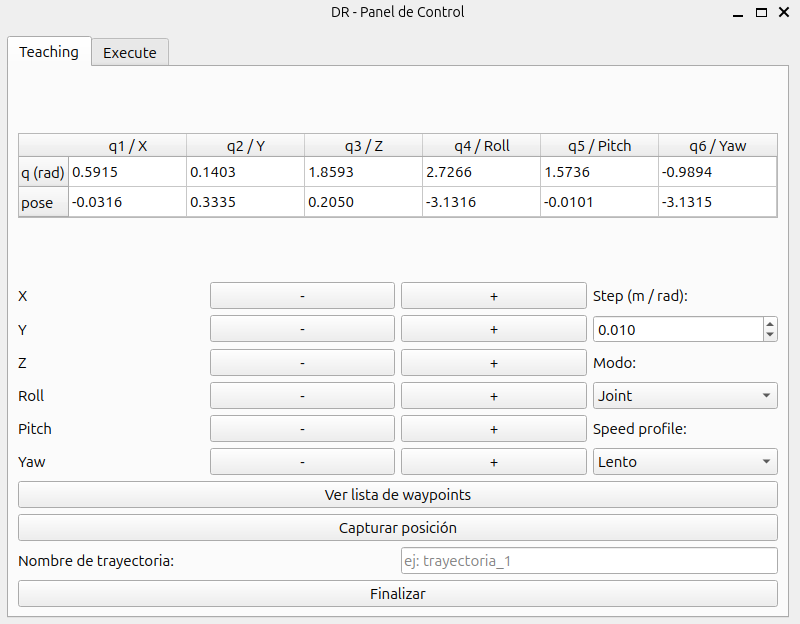
\includegraphics[width=0.85\linewidth]{gui_1.png}
    \caption{Interfáz gráfica de usuario en ROS 2 - Pestaña de teaching.}
    \label{fig:gui_1}
\end{figure}

\begin{figure}[H]
    \centering
    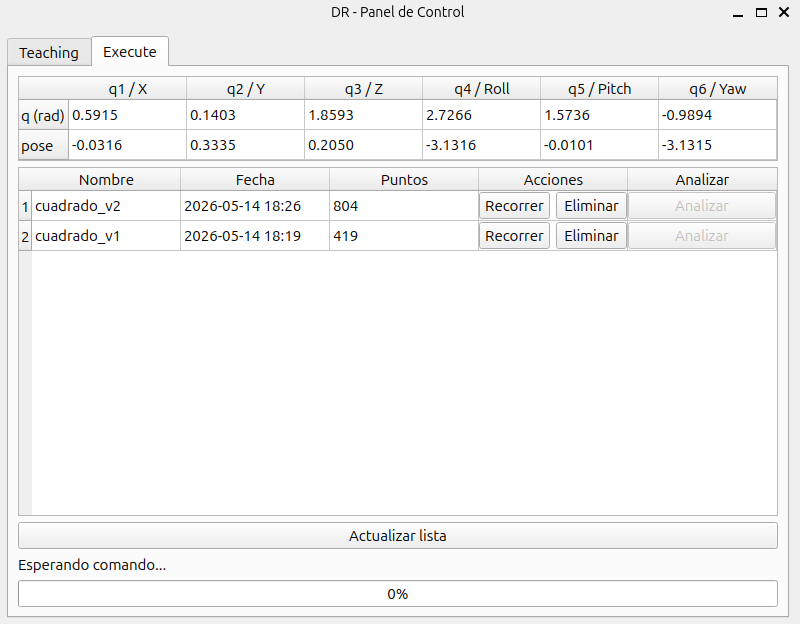
\includegraphics[width=0.85\linewidth]{gui_2.png}
    \caption{Interfáz gráfica de usuario en ROS 2 - Pestaña de ejecución.}
    \label{fig:gui_2}
\end{figure}

\subsubsection*{Diálogo de análisis}

Al finalizar la ejecución de una trayectoria, el botón \textit{Analizar} abre el \texttt{AnalysisDialog}, un diálogo con cuatro pestañas de visualización:

\begin{enumerate}
    \item \textbf{Coordenadas articulares}: evolución temporal de $q_1, \ldots, q_6$ junto con los límites articulares $\pm q_{\max}$ y el perfil de velocidades y aceleraciones articulares con sus respectivos límites.
    \item \textbf{Posición cartesiana del EF}: evolución de $x, y, z$ y los ángulos de Euler (roll, pitch, yaw) computados mediante cinemática directa.
    \item \textbf{Velocidad y aceleración lineal}: norma de la velocidad y aceleración lineales del efector final, calculadas a través del Jacobiano geométrico, con comparativa frente a los límites $v_{\max}$ y $a_{\max}$.
    \item \textbf{Velocidad y aceleración angular}: norma de la velocidad y aceleración angulares del efector final, con comparativa frente a $\omega_{\max}$ y $\alpha_{\max}$.
\end{enumerate}

El cálculo de cinemática directa para todas las muestras de la trayectoria se realiza en un hilo de fondo antes de renderizar los gráficos, de modo que la interfaz no se bloquea durante el proceso. Los gráficos se incrustan directamente en las pestañas del diálogo mediante \texttt{FigureCanvas} de \textit{Matplotlib}, sin abrir ventanas externas.

La siguientes imágenes muestran las 4 pestañas de análisis:

\begin{figure}[H]
    \centering
    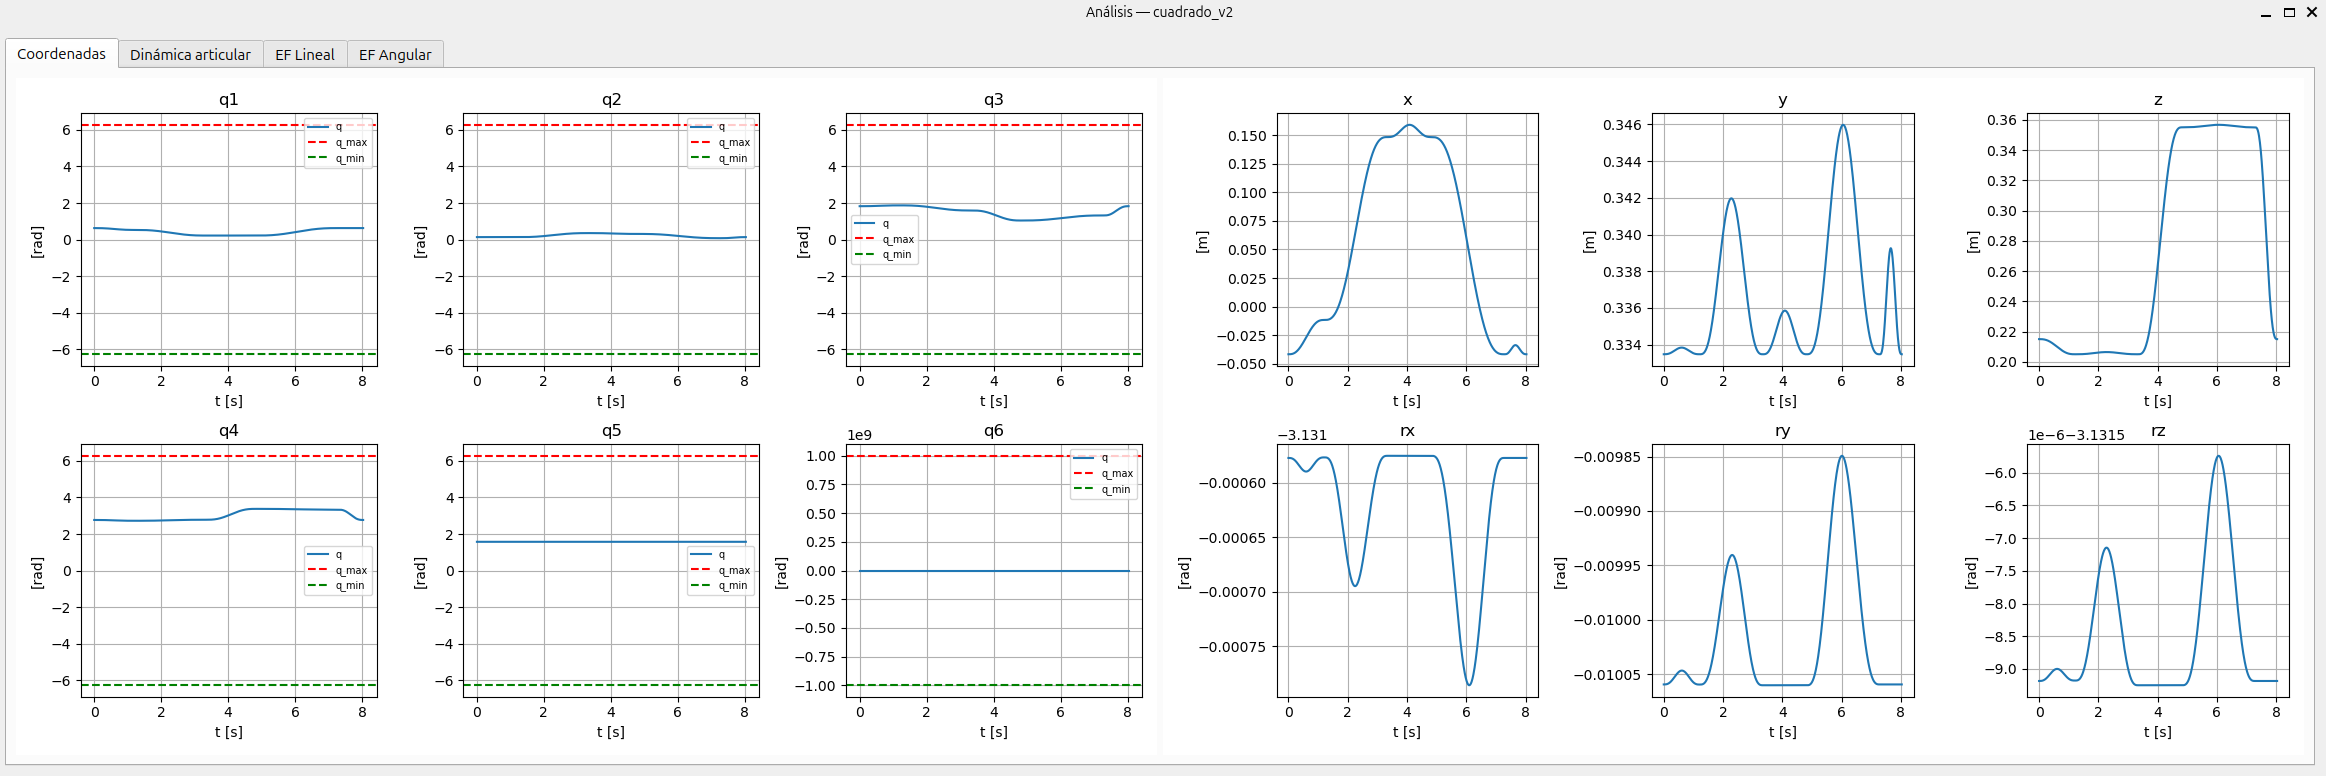
\includegraphics[width=1\linewidth]{gui_analisis_1.png}
    \caption{Interfáz gráfica de usuario - Pestaña de análisis: evolución de coordenadas cartesianas del efector final y coordenadas articulares de articulaciones.}
    \label{fig:gui_analisis_1}
\end{figure}

\begin{figure}[H]
    \centering
    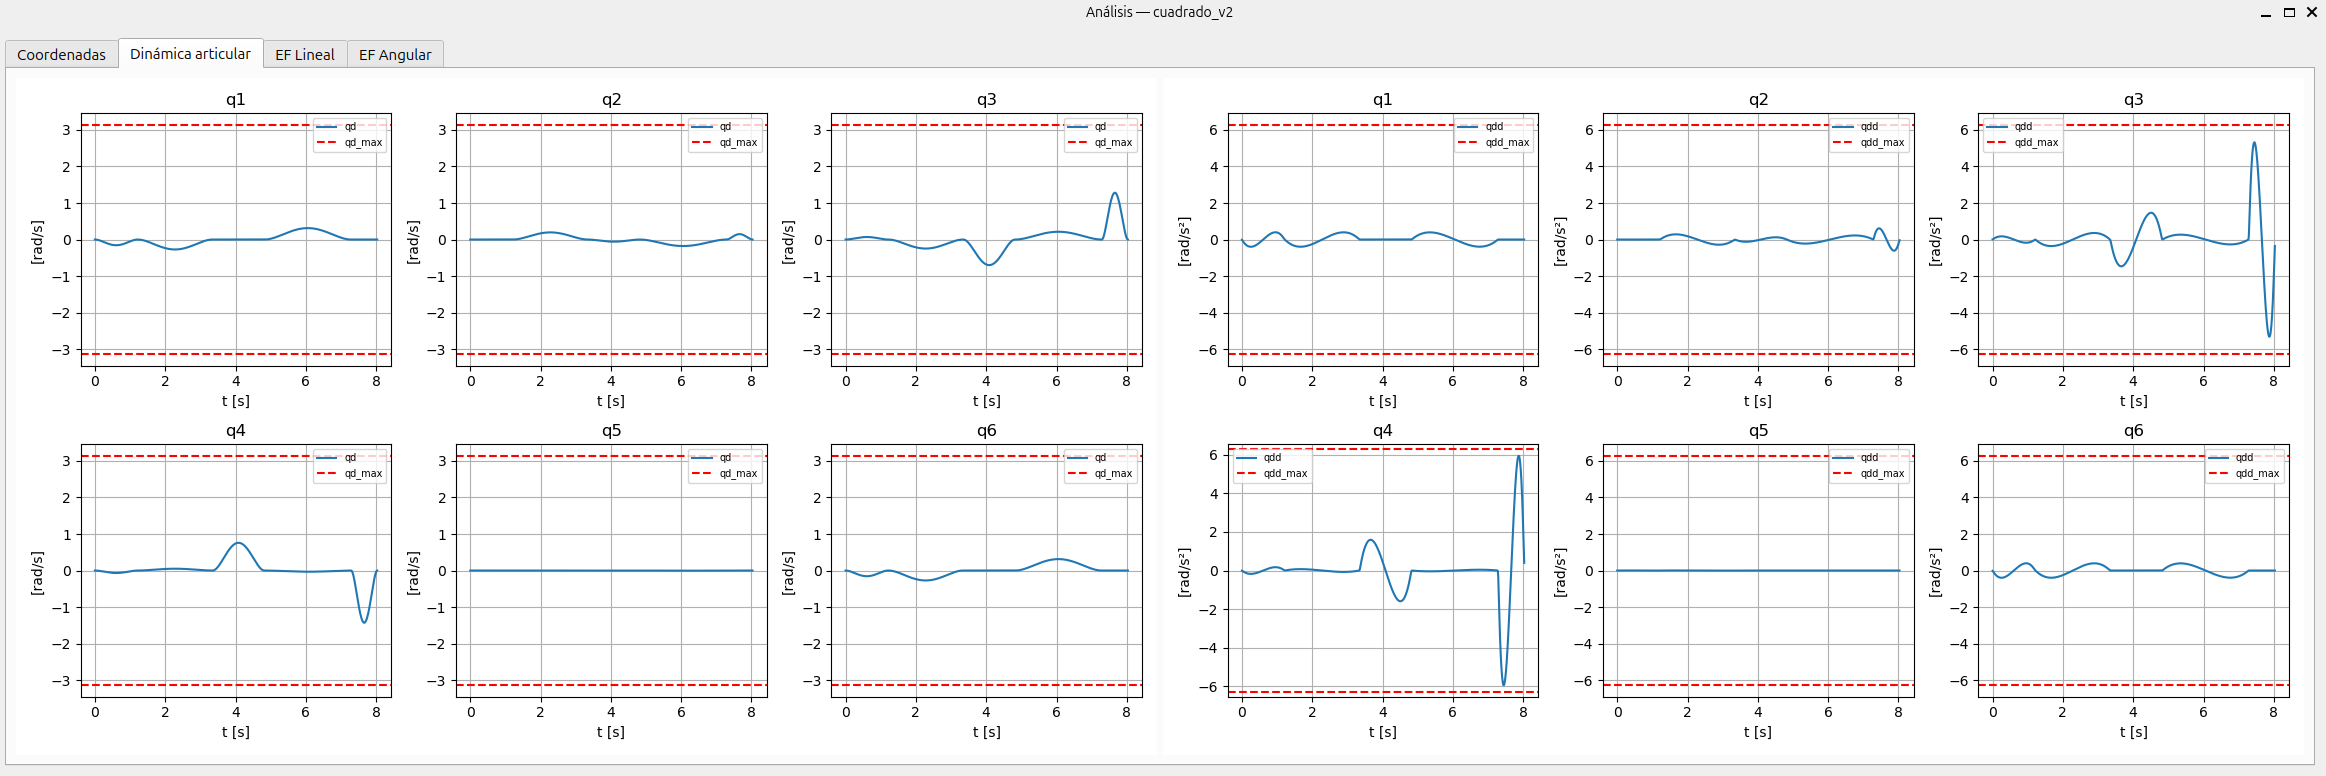
\includegraphics[width=1\linewidth]{gui_analisis_2.png}
    \caption{Interfáz gráfica de usuario - Pestaña de análisis: evolución de de velocidad articular y aceleración articular.}
    \label{fig:gui_analisis_2}
\end{figure}

\begin{figure}[H]
    \centering
    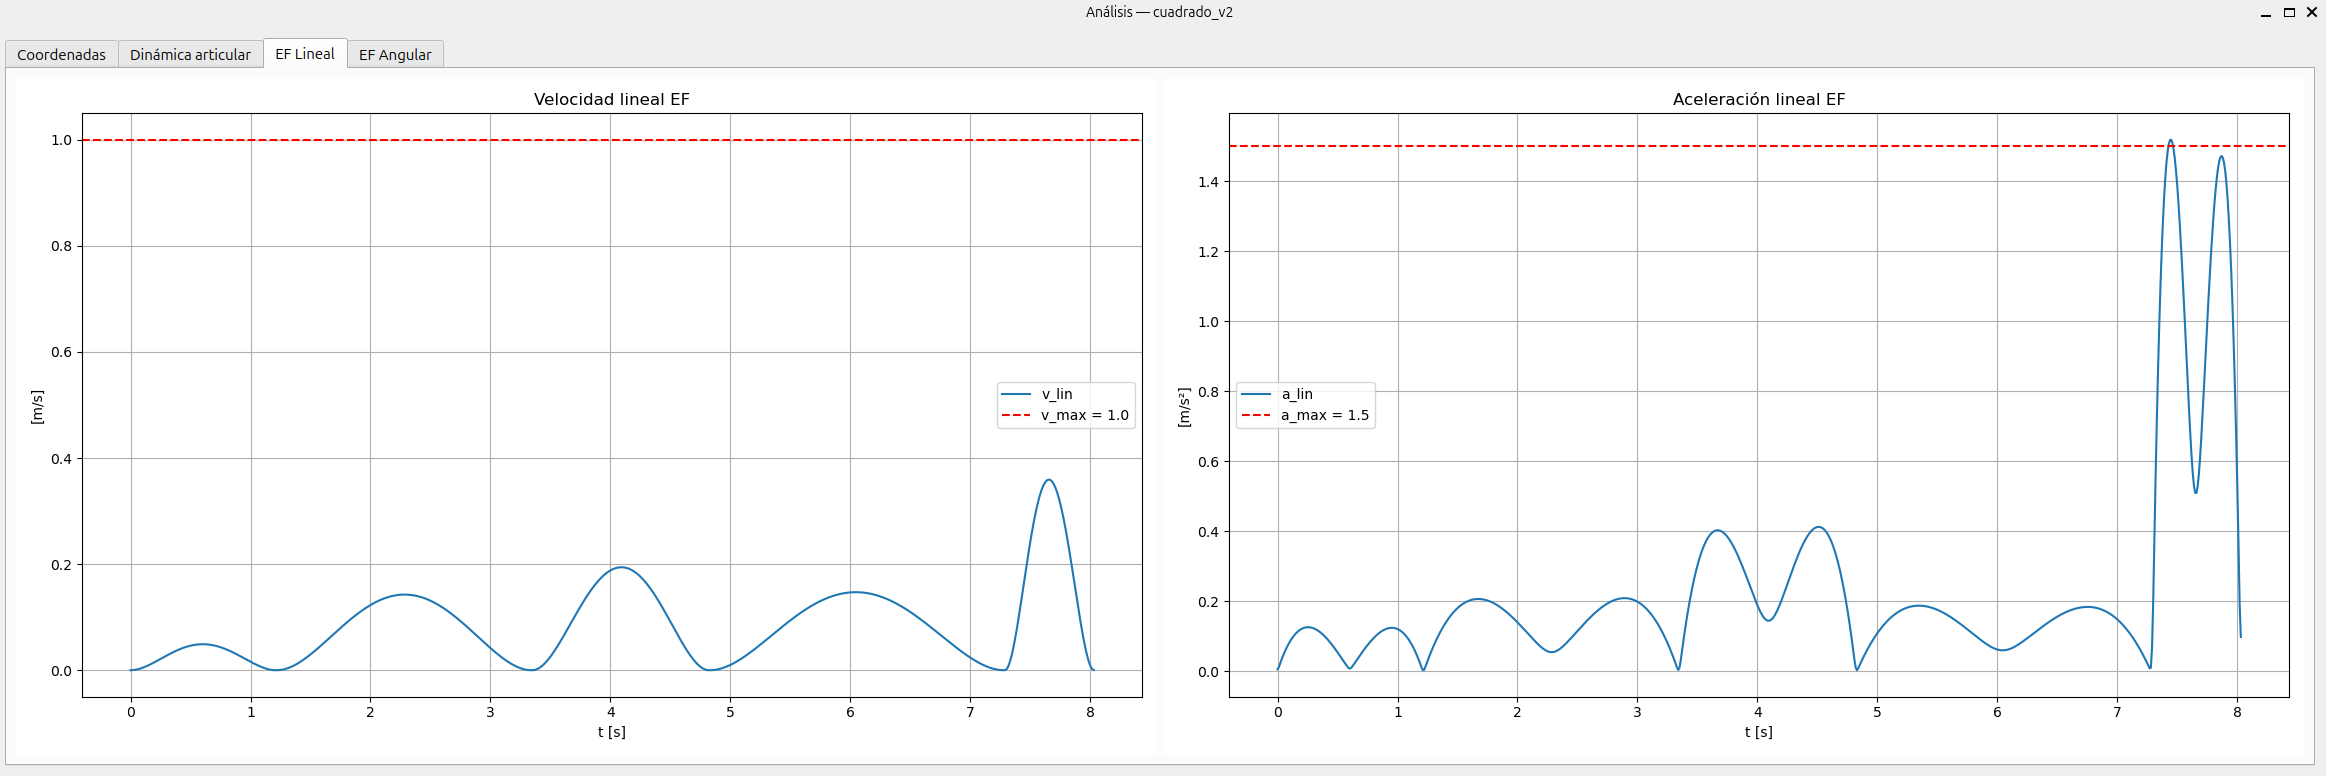
\includegraphics[width=1\linewidth]{gui_analisis_3.png}
    \caption{Interfáz gráfica de usuario - Pestaña de análisis: evolución de velocidad lineal y angular del efector final.}
    \label{fig:gui_analisis_3}
\end{figure}

\begin{figure}[H]
    \centering
    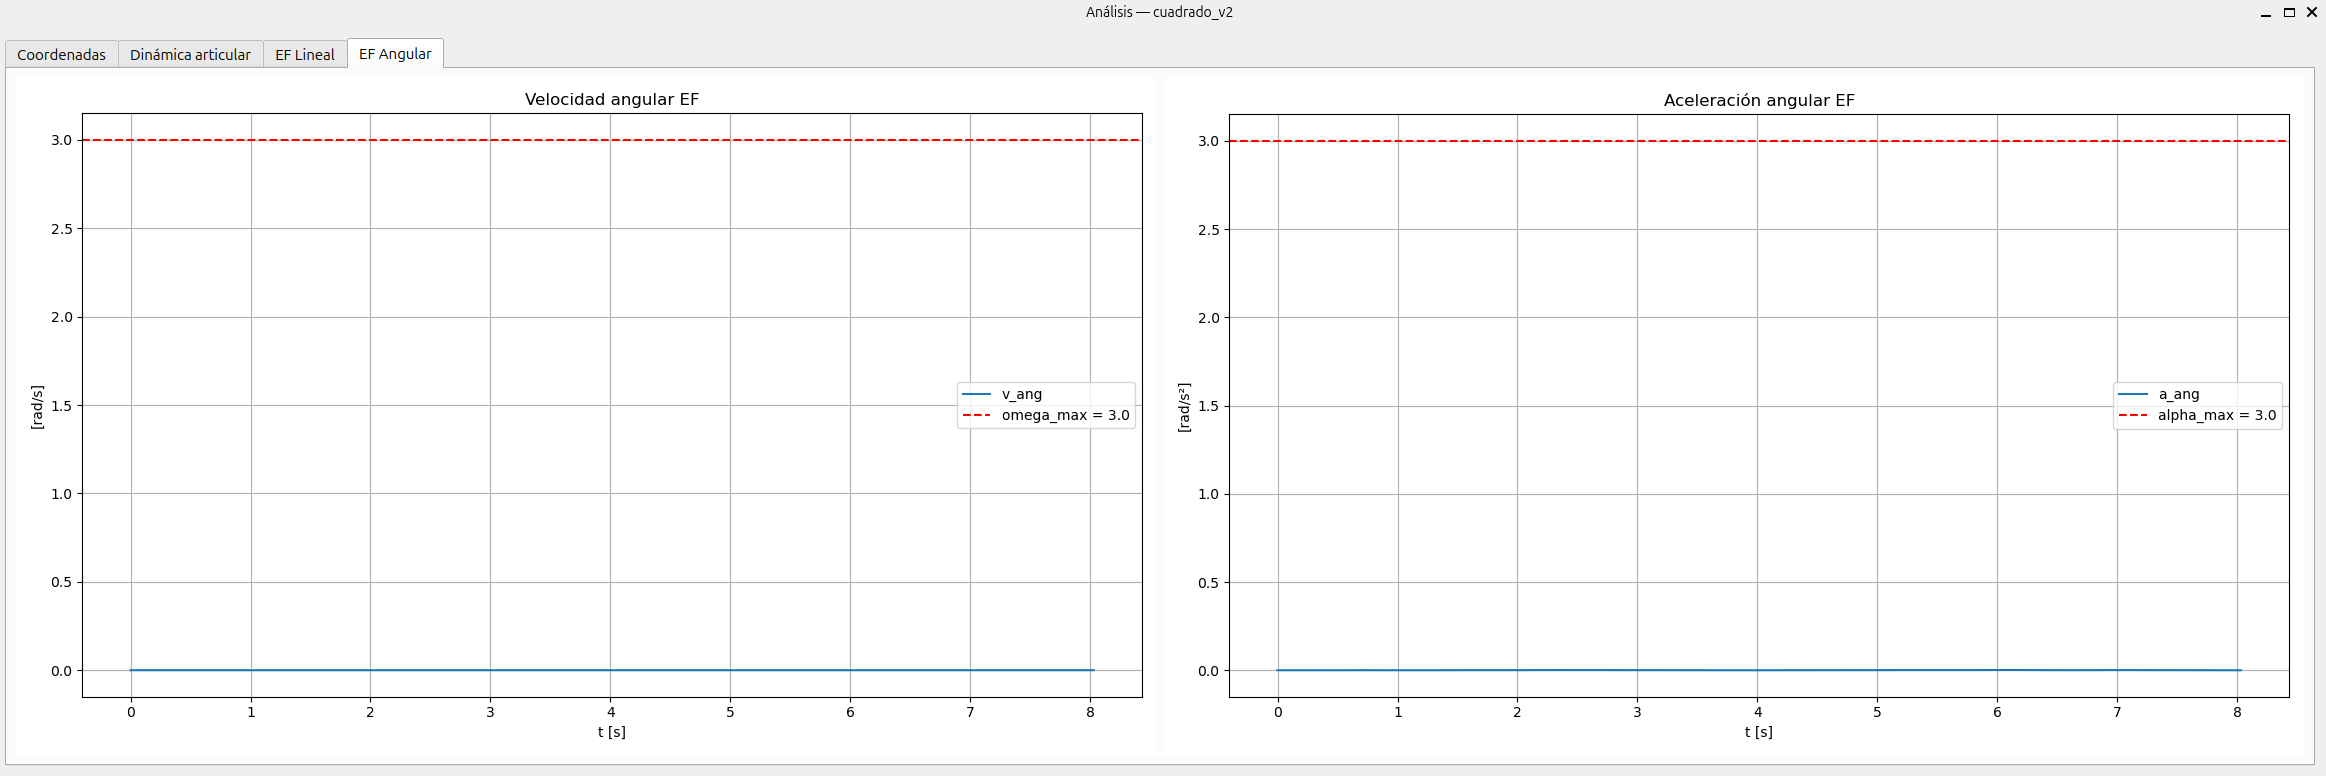
\includegraphics[width=1\linewidth]{gui_analisis_4.png}
    \caption{Interfáz gráfica de usuario - Pestaña de análisis: evolulución de aceleración lineal y angular del efector final.}    
    \label{fig:gui_analisis_4}
\end{figure}

De la misma manera al análisis en MATLAB, se presentan los valores obtenido en conjunto con sus máximos definidos para poder verificar el funcionamiento.

% ======================================================================
\newpage
\section{Verificación de productividad en entorno ROS~2}
\label{sec:verificacion_productividad}

Con el objetivo de evaluar el desempeño del sistema desarrollado, se busca verificar que el robot sea capaz de cumplir con el objetivo de productividad establecido: 300 transferencias por hora, lo que equivale a un período de ciclo de 12 segundos por transferencia. Para ello, se utiliza el sistema de \textit{teaching} implementado en ROS~2 para describir la trayectoria completa de la tarea, ejecutarla en el entorno de simulación y analizar las variables cinemáticas resultantes.

%
% ============
%
\subsection{Etapa 1: \textit{Teaching} de la trayectoria}
\label{sec:verif_teaching}

Utilizando la interfaz de \textit{teaching} implementada con PyQt5, se capturan los nueve puntos vía que describen un ciclo completo de la tarea del robot. La figura~\ref{fig:verif_posturas} muestra las nueve posturas del manipulador correspondientes a cada punto capturado.

\begin{figure}[H]
    \centering
    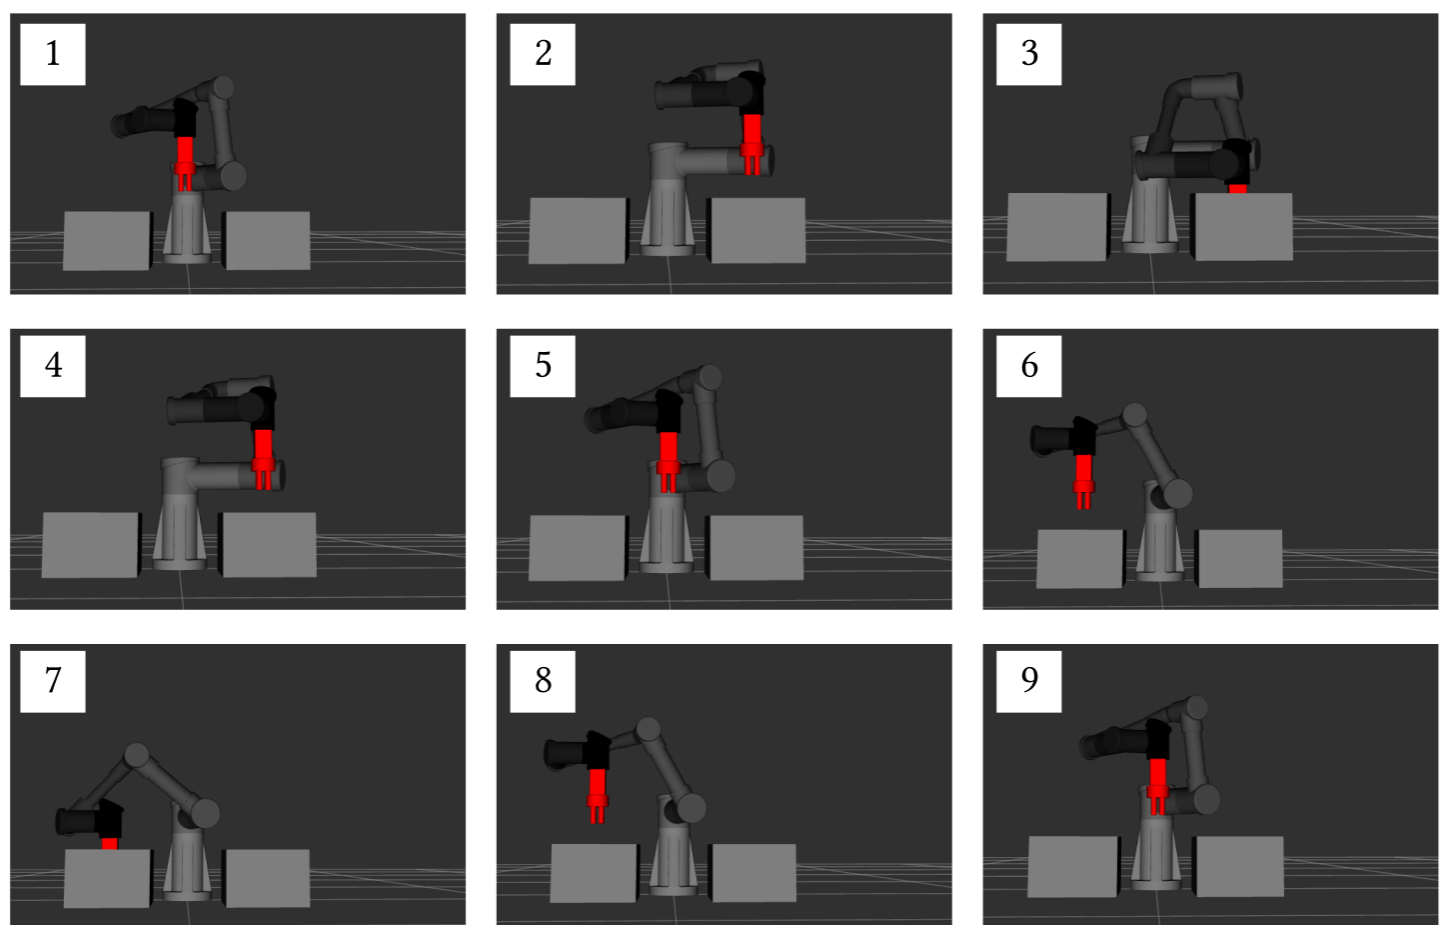
\includegraphics[width=0.85\linewidth]{verif_posturas.png}
    \caption{Nueve posturas del robot correspondientes a un ciclo completo de la tarea.}
    \label{fig:verif_posturas}
\end{figure}

Los puntos vía capturados describen el ciclo de la siguiente manera:

\begin{enumerate}
    \item \textbf{Postura de punto medio} --- configuración inicial del ciclo, utilizada como postura de espera segura y alejada de los límites articulares.
    \item \textbf{Postura sobre caja de \textit{picking}} --- el efector final se posiciona por encima de la caja de origen, previo al descenso.
    \item \textbf{Postura dentro de caja de \textit{picking}} --- el efector desciende al interior de la caja de origen para realizar la toma del objeto.
    \item \textbf{Postura sobre caja de \textit{picking}} --- el efector retorna a la posición elevada sobre la caja de origen con el objeto tomado.
    \item \textbf{Postura de punto medio (intermedia)} --- el robot transita por el punto medio para garantizar una trayectoria libre de interferencias entre origen y destino.
    \item \textbf{Postura sobre caja de \textit{placement}} --- el efector se posiciona por encima de la caja de destino, previo al descenso.
    \item \textbf{Postura dentro de caja de \textit{placement}} --- el efector desciende al interior de la caja de destino para depositar el objeto.
    \item \textbf{Postura sobre caja de \textit{placement}} --- el efector retorna a la posición elevada sobre la caja de destino.
    \item \textbf{Postura de punto medio (final)} --- el robot regresa a la postura de espera, completando el ciclo.
\end{enumerate}

La figura~\ref{fig:verif_waypoints} muestra la lista de puntos vía cartesianos registrados en la interfaz, con su posición, modo de interpolación y perfil de velocidad de llegada.

\begin{figure}[H]
    \centering
    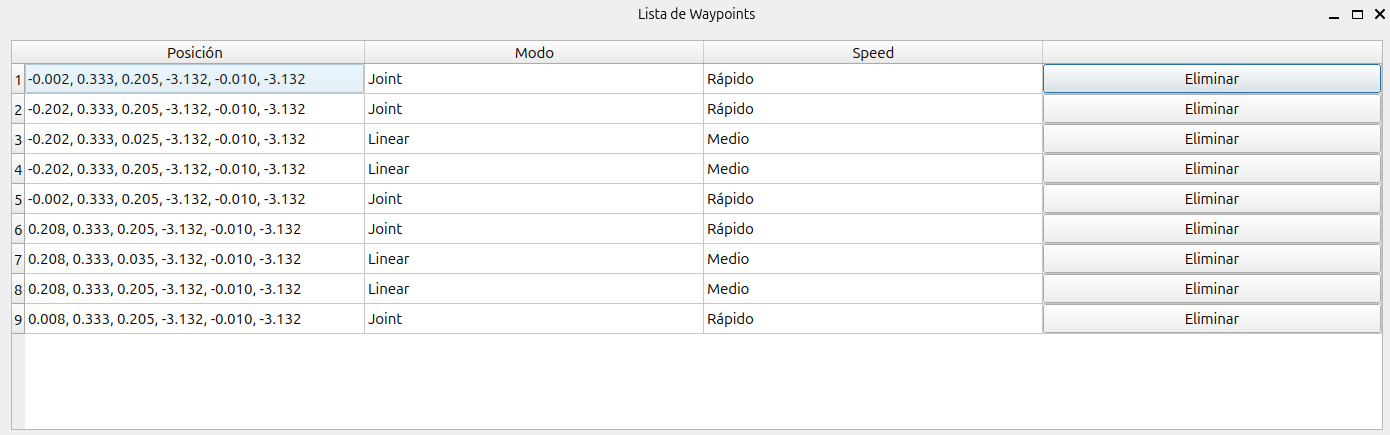
\includegraphics[width=0.85\linewidth]{verif_waypoints.png}
    \caption{Lista de puntos vía cartesianos capturados mediante \textit{teaching}, con modo de interpolación y velocidad de llegada.}
    \label{fig:verif_waypoints}
\end{figure}

%
% ============
%
\subsection{Etapa 2: Recorrido de la trayectoria}
\label{sec:verif_ejecucion}

Desde la pestaña \textit{Ejecutar} de la interfaz gráfica implementada en PyQt5, se selecciona la trayectoria generada en la etapa anterior para cargar sus posiciones y ejecutar el recorrido. De forma simultánea, se valida visualmente la correcta definición de la trayectoria en el entorno de simulación RViz2, verificando que el manipulador recorra las posturas definidas en el orden y con las características de interpolación establecidas durante el \textit{teaching}.

%
% ============
%
\subsection{Etapa 3: Análisis cinemático}
\label{sec:verif_analisis}

Una vez finalizada la ejecución, se accede al análisis cinemático completo desde la opción \textit{Analizar} disponible en la pestaña \textit{Ejecutar} de la interfaz gráfica. El diálogo de análisis presenta cuatro pestañas con la evolución temporal de las variables cinemáticas del manipulador a lo largo del ciclo ejecutado.

La figura~\ref{fig:verif_an1} muestra la evolución de las coordenadas articulares $q_1$ a $q_6$ y de la posición cartesiana del efector final $(x, y, z, \text{roll}, \text{pitch}, \text{yaw})$.

\begin{figure}[H]
    \centering
    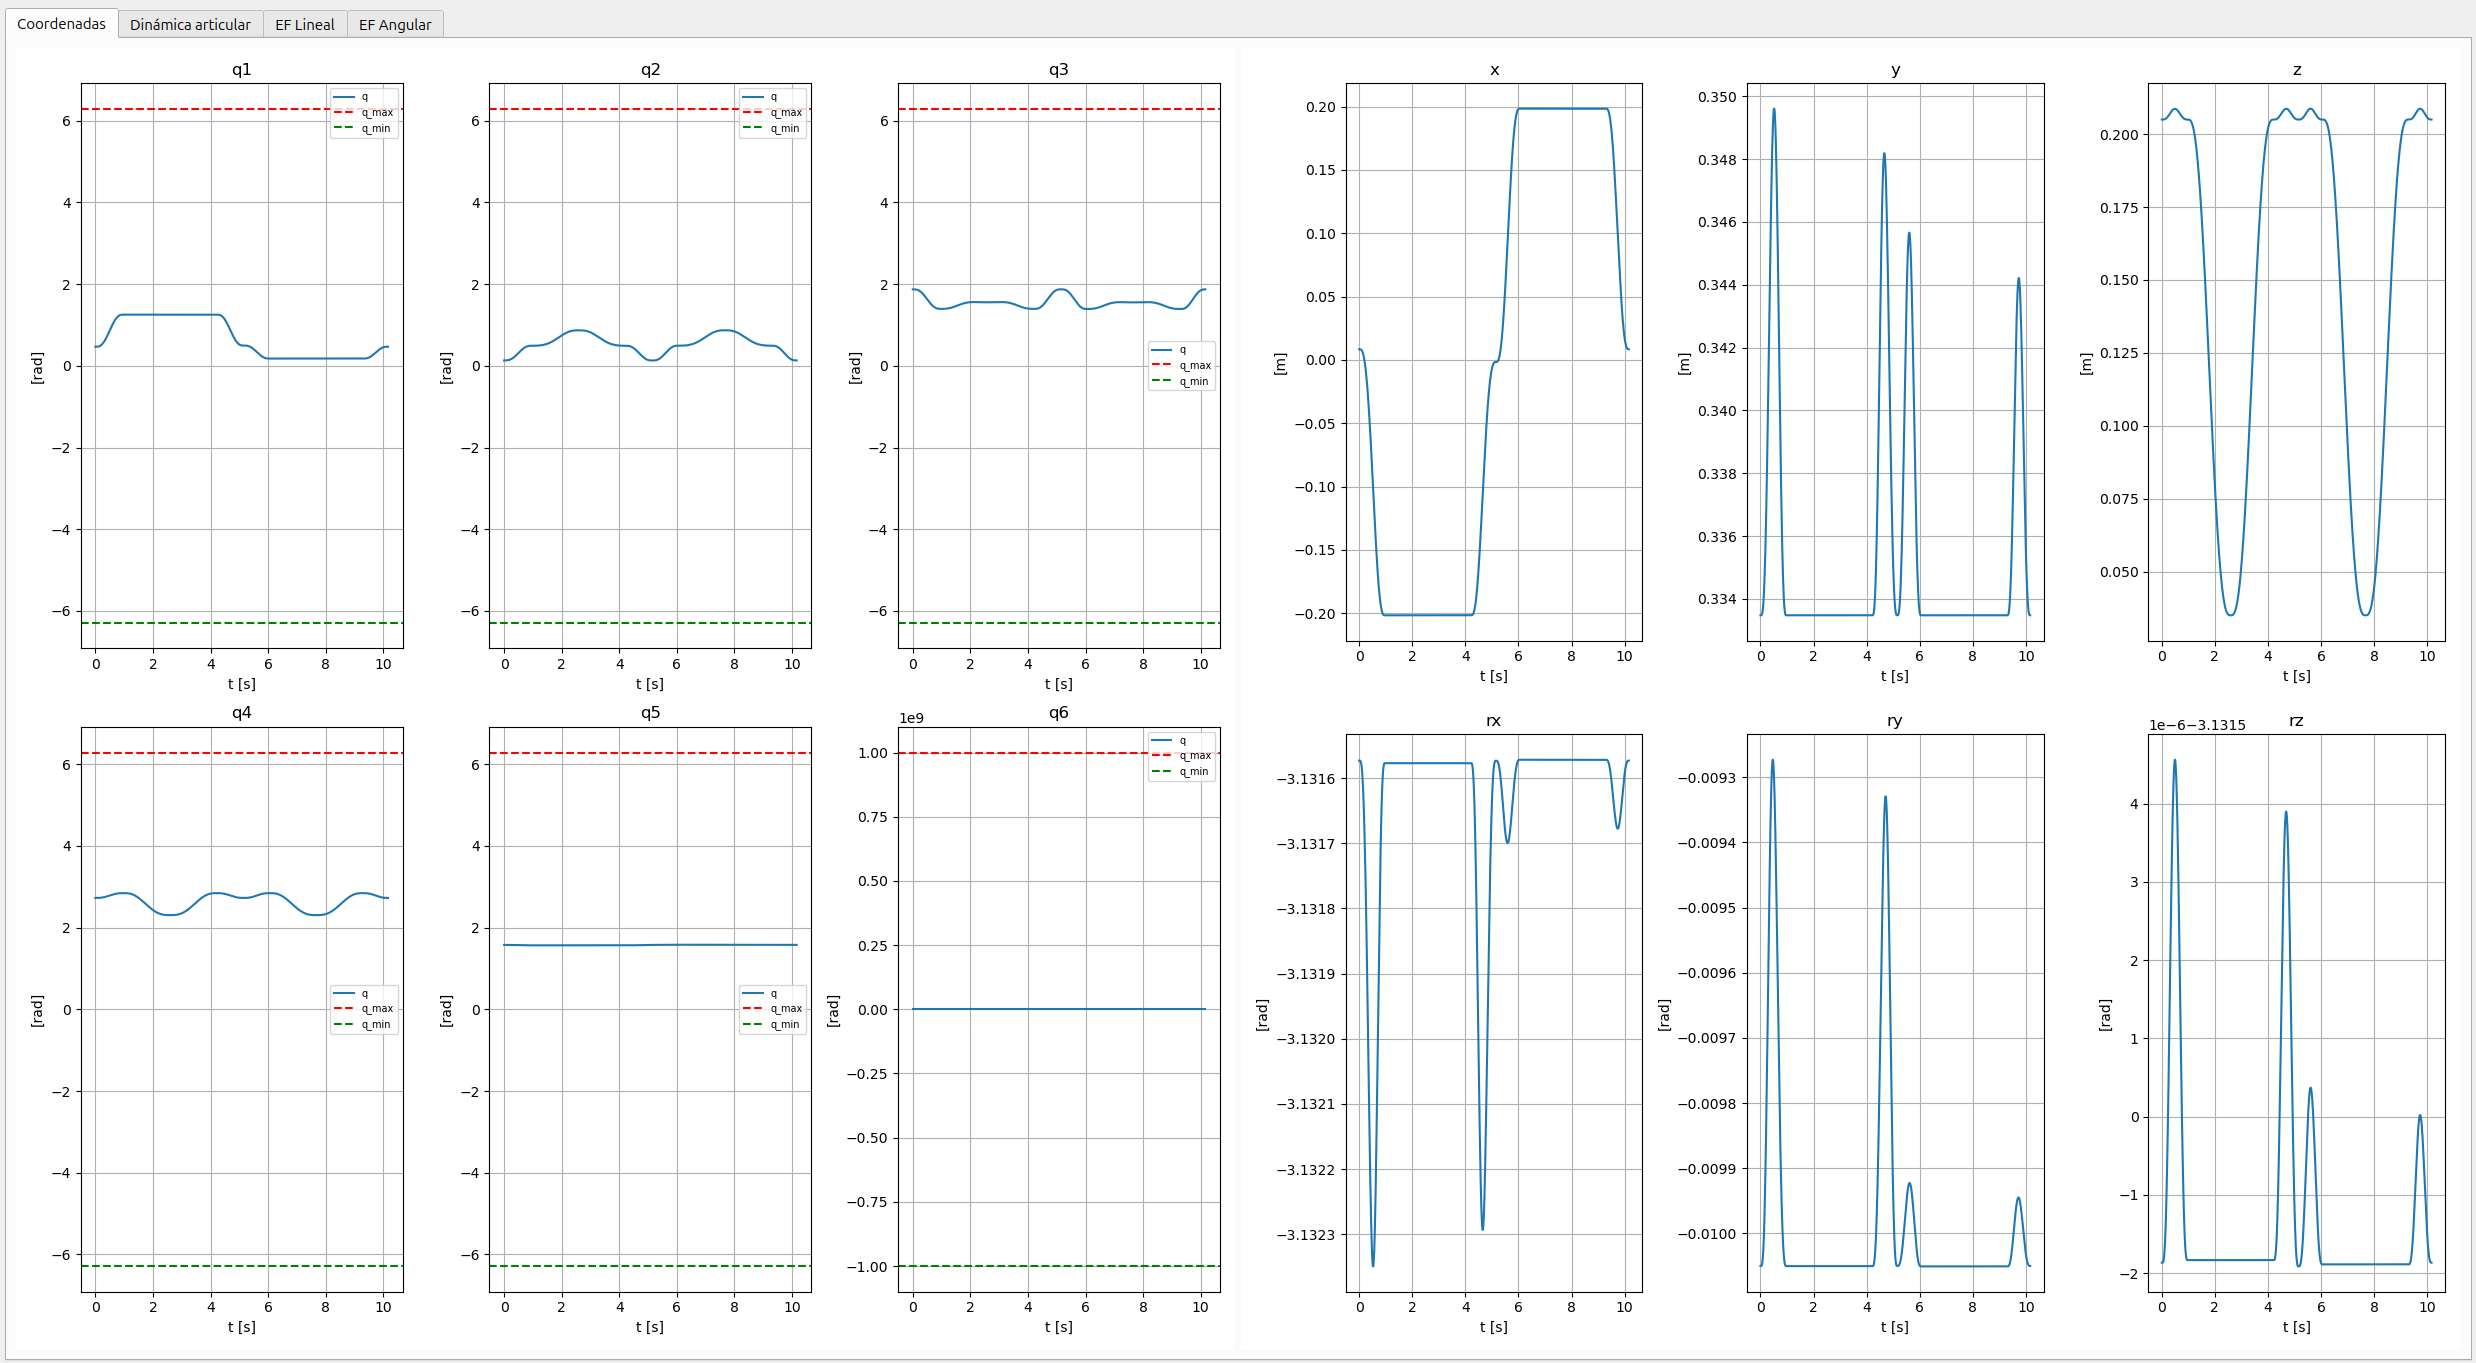
\includegraphics[width=\linewidth]{verif_an1.png}
    \caption{Evolución de posiciones articulares y coordenadas cartesianas del efector final durante el ciclo.}
    \label{fig:verif_an1}
\end{figure}

La figura~\ref{fig:verif_an2} presenta las velocidades y aceleraciones articulares junto con sus límites definidos.

\begin{figure}[H]
    \centering
    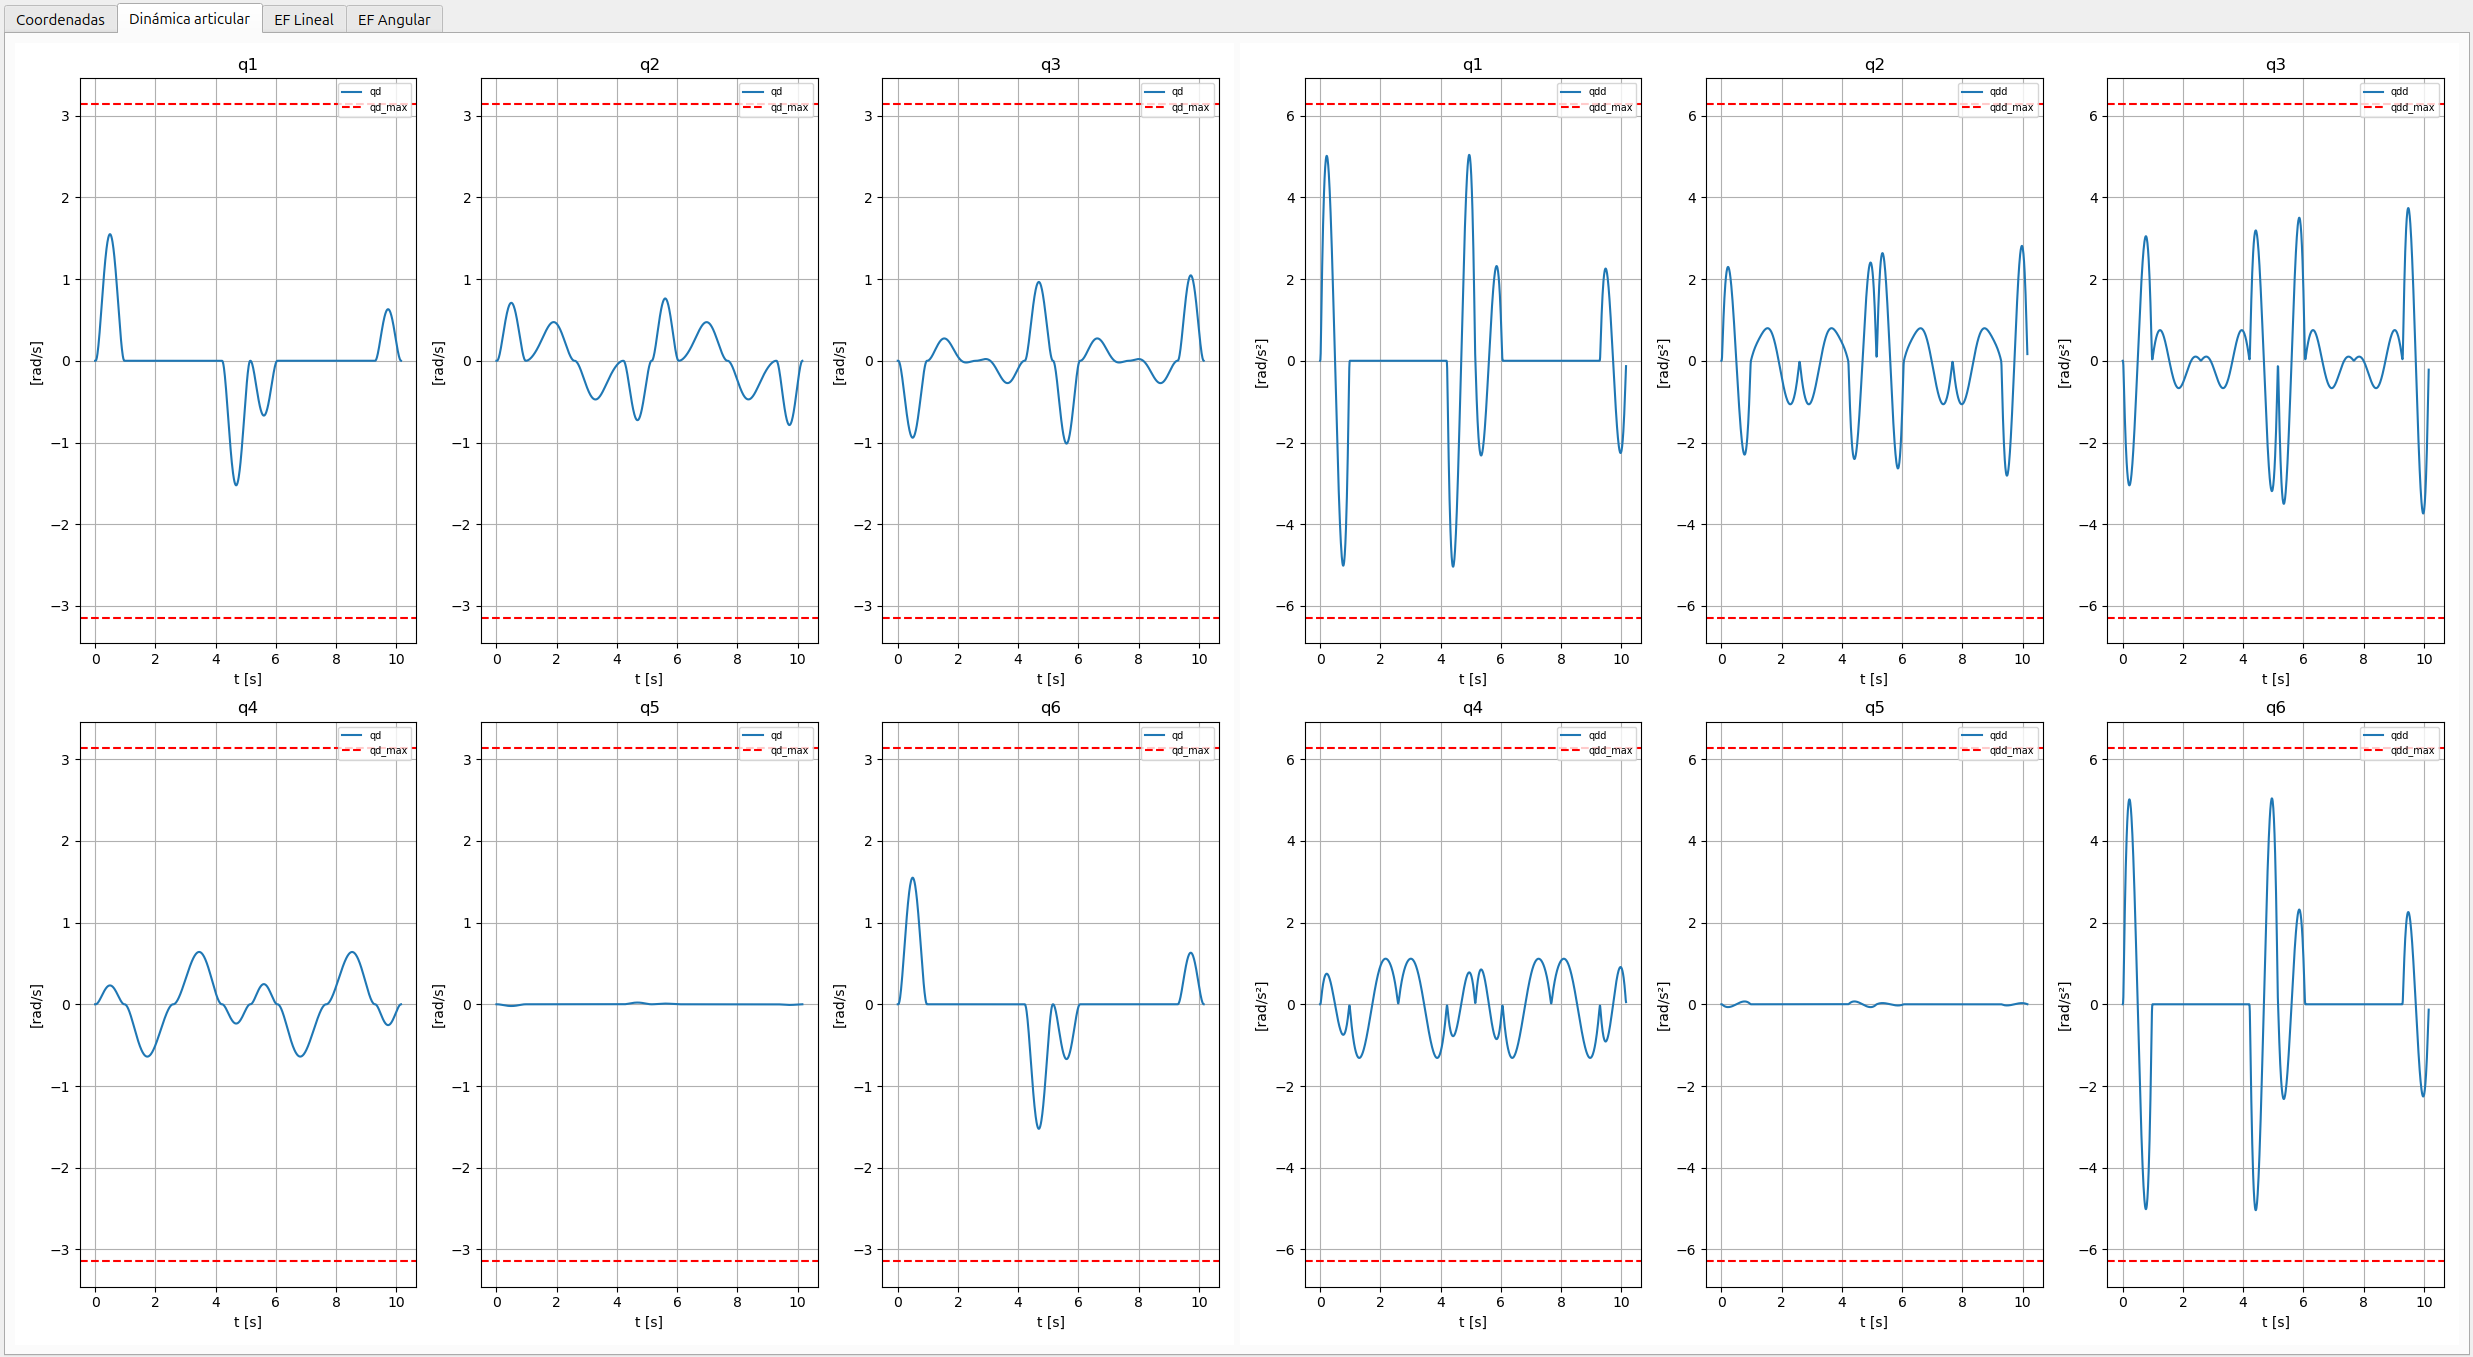
\includegraphics[width=\linewidth]{verif_an2.png}
    \caption{Evolución de velocidades y aceleraciones articulares durante el ciclo.}
    \label{fig:verif_an2}
\end{figure}

La figura~\ref{fig:verif_an3} muestra la velocidad y aceleración lineales del efector final calculadas a través del Jacobiano geométrico, en comparación con los límites establecidos.

\begin{figure}[H]
    \centering
    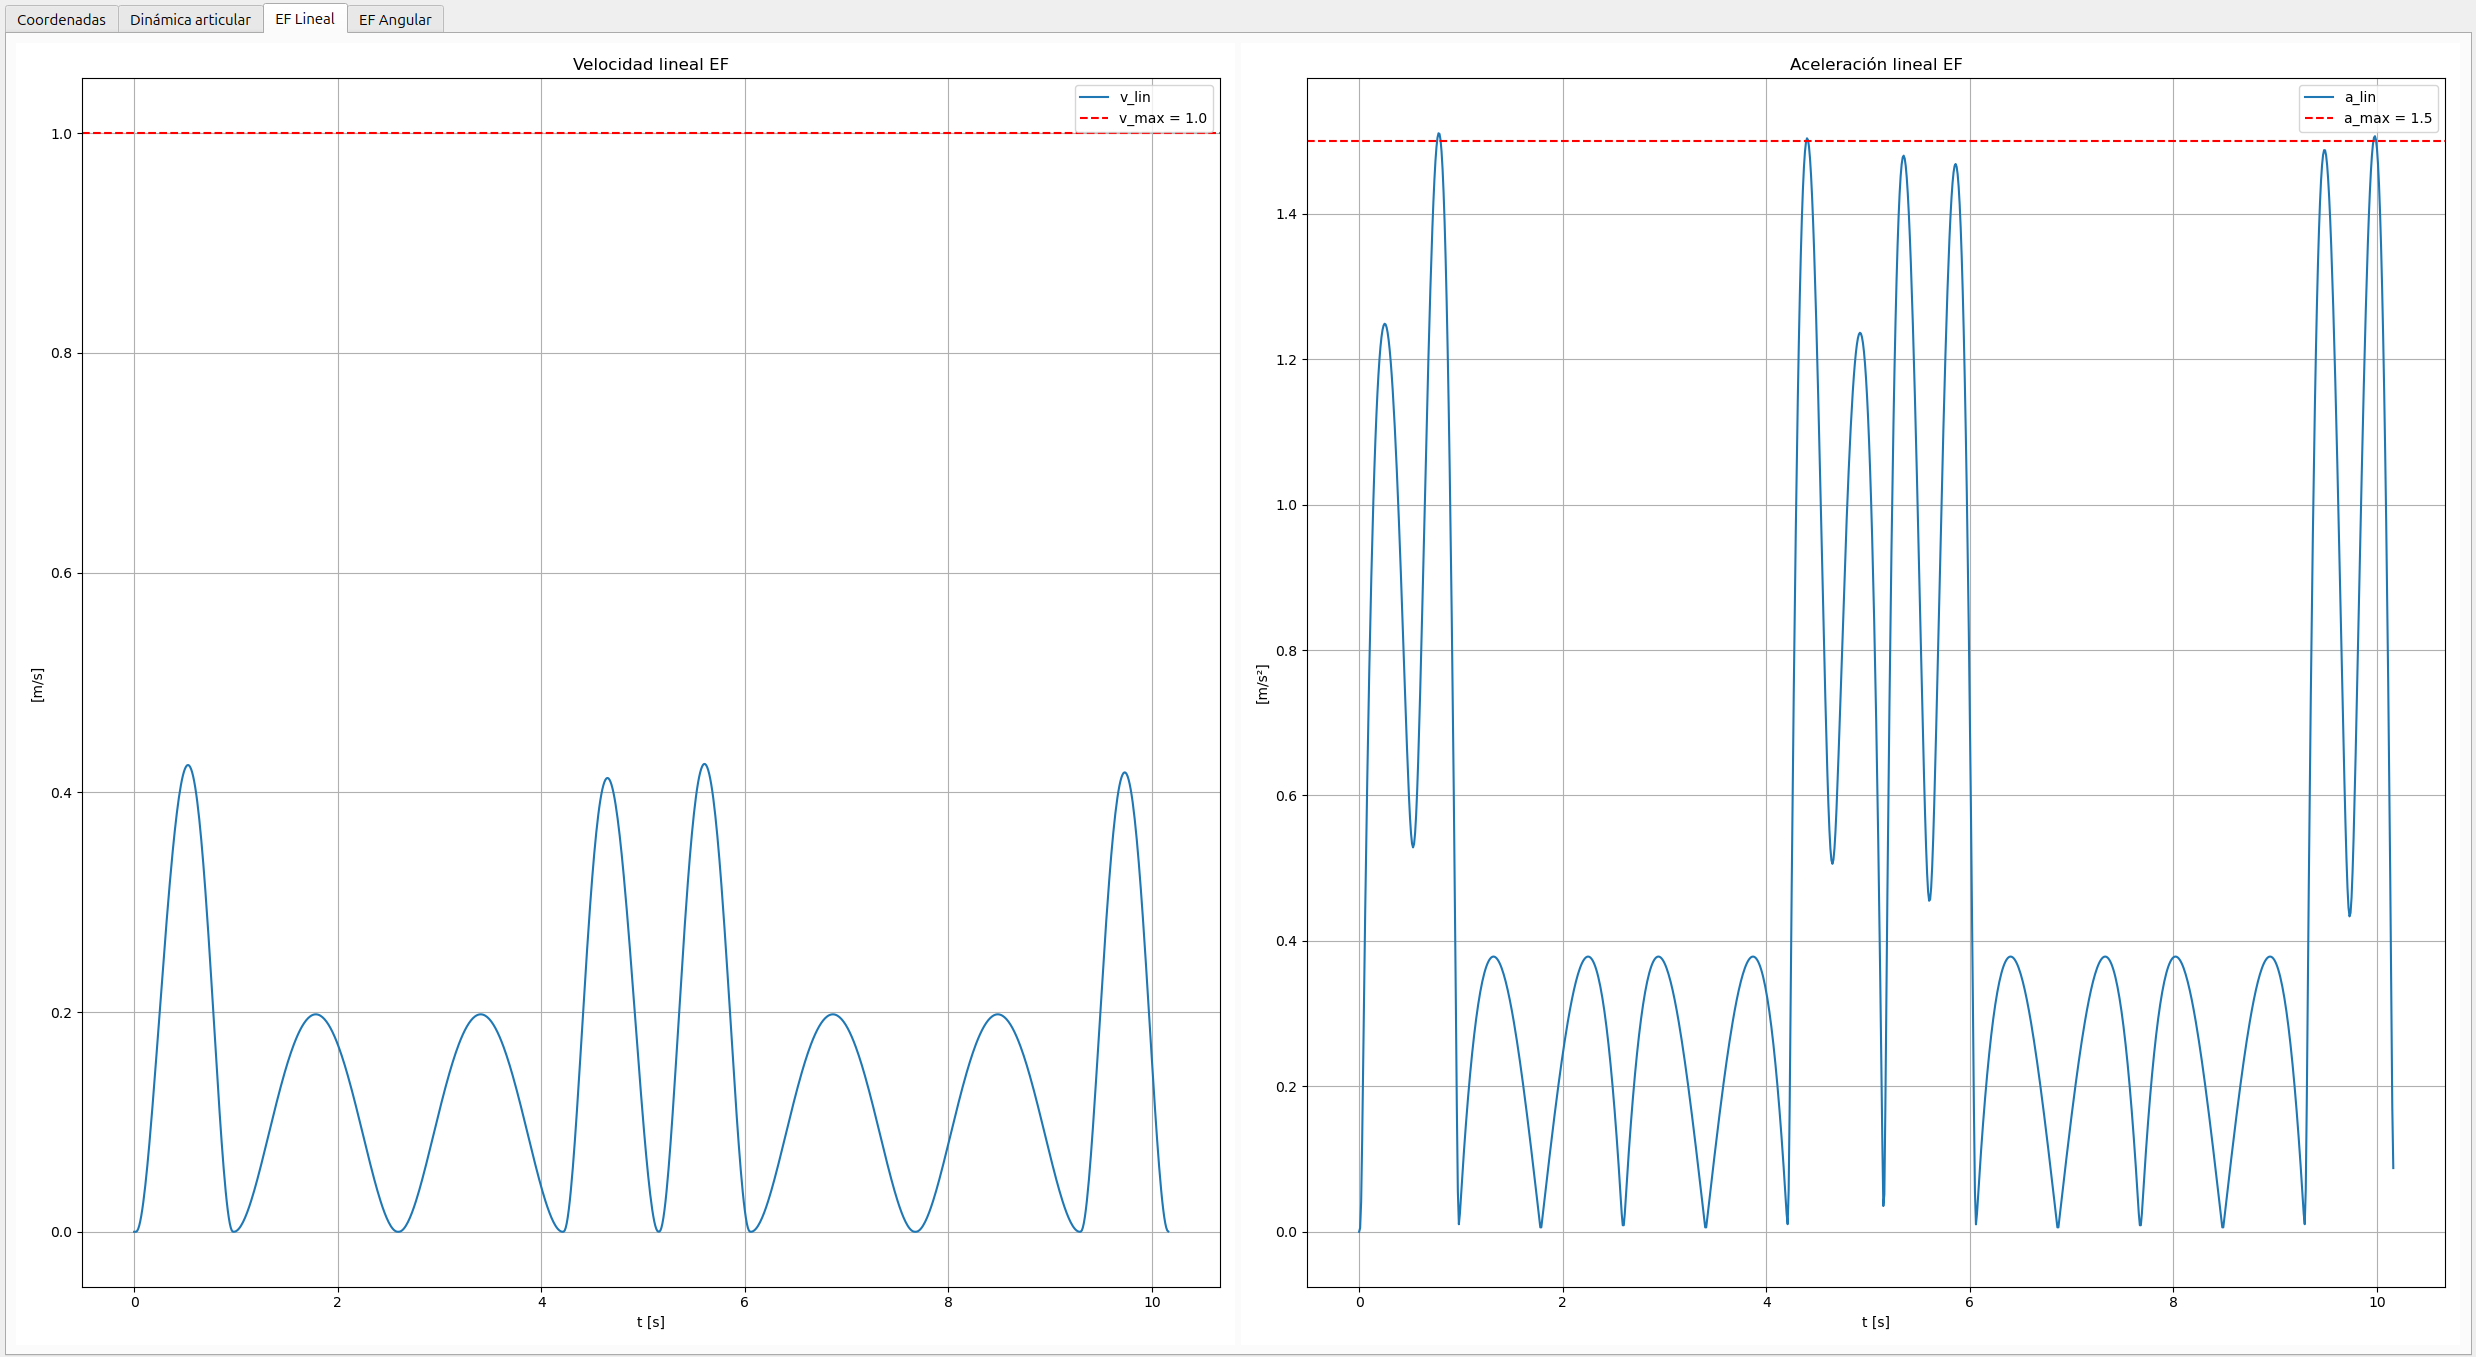
\includegraphics[width=\linewidth]{verif_an3.png}
    \caption{Evolución de velocidad y aceleración lineales del efector final durante el ciclo.}
    \label{fig:verif_an3}
\end{figure}

La figura~\ref{fig:verif_an4} presenta la velocidad y aceleración angulares del efector final con sus respectivos límites.

\begin{figure}[H]
    \centering
    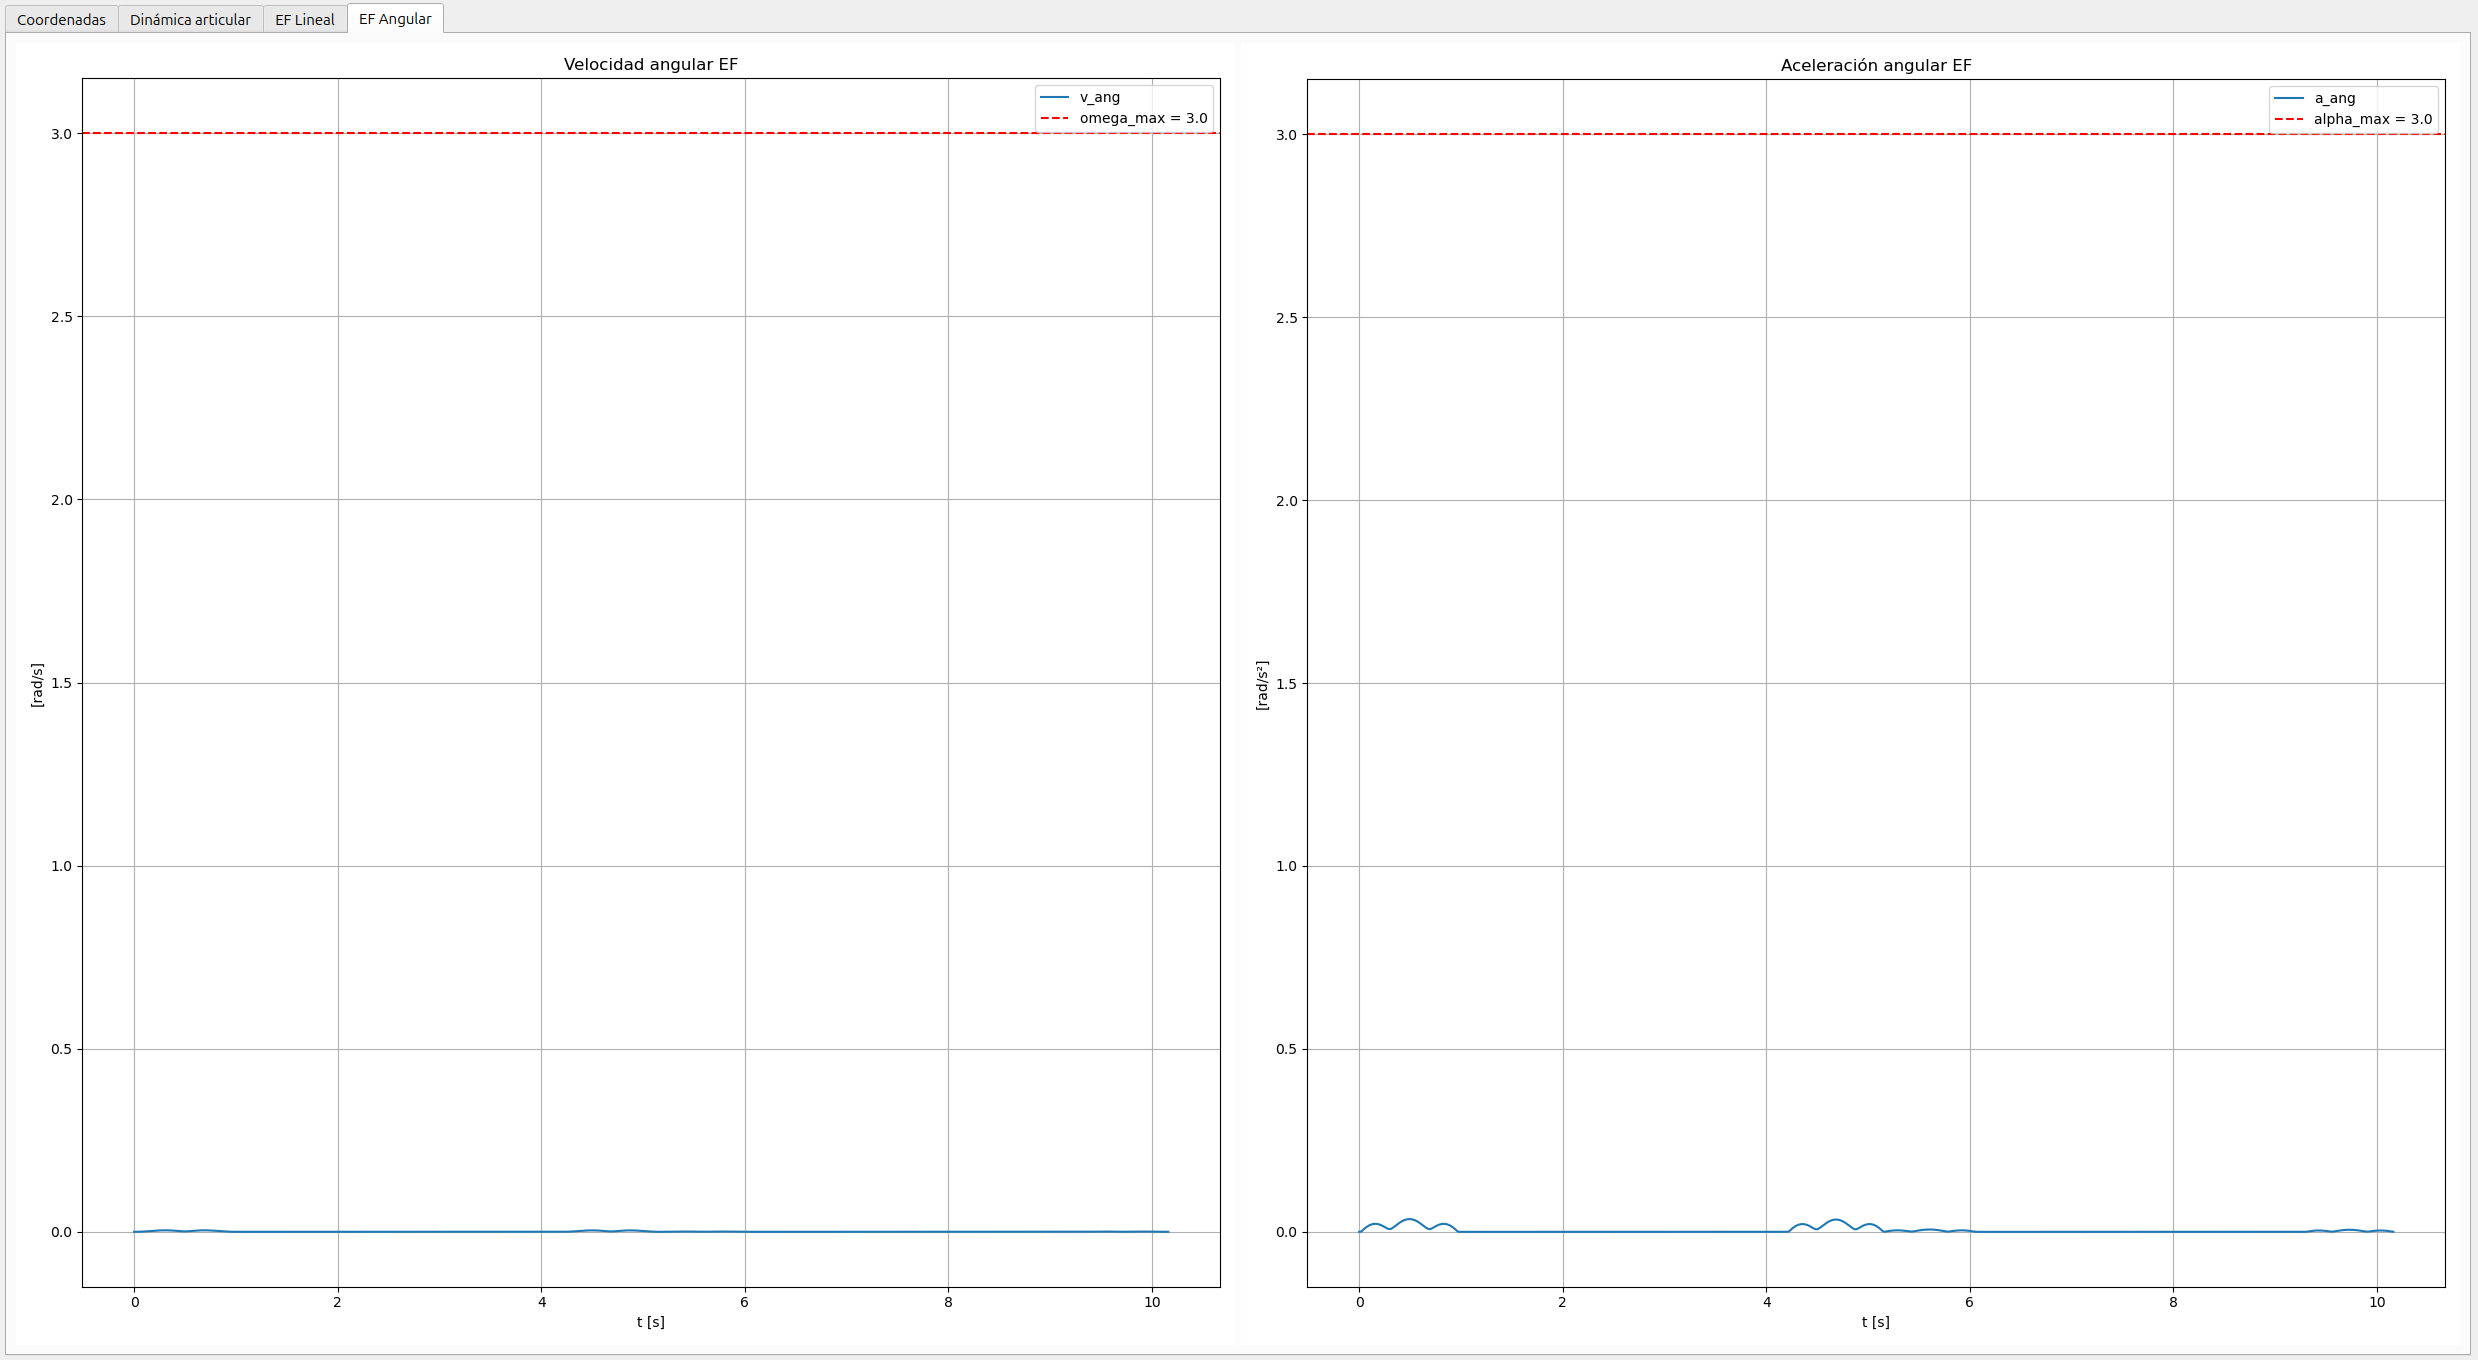
\includegraphics[width=\linewidth]{verif_an4.png}
    \caption{Evolución de velocidad y aceleración angulares del efector final durante el ciclo.}
    \label{fig:verif_an4}
\end{figure}

Del análisis se concluye que el ciclo operativo completo resulta en un tiempo de ejecución inferior a 10 segundos, lo que valida el cumplimiento del objetivo de productividad de 300 transferencias por hora. Asimismo, los perfiles de velocidad y aceleración tanto articulares como cartesianos se mantienen dentro de los límites cinemáticos definidos sin superarlos de forma considerable a lo largo de todo el ciclo.

% ======================================================================
\newpage
\section{Conclusiones y trabajo futuro}
\label{sec:conclusiones}

El presente trabajo logró cumplir con los objetivos planteados, desarrollando de forma íntegra el modelado cinemático, la simulación y la integración en software de robótica de un manipulador serial de seis grados de libertad orientado a tareas de automatización logística.

En la etapa de modelado, se aplicó la convención Denavit-Hartenberg para formular la cinemática directa del manipulador y se obtuvo una solución analítica cerrada de la cinemática inversa. Este enfoque, alternativo a los métodos numéricos iterativos, resultó eficaz para el robot estudiado y permitió obtener hasta 512 configuraciones articulares válidas para una misma pose del efector final, brindando una amplia base para la selección de la solución óptima en cada instante de la trayectoria. Se identificaron y caracterizaron analíticamente las tres singularidades geométricas del manipulador: de hombro, de codo y de muñeca.

El módulo de generación de trayectorias incorporó interpolación en espacio articular y cartesiano, con un mecanismo de escalado automático de velocidades y aceleraciones basado en el Jacobiano geométrico, garantizando en todo momento el respeto de los límites cinemáticos del sistema. La simulación de la tarea completa de \textit{bin-to-bin transfer} en MATLAB validó el correcto funcionamiento del conjunto, combinando segmentos de interpolación articular para los desplazamientos rápidos y segmentos de interpolación cartesiana para las maniobras de \textit{picking} y \textit{placing}.

El diseño CAD de los eslabones en \textit{Fusion 360} y su integración como mallas STL al entorno de simulación permitió verificar visualmente la coherencia geométrica entre el modelo cinemático y la representación tridimensional del robot.

Finalmente, la integración en ROS~2 trasladó toda la cadena cinemática a una arquitectura de nodos distribuida, desarrollada íntegramente desde cero y sin dependencias de librerías de robótica de alto nivel. Se implementaron interfaces de comunicación personalizadas, un modelo URDF derivado directamente de la parametrización DH, visualización en RViz2 y una interfaz gráfica de usuario en PyQt5 que centraliza el movimiento manual, la enseñanza de puntos, la gestión de trayectorias y el análisis de variables cinemáticas.

Se verificó la funcionalidad completa del sistema en este entorno y se validó el cumplimiento de los objetivos de productividad establecidos para la tarea. Como limitación identificada en esta etapa, el servicio de generación de trayectorias acepta un único punto por solicitud, lo que impide la interpolación continua entre puntos vía consecutivos y obliga al robot a detenerse en cada punto intermedio, a diferencia del comportamiento logrado en MATLAB.

\subsection*{Trabajo futuro}

A partir del estado actual del desarrollo, se identifican las siguientes líneas de extensión prioritarias:

\begin{enumerate}

    \item \textbf{Interpolación continua entre puntos vía en ROS~2.} Rediseñar el servicio \texttt{/dr/gen\_traj} para que acepte una lista completa de puntos vía en una única solicitud, replicando el comportamiento de \texttt{mstraj} en MATLAB. Esto eliminaría la detención del robot en cada punto intermedio y permitiría trayectorias continuas y fluidas en el entorno ROS~2.

    \item \textbf{Replanificación de trayectorias en tiempo real.} Incorporar un módulo de replanificación que, ante cambios en el entorno o desviaciones respecto a la trayectoria nominal, genere una trayectoria alternativa sin detener la ejecución. Una primera aproximación realista consiste en monitorear el determinante del Jacobiano durante la ejecución y disparar una replanificación automática al detectar proximidad a configuraciones singulares.

    \item \textbf{Detección y evasión de colisiones.} Integrar un módulo de verificación de colisiones que opere tanto sobre objetos del entorno como sobre la propia geometría del robot (\textit{self-collision}). Una implementación realista puede basarse en la representación simplificada del robot mediante esferas o cápsulas envolventes y en el uso de la biblioteca \textit{FCL} (\textit{Flexible Collision Library}), disponible en el ecosistema ROS~2.

    \item \textbf{Mejoras de simulación en ROS~2.} Extender la simulación para incorporar el comportamiento completo de la tarea: activación y desactivación del \textit{gripper} durante las maniobras de \textit{picking} y \textit{placing}, gestión del estado de la herramienta y visualización en RViz2 del objeto manipulado a lo largo de la trayectoria. Esto permitiría una validación más fiel del ciclo completo de trabajo del manipulador.

    \item \textbf{Robustez del sistema.} Mejorar el manejo de errores en los nodos de ROS~2 incorporando reintentos con \textit{timeout}, recuperación ante fallos de servicio y retroalimentación más detallada hacia la interfaz gráfica. Incorporar métricas de tiempo de ejecución por segmento de trayectoria para facilitar el ajuste fino de los perfiles de velocidad en función de los requerimientos de productividad.

\end{enumerate}

% ======================================================================
\newpage
\begin{appendices}
\section{Verificación y Validación de Módulos de Software de MATLAB y ROS~2}

%====
\subsection{Cinemática Inversa}
\label{ap:IK}

La verificación del correcto funcionamiento del módulo de cinemática inversa se realiza mediante el script \colorbox{gray!20}{\texttt{test\_inv\_kinematics.m}}. Este incluye 3 funcionalidades

\begin{enumerate}
    \item \textbf{Verificación redundante:} Se define una coordenada articular, se calcula la cinemática directa para obtener la coordenada cartesiana del efector final, sobre esta última se calcula la cinemática inversa con el módulo desarrollado. Se presentan los resultados dejando en evidencia la coordenada articular inicial y el conjunto obtenido mediante cinemática inversa, también se calcula la cinemática directa para cada solución obtenida permitiendo otro contraste de resultados. Finalmente, se realiza un resumen estadístico del error entre la coordenada cartesiana de entrada y las coordenadas cartesianas obtenidas a partir de cada solución articular, para verificar que el error se mantenga dentro de un rango aceptable.
\begin{lstlisting}[style=Matlab-editor, basicstyle=\small\ttfamily]
% ==INPUT ==
% Coordenadas articulares igresadas:
q = [1.8358    0.4922   -1.9151   -0.5557    1.7815    1.2078];
% Las coordenadas cartesianas consigna (calculadas mediante DK) son: 
x = -0.16918 | y = -0.19848 | z = 0.29694 | alpha = 2.7989 | beta = -0.3074 | gamma = 2.2087
% ==OUTPUT==
% Las coordenadas articulares solución obtenidas de la cinematica inversa son (solo algunas):
1.8358    0.4922   -1.9151   -0.5557    1.7815    1.2078
-4.4474    0.4922   -1.9151   -0.5557    1.7815    1.2078
-4.4474   -0.2860   -1.5354    2.9844    4.5017    4.3494
3.2637    0.2942   -4.8523   -3.1284    1.9973    2.7157
% Las coordenadas cartesianas solución obtenidas son las siguientes (se presentan solo algunas, todas coinciden):
x = -0.16918 | y = -0.19848 | z = 0.29694 | alpha = 2.7989 | beta = -0.3074 | gamma = 2.2087
x = -0.16918 | y = -0.19848 | z = 0.29694 | alpha = 2.7989 | beta = -0.3074 | gamma = 2.2087
x = -0.16918 | y = -0.19848 | z = 0.29694 | alpha = 2.7989 | beta = -0.3074 | gamma = 2.2087
x = -0.16918 | y = -0.19848 | z = 0.29694 | alpha = 2.7989 | beta = -0.3074 | gamma = 2.2087


% --- Resumen estadístico IK (poses aleatorias) ---
Poses testeadas:    300
Sin solución IK:    0
\end{lstlisting}
\begin{lstlisting}[basicstyle=\small\ttfamily]
  Poses verificadas:  300  (100.0%)
  Error posición    - max: 3.66e-06 m    prom: 2.06e-06 m
  Error orientación - max: 1.10e-05 rad  prom: 6.20e-06 rad
\end{lstlisting}

    \item \textbf{Cálculo directo: } Esta funcionalidad no se define específicamente para realizar una verificación sino para  conocer las coordenadas articulares solución de la cinemática inversa a partir de la coordenada cartesiana ingresada de forma directa. Los resultados se presentan de misma forma al ítem 1 dado que solo se realiza un \textit{override} durante ejecución de la coordenada cartesiana de entrada.
    \item \textbf{Verificación cíclica: } Esta funcionalidad permite, hasta que se detenga la ejecución del programa, verificar cíclicamente puntos aleatorios mediante un esquema de verificación similar al del ítem 1. De forma adicional, se calcula la norma entre coordenadas cartesianas de salida y de llegada, ante una diferencia mayor a un umbral determinado en cualquiera de las soluciones pertenecientes al conjunto de solución obtenido, se detiene el programa para verificar el error y poder analizarlo.
\begin{lstlisting}[style=Matlab-editor, basicstyle=\small\ttfamily]
% ==INPUT ==
% LOOP -> Probando posición articular
-3.2460   -1.2075   -5.0711   -4.6248    5.5550   -6.2832

% LOOP -> Las coordenadas cartesianas consigna son: 
x = 0.10246 | y = -0.40972 | z = 0.45372 | alpha = 3.0035 | beta = 0.83783 | gamma = 1.3635
% ==OUTPUT==
% Las coordenadas articulares solución obtenidas de la cinematica inversa son (solo algunas):
3.0372    0.7669   -1.7414   -0.5041    0.7282   -3.1416
-3.2460   -5.5163    4.5418    5.7791   -5.5550   -3.1416
-3.2460   -6.2786    5.0711   -3.4127   -0.7282         0
-2.2848    0.0199    0.9305   -3.2374    1.0729   -1.9493
% Resultado de norma:
OK
OK
OK
OK

\end{lstlisting}
\end{enumerate}

\textbf{NOTA:} En los resultados presentados, se mencionan solo una pequeña porción de toda la información devuelta por el script.

%====
\subsection{Singularidades}
\label{ap:SINGULARIDADES}

Para verificar que los patrones que conducen a singularidades determinados visualmente son correctos, se elabora el script \colorbox{gray!20}{\texttt{test\_singularities.m}}. En él se encuentra un ciclo \textit{while} infinito, solo terminable mediante finalización de ejecución. 

Para la singularidad de codo y de muñeca, se definen valores aleatorios para todas las variables articulares que no estén involucradas en el patrón de la singularidad, para las que sí están involucradas, se define un valor aleatorio dentro del conjunto de aquellos valores que puedan provocar la singularidad según las condiciones definidas en~\ref{sec:analisis_singularidades}.


Para la singularidad de hombro, debido a la presencia de 3 incógnitas en una misma ecuación, simplemente se busca verificar la observación, para esto, se dan valores aleatorios dentro de un rango de $\pm10º$ y con signo opuesto para $q_2$ y $q_3$, finalmente se busca el valor de $q_4$ que cumpla con la condición de proyección nula. El motivo por el que los valores para $q_2$ y $q_3$ están dentro del rango $\pm10º$ y de signo opuesto, es para evitar que la proyección no sea anulable geométricamente mediante $q_4$.


Para cada caso, se calcula el jacobiano en la configuración determinada y su determinante, solo en caso de que el determinante del jacobiano sea mayor al valor de umbral, de modo que no se considere cercano a una singularidad, se detiene la ejecución y se muestra información, caso contrario, la ejecución se repite cíclicamente informando cuando se completa cada ciclo. Un ciclo equivale al análisis de una configuración para el codo, una para la muñeca y una para el hombro.

A continuación se detalla un ejemplo para cada salida.

\begin{lstlisting}[style=Matlab-editor, basicstyle=\small\ttfamily]

    % == OUTPUT DE SINGULARIDAD VERIFICADA (TODAS CONFIGURACIONES SINGULARES) ==
    Ciclo completo - todas las posiciones fueron singulares - continuando...
    % == OUTPUT DE NO SINGULARIDAD ==
    Posición articular aleatoria - no singular - hombro
    1.7748   -0.1075    0.0635    0.4317   -0.3929    3.0684
    Determinante del Jacobiano: 7.897e-20
    -> Detención por posición no singular - enter para continuar

\end{lstlisting}

El último ejemplo, correspondiente a una salida negativa, se produjo exigiendo un determinante de jacobiano excesivamente pequeño para que la verificación falle intencionalmente. 
 
%====
\subsection{Generación de trayectorias}
\label{ap:generacion_trayectorias}

En la generación de trayectorias se buscan verificar dos aspectos fundamentales: que la trayectoria generada efectivamente interpole entre los puntos vía definidos y que el perfil de velocidades y aceleraciones resultante respete los límites cinemáticos establecidos. Para esto se elabora el script \colorbox{gray!20}{\texttt{test\_gen\_traj.m}} que contiene el siguiente procedimiento de verificación:
Se definen manualmente una serie de puntos vía con sus respectivos modos de interpolación (articular o cartesiano) y se genera la trayectoria utilizando el módulo desarrollado y se verifica:
\begin{enumerate}
    \item \textbf{Interpolación entre puntos vía:}  Se verifica que la trayectoria resultante efectivamente pase por cada uno de los puntos vía definidos, para esto, se calcula la distancia entre cada punto vía y el punto de la trayectoria correspondiente al mismo tiempo, verificando que esta distancia sea menor a un umbral determinado. En caso de detectar una cercanía lo suficientemente pequeña, se considera que el punto vía ha sido interpolado correctamente y se incrementa un contador.La verificación será positiva siempre que el contador sea mayor o igual al número total de puntos vía definidos.
    \item \textbf{Cumplimiento de límites cinemáticos:} Se imprime la comparativa entre valores máximos, perfiles cinemáticos iniciales y perfiles cinemáticos escalados para cumplir con límites. Se verifica: velocidad y aceleración angular de articulaciones, velocidad y aceleración líneal y angular de efector final. De este modo, la verificación será visual.
\end{enumerate}

Como complemento numérico a la verificación visual descripta, se presenta a continuación la salida del script \colorbox{gray!20}{\texttt{test\_gen\_traj.m}} para una trayectoria de prueba, donde se verifica el alcance los puntos vía y se contrastan los límites articulares y cinemáticos establecidos con los valores máximos efectivamente alcanzados a lo largo de la trayectoria escalada:

\begin{lstlisting}[basicstyle=\small\ttfamily]
N_alcanzados =

    60

Todos los puntos de control fueron alcanzados.
--- Verificación de límites articulares ---
  q1: límite = [-6.283, 6.283] rad | alcanzado = [-1.298, 1.391] rad
  q2: límite = [-6.283, 6.283] rad | alcanzado = [-0.403, 0.548] rad
  q3: límite = [-6.283, 6.283] rad | alcanzado = [-1.914, 1.021] rad
  q4: límite = [-6.283, 6.283] rad | alcanzado = [3.155, 3.508] rad
  q5: límite = [-6.283, 6.283] rad | alcanzado = [-1.584, 1.563] rad
  q6: límite = [-17453.293, 17453.293] rad | alcanzado = [-0.190, 0.785] rad

--- Verificación de velocidades y aceleraciones articulares ---
  qd1:  límite = 3.142 rad/s    | alcanzado = 0.530 rad/s
  qd2:  límite = 3.142 rad/s    | alcanzado = 0.151 rad/s
  qd3:  límite = 3.142 rad/s    | alcanzado = 0.758 rad/s
  qd4:  límite = 6.283 rad/s    | alcanzado = 0.089 rad/s
  qd5:  límite = 6.283 rad/s    | alcanzado = 0.792 rad/s
  qd6:  límite = 6.283 rad/s    | alcanzado = 0.261 rad/s
  qdd1: límite = 13.963 rad/s^2 | alcanzado = 1.208 rad/s^2
  qdd2: límite = 13.963 rad/s^2 | alcanzado = 0.343 rad/s^2
  qdd3: límite = 13.963 rad/s^2 | alcanzado = 1.728 rad/s^2
  qdd4: límite = 13.963 rad/s^2 | alcanzado = 0.203 rad/s^2
  qdd5: límite = 13.963 rad/s^2 | alcanzado = 1.807 rad/s^2
  qdd6: límite = 13.963 rad/s^2 | alcanzado = 0.596 rad/s^2

--- Verificación de velocidades y aceleraciones del efector final ---
  |v|:     límite = 1.000 m/s     | alcanzado = 0.330 m/s
  |a|:     límite = 1.500 m/s^2   | alcanzado = 0.739 m/s^2
  |w|:     límite = 3.000 rad/s   | alcanzado = 1.235 rad/s
  |alpha|: límite = 3.000 rad/s^2 | alcanzado = 3.098 rad/s^2
\end{lstlisting}

Se observa que la totalidad de los valores articulares y cartesianos alcanzados se mantiene dentro de los límites establecidos, con la única excepción de la aceleración angular del efector final, cuyo valor máximo (3.098~rad/s$^2$) supera marginalmente el límite definido (3.000~rad/s$^2$) en un instante puntual de la trayectoria, sin representar una superación considerable. A continuación puede observarse el impacto de los efectos de escalado en el perfil de velocidad en ambos dominios, articular y cartesiano:
\begin{figure}[H]
    \centering
    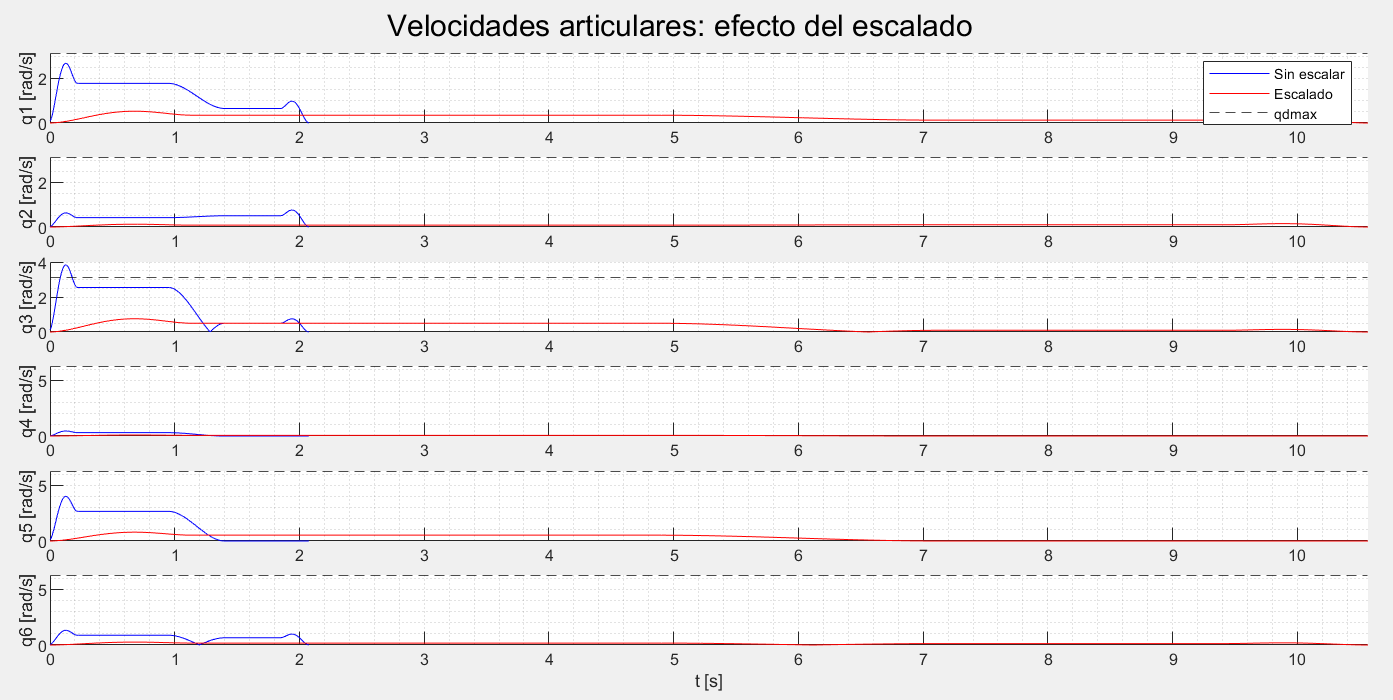
\includegraphics[width=0.85\linewidth]{verif_gen_traj_art.png}
    \caption{Comparativa entre perfiles de velocidad articular antes y después del escalado para cumplimiento de límites.}
    \label{fig:verif_gen_traj_vel}
\end{figure}

\begin{figure}[H]
    \centering
    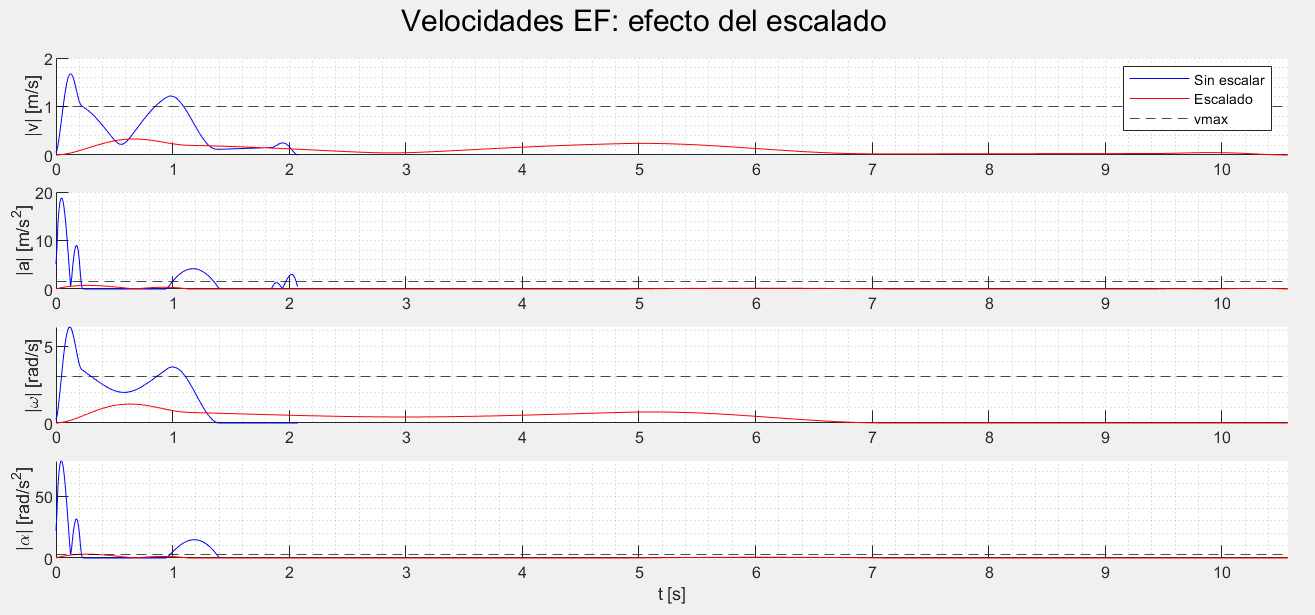
\includegraphics[width=0.85\linewidth]{verif_gen_traj_cart.png}
    \caption{Comparativa entre perfiles de velocidad cartesiana del efector final antes y después del escalado para cumplimiento de límites.}
    \label{fig:verif_gen_traj_vel_cart}
\end{figure}

%====
\subsection{Integración en ROS~2}
\label{ap:ros2_verificacion}

La verificación del sistema en ROS~2 se realizó de forma progresiva a lo largo del desarrollo, probando cada nodo de forma aislada antes de integrarlo con el resto del sistema. La metodología consistió en llamar directamente a los servicios y tópicos desde la terminal, sin depender de la interfaz gráfica, lo que permitió validar cada componente de forma independiente y detectar errores de comunicación, serialización y lógica en etapas tempranas.

A continuación se detallan los comandos más representativos utilizados durante este proceso:

\begin{itemize}

    \item \textbf{Inspección del grafo de nodos y tópicos activos:}
\begin{lstlisting}[language=bash, basicstyle=\footnotesize\ttfamily, breaklines=true, prebreak={}, postbreak={}]
ros2 node list
ros2 topic list
ros2 service list
\end{lstlisting}

    \item \textbf{Monitoreo del estado del robot en tiempo real} (pose articular y cartesiana publicada por el nodo de cinemática):
\begin{lstlisting}[language=bash, basicstyle=\footnotesize\ttfamily, breaklines=true, prebreak={}, postbreak={}]
ros2 topic echo /dr/robot_state
\end{lstlisting}

    \item \textbf{Llamada al servicio de cinemática directa} con una configuración articular manual:
\begin{lstlisting}[language=bash, basicstyle=\footnotesize\ttfamily, breaklines=true, prebreak={}, postbreak={}]
ros2 service call /dr/solve_fk dr_interfaces/srv/SolveFK "{q:[0.0,0.5,-1.0,0.0,1.5,0.0]}"
\end{lstlisting}

    \item \textbf{Llamada al servicio de cinemática inversa} a partir de una pose cartesiana objetivo:
\begin{lstlisting}[language=bash, basicstyle=\footnotesize\ttfamily, breaklines=true, prebreak={}, postbreak={}]
ros2 service call /dr/solve_ik dr_interfaces/srv/SolveIK "{pose:[-0.22,0.3,0.2,0.01,3.1416,0.01],q0:[0.0,0.0,0.0,0.0,1.5708,0.0],force:false}"
\end{lstlisting}

    \item \textbf{Generación de una trayectoria} desde la configuración actual hasta un punto cartesiano objetivo:
\begin{lstlisting}[language=bash, basicstyle=\footnotesize\ttfamily, breaklines=true, prebreak={}, postbreak={}]
ros2 service call /dr/gen_traj dr_interfaces/srv/GenTraj "{pose:[0.0,0.3,0.25,0.01,3.1416,0.01],mode:1,speed_profile:1}"
\end{lstlisting}

    \item \textbf{Guardado y listado de trayectorias} en el nodo de almacenamiento:
\begin{lstlisting}[language=bash, basicstyle=\footnotesize\ttfamily, breaklines=true, prebreak={}, postbreak={}]
ros2 service call /dr/list_trajs dr_interfaces/srv/ListTrajs "{}"
ros2 service call /dr/delete_traj dr_interfaces/srv/DeleteTraj "{name:'tarea_1'}"
\end{lstlisting}

    \item \textbf{Envío de un delta de teaching} para verificar el desplazamiento incremental del efector final:
\begin{lstlisting}[language=bash, basicstyle=\footnotesize\ttfamily, breaklines=true, prebreak={}, postbreak={}]
ros2 topic pub --once /dr/teaching_delta dr_interfaces/msg/TeachingDelta "{dx:0.01,dy:0.0,dz:0.0,droll:0.0,dpitch:0.0,dyaw:0.0}"
\end{lstlisting}

    \item \textbf{Ejecución de una trayectoria} mediante la acción \texttt{/dr/execute}: el goal recibe la trayectoria aplanada \texttt{q\_traj} y el entero \texttt{points}, por lo que desde consola se combina con la carga previa vía \texttt{/dr/load\_traj}. El feedback reporta el índice del punto en curso y el progreso porcentual:
\begin{lstlisting}[language=bash, basicstyle=\footnotesize\ttfamily, breaklines=true, prebreak={}, postbreak={}]
ros2 action send_goal /dr/execute dr_interfaces/action/Execute "{q_traj:[...],points:N}" --feedback
\end{lstlisting}

\end{itemize}

Este flujo de verificación incremental garantizó que cada nodo cumpliera su contrato de interfaz antes de ser integrado al sistema completo, reduciendo significativamente el tiempo de depuración en las etapas de integración.


% ======================================================================
\newpage
% BIBLIOGRAFÍA
\begin{thebibliography}{99}

  \bibitem{gvrGlobal2024}
    Grand View Research.\\
    \textit{Global Warehouse Robotics Market Size \& Outlook, 2023--2030}.\\
    2024.\\
    Disponible en: \url{https://www.grandviewresearch.com/horizon/outlook/warehouse-robotics-market-size/global}
    
  \bibitem{gvrUS2024}
    Grand View Research.  
    \textit{Warehouse Robotics Market Outlook: United States}.  
    2024.  
    Disponible en: \url{https://www.grandviewresearch.com/horizon/outlook/warehouse-robotics-market/united-states}


  \bibitem{gvrChina2024}
    Grand View Research.  
    \textit{Warehouse Robotics Market Outlook: China}.  
    2024.  
    Disponible en: \url{https://www.grandviewresearch.com/horizon/outlook/warehouse-robotics-market/china}


  \bibitem{gvrLatAm2024}
    Grand View Research.  
    \textit{Warehouse Robotics Market Outlook: Latin America}.  
    2024.  
    Disponible en: \url{https://www.grandviewresearch.com/horizon/outlook/warehouse-robotics-market/latin-america}


    
  \bibitem{gvrBrazil2024}
    Grand View Research.  
    \textit{Warehouse Robotics Market Outlook: Brazil}.  
    2024.  
    Disponible en: \url{https://www.grandviewresearch.com/horizon/outlook/warehouse-robotics-market/brazil}

    \bibitem{russellNorvig2021}
Stuart Russell \& Peter Norvig.  
\textit{Artificial Intelligence: A Modern Approach} (4th ed.).  
Pearson, 2021.  

\bibitem{craig2021}
John J. Craig.  
\textit{Introduction to Robotics: Mechanics and Control} (4th ed.).  
Pearson, 2021.  

\bibitem{corke2023}
Peter Corke.  
\textit{Robotics, Vision and Control: Fundamental Algorithms in MATLAB} (2nd ed.).  
Springer, 2023.  

\bibitem{ashby2022}
Michael F. Ashby.  
\textit{Materials Selection in Mechanical Design} (6th ed.).  
Elsevier, 2022.  

\bibitem{bathe2006}
Klaus-Jürgen Bathe.  
\textit{Finite Element Procedures}.  
Prentice Hall, 2006.  

\bibitem{krishnan2017}
Ramu Krishnan.  
\textit{Permanent Magnet Brushless DC Motor Drives and Controls}.  
CRC Press, 2017. 

\bibitem{martinez2024}
Aaron Martínez \& Enrique Fernández.  
\textit{Learning ROS 2: Basics, Concepts, and Practical Applications}.  
Packt, 2024.  

\bibitem{hyman2018}
Jesse H. Hyman.  
\textit{Learning Robotics Simulation Using ROS and Gazebo}.  
Packt, 2018.
\end{thebibliography}

\end{appendices}

\end{document}
